\documentclass[letterpaper,10pt]{memoir}
  \usepackage[latin1]{inputenc}
  \usepackage[T1]{fontenc}
  \usepackage[english,francais]{babel}
  \usepackage{vgmath,actu,amsmath,amsthm,icomma,url,natbib}
  \usepackage{palatino,mathpazo}
  \usepackage{textcomp,fourier-orns,mathabx}
  \usepackage{Sweave-sans-ae}
  \usepackage{threeparttable,paralist,expdlist}
  \usepackage{listings,answers}

  %%% Page titre
  \title{\HUGE Introduction � la programmation en S}
  \author{\huge Vincent Goulet \\[3mm]
    \large \textit{�cole d'actuariat, Universit� Laval}}
  \date{\Large Version 1.0}
  \newcommand{\ISBN}{2-9809136-0-X}

  %%% Commandes pour notes marginales
  \newcommand{\R}{\marginpar[\hfill \sffamily R]{\sffamily R}}
  \newcommand{\Splus}{\marginpar[\hfill S$+$]{S$+$}}
  \newcommand{\warning}{\marginpar[\hfill\LARGE\danger]%
    {\LARGE\danger}}
  \setlength{\marginparsep}{7mm}
  \setlength{\marginparwidth}{13mm}

  %%% Style des ent�tes de chapitres
  \chapterstyle{hangnum}

  %%% Styles des ent�tes et pieds de page
  \setlength{\headwidth}{\textwidth}
  \addtolength{\headwidth}{\marginparsep}
  \addtolength{\headwidth}{\marginparwidth}

  %%% Num�roter les sous-sections
  \maxsecnumdepth{subsection}
  \setsecnumdepth{subsection}

  %%% Styles pour les environnements d'exemples et al.
  \theoremstyle{plain}
  \newtheorem{ex}{Exemple}[chapter]
  \theoremstyle{remark}
  \newtheorem*{rem}{Remarque}
  \theoremstyle{definition}
  \newtheorem*{astuce}{Astuce}
  \newenvironment{sol}{\begin{proof}[Solution]}{\end{proof}}

  %%% Environnements pour les exercices et r�ponses. On utilise
  %%% \thechapter plut�t que \arabic{chapter} pour la num�rotation des
  %%% exercices dans les annexes.
  \Newassociation{rep}{reponse}{reponses}
  \newcounter{exercice}[chapter]
  \newenvironment{exercice}{%
    \begin{list}{\bfseries \thechapter.\arabic{exercice}}{%
        \refstepcounter{exercice}
        \settowidth{\labelwidth}{\bfseries \thechapter.\arabic{exercice}}
        \setlength{\leftmargin}{\labelwidth}
        \addtolength{\leftmargin}{\labelsep}
        \setdefaultenum{(a)}{(i)}{}{}}\item}
    {\end{list}}
  \renewenvironment{reponse}[1]{%
    \begin{list}{\bfseries #1}{%
        \settowidth{\labelwidth}{#1}
        \setlength{\leftmargin}{\labelwidth}
        \addtolength{\leftmargin}{\labelsep}
        \setdefaultenum{(a)}{(i)}{}{}}\item}
    {\end{list}}
  \renewcommand{\reponseparams}{{\thechapter.\theexercice}}

  %%% Environnement pour les listes de commandes
  \newenvironment{ttscript}[1]{%
    \begin{list}{}{%
        \setlength{\labelsep}{1.5ex}
        \settowidth{\labelwidth}{\code{#1}}
        \setlength{\leftmargin}{\labelwidth}
        \addtolength{\leftmargin}{\labelsep}
        \setlength{\parsep}{0.5ex plus0.2ex minus0.2ex}
        \setlength{\itemsep}{0.3ex}
        \renewcommand{\makelabel}[1]{##1\hfill}}}
    {\end{list}}

  %%% Environnement pour les listes de structures de contr�le
  \newenvironment{struclist}{%
    \begin{description}[\breaklabel\setlabelstyle{\mdseries\ttfamily}%
      \setleftmargin{\parindent}]}
    {\end{description}}

  %%% Param�tres pour les sections de code source
  \lstloadlanguages{R}
  \lstdefinelanguage{Renhanced}[]{R}{%
    morekeywords={acf,ar,arima,arima.sim,colMeans,colSums,is.na,is.null,%
      mapply,ms,na.rm,nlmin,replicate,row.names,rowMeans,rowSums,seasonal,%
      sys.time,system.time,ts.plot,which.max,which.min},
    deletekeywords={c},
    alsoletter={.\%},%
    alsoother={:_\$}}
  \lstset{language=Renhanced,extendedchars=true,
    basicstyle=\small\ttfamily,
    commentstyle=\textsl,
    keywordstyle=\mdseries,
    showstringspaces=false,
    index=[1][keywords], 
    indexstyle=\indexfonction}

  %%% Styles pour les noms de fonctions, code, etc.
  \newcommand{\code}[1]{\texttt{#1}}

  %%% Index
  \renewcommand{\preindexhook}{%
    Les num�ros de page en caract�res gras indiquent les pages o� les
    concepts sont introduits, d�finis ou expliqu�s.\vskip\onelineskip}
  \newcommand{\Index}[1]{\index{#1|textbf}}
  \newcommand{\indexargument}[1]{\index{#1@\code{#1}}}
  \newcommand{\Indexargument}[1]{\Index{#1@\code{#1}}}
  \newcommand{\indexattribut}[1]{\index{#1@\code{#1} (attribut)}}
  \newcommand{\Indexattribut}[1]{\Index{#1@\code{#1} (attribut)}}
  \newcommand{\indexclasse}[1]{\index{#1@\code{#1} (classe)}}
  \newcommand{\Indexclasse}[1]{\Index{#1@\code{#1} (classe)}}
  \newcommand{\indexfonction}[1]{\index{#1@\code{#1}}}
  \newcommand{\Indexfonction}[1]{\Index{#1@\code{#1}}}
  \newcommand{\indexmode}[1]{\index{#1@\code{#1} (mode)}}
  \newcommand{\Indexmode}[1]{\Index{#1@\code{#1} (mode)}}
  \newcommand{\indexobjet}[1]{\index{#1@\code{#1}}}
  \newcommand{\Indexobjet}[1]{\Index{#1@\code{#1}}} 
  \newcommand{\indexemacs}[1]{\index{Emacs!#1@\texttt{#1}}}
  \newcommand{\indexess}[1]{\index{ESS!#1@\texttt{#1}}}

  \newcommand{\attribut}[1]{\code{#1}\indexattribut{#1}}
  \newcommand{\Attribut}[1]{\code{#1}\Indexattribut{#1}}
  \newcommand{\argument}[1]{\code{#1}\indexargument{#1}}
  \newcommand{\Argument}[1]{\code{#1}\Indexargument{#1}}
  \newcommand{\classe}[1]{\code{#1}\indexclasse{#1}}
  \newcommand{\Classe}[1]{\code{#1}\Indexclasse{#1}}
  \newcommand{\fonction}[1]{\code{#1}\indexfonction{#1}}
  \newcommand{\Fonction}[1]{\code{#1}\Indexfonction{#1}}
  \newcommand{\mode}[1]{\code{#1}\indexmode{#1}}
  \newcommand{\Mode}[1]{\code{#1}\Indexmode{#1}}
  \newcommand{\objet}[1]{\code{#1}\indexobjet{#1}}
  \newcommand{\Objet}[1]{\code{#1}\Indexobjet{#1}}
  \newcommand{\emacs}[1]{\code{#1}\indexemacs{#1}}
  \newcommand{\ess}[1]{\code{#1}\indexess{#1}}
  \makeindex

%  \includeonly{presentation}

\begin{document}

\renewcommand{\FrenchLabelItem}{\small$\sqbullet$}
\renewcommand{\labelitemii}{\textendash}

\shortcites{Rintro}

\frontmatter

\pagestyle{empty}
\newlength{\gauche}
\newlength{\droite}

\calccentering{\unitlength}
\addtolength{\gauche}{\unitlength}
\addtolength{\gauche}{-1.5cm}
\addtolength{\droite}{\unitlength}
\addtolength{\droite}{1.5cm}
\begin{adjustwidth*}{\gauche}{-\droite}
  \centering
  \vspace*{2cm}
  \thetitle \\
\end{adjustwidth*}
\cleardoublepage

\begin{adjustwidth*}{\gauche}{-\droite}
  \centering
  \vspace*{2cm}
  \thetitle \\
  \vspace*{3cm}
  \theauthor \\
  \vspace*{\fill}
  \thedate
\end{adjustwidth*}
\clearpage

\begingroup
\begin{adjustwidth*}{\unitlength}{-\unitlength}
  \footnotesize 
  \setlength{\parindent}{0pt}
  \setlength{\parskip}{\baselineskip}
  
  \textcopyright{} 2005 Vincent Goulet \\
  Tous droits r�serv�s

  Il est permis de copier, distribuer et/ou modifier ce document selon
  les termes de la GNU Free Documentation License, Version 1.2 ou
  toute version subs�quente publi�e par la Free Software Foundation;
  avec aucune section inalt�rable (\emph{Invariant Sections}), aucun
  texte de couverture avant (\emph{Front-Cover Texts}), et aucun texte
  de couverture arri�re (\emph{Back-Cover Texts}). Une copie de la
  licence est incluse dans l'annexe \ref{fdl}.

  \begin{center}
    \begin{tabular}{ll}
      Version 0.99: & 29 novembre 2005 \\
      Version 0.9:  & 9 novembre 2005 \\
      Version 0.8:  & 16 septembre 2005 \\
    \end{tabular}
  \end{center}

  \textbf{Avis de marque de commerce} \\
  S-Plus\textregistered{} est une marque d�pos�e de Insightful
  Corporation.
\end{adjustwidth*}
\endgroup
\clearpage

%%% Local Variables: 
%%% mode: latex
%%% TeX-master: "introduction_programmation_S"
%%% End: 


\pagestyle{companion}
\chapter*{Pr�face}
\addcontentsline{toc}{chapter}{Pr�face}
\markboth{Pr�face}{Pr�face}


Il existe d�j� de multiples ouvrages traitant de S-Plus ou \textsf{R}.
Dans la majorit� des cas, toutefois, ces deux logiciels sont pr�sent�s
dans le cadre d'applications statistiques sp�cifiques. Cet ouvrage se
concentre plut�t sur l'apprentissage du langage de programmation
sous-jacent aux diverses fonctions statistiques, le S.

Ce texte est la somme de notes et d'exercices de diff�rents cours
donn�s par l'auteur � l'�cole d'actuariat de l'Universit� Laval depuis
septembre 2003. Les six premiers chapitres, qui constituent le
c{\oe}ur du document, proviennent d'une partie d'un cours o� l'accent
est mis sur l'apprentissage d'un (deuxi�me) langage de programmation
par des �tudiants de premier cycle en sciences actuarielles. Les
applications num�riques et statistiques de S-Plus et \textsf{R}
viennent plus tard dans le cursus universitaire et c'est alors que les
concepts des chapitres \ref{optimisation}, \ref{regression} et
\ref{ts} sont �tudi�s.

Les cours d'introduction au langage S sont donn�s � raison d'une heure
par semaine de cours magistral suivie de deux heures en laboratoire
d'informatique. C'est ce qui explique la structure des six premiers
chapitres: les �l�ments de th�orie, contenant peu voire aucun exemple,
sont pr�sent�s en rafale en classe. Puis, lors des s�ances de
laboratoire, les �tudiantes et �tudiants sont appel�s � lire et
ex�cuter les exemples se trouvant � la fin des chapitres. Chaque
section d'exemples couvre l'essentiel des concepts pr�sent�s dans le
chapitre et les compl�mente souvent. L'�tude de ces sections fait donc
partie int�grante de l'apprentissage du langage S.

Le texte des sections d'exemples est disponible en format �lectronique
dans le site Internet
\begin{quote}
  \url{http://vgoulet.act.ulaval.ca/pub/intro_S}
\end{quote}

Certains exemples et exercices trahissent le premier public de ce
document: on y fait � l'occasion r�f�rence � des concepts de base de
la th�orie des probabilit�s et des math�matiques financi�res. Les
contextes actuariels demeurent n�anmoins peu nombreux et ne devraient
g�n�ralement pas d�router le lecteur moins familier avec ces notions.

Les chapitres \ref{optimisation} (fonctions d'optimisation),
\ref{regression} (r�gression lin�aire) et \ref{ts} (s�ries
chronologiques) sont structur�s de mani�re plus classique, notamment
parce que le texte y est en prose. Ces chapitres comportent n�anmoins
des sections d'exemples.

Le texte prend partie en faveur de l'utilisation de GNU Emacs et du
mode ESS pour l'�dition de code S.  Les annexes contiennent de
l'information sur l'utilisation de S-Plus et \textsf{R} avec cet
�diteur. On y traite �galement des g�n�rateurs de nombres al�atoires
et de la planification d'une �tude de simulation en S.

Dans la mesure du possible, cet ouvrage t�che de pr�senter les
environnements S-Plus et \textsf{R} en parall�le et en soulignant
leurs diff�rences, lorsqu'elles surviennent. Les informations propres
� S-Plus ou \textsf{R} sont d'ailleurs identifi�es en marge par les
marques �S$+$� et �\textsf{R}�, respectivement.  �tant donn� la nette
pr�f�rence de l'auteur pour \textsf{R}, les divers extraits de code
ont g�n�ralement �t� ex�cut�s avec ce moteur S.

� moins d'erreurs et d'omissions (que les lecteurs sont invit�s � nous
faire conna�tre), les informations donn�es � propos de S-Plus sont
exactes pour les versions 6.1 (Linux et Windows), 6.2 Student Edition
(Windows) et 7.0 (Linux et Windows). Pour \textsf{R}, la version 2.2.0
(Linux et Windows), soit la plus r�cente lors de la r�daction, a �t�
utilis�e comme r�f�rence.

On notera enfin que cet ouvrage n'a aucune pr�tention d'exhaustivit�.
C'est d'ailleurs pourquoi on r�f�re fr�quemment au livre de
\cite{MASS}, plus complet.

L'auteur tient � remercier M.~Mathieu Boudreault pour sa collaboration
dans la r�daction des exercices.

\begin{flushright}
  \itshape
  Vincent Goulet \url{<vincent.goulet@act.ulaval.ca>} \\
  Qu�bec, novembre 2005
\end{flushright}


%%% Local Variables: 
%%% mode: latex
%%% TeX-master: "introduction_programmation_S"
%%% End: 

\tableofcontents*

\mainmatter
\section{Pr�sentation du langage S}


\subsection{Le langage S}

\begin{frame}
  \frametitle{Un langage pour �programmer avec des donn�es�}

  \begin{itemize}
  \item D�velopp� chez Bell Laboratories
  \item Langage de programmation complet et autonome
  \item Inspir� de plusieurs langages, dont l'APL et le Lisp:
    \begin{itemize}
    \item interpr�t� (et non compil�)
    \item sans d�claration obligatoire des variables
    \item bas� sur la notion de vecteur
    \item particuli�rement puissant pour les applications
      math�matiques et statistiques (et donc actuarielles)
    \end{itemize}
  \end{itemize}
\end{frame}


\subsection{Les moteurs S}

\begin{frame}
  \frametitle{Deux �moteurs� ou dialectes du langage S}

  \begin{itemize}
  \item Jusqu'� r�cemment, le plus connu �tait S-PLUS de Insightful
    Corporation, maintenant S$+$ de Timbco Software
  \item Le leader est maintenant \textsf{R}, ou GNU S, est une version
    libre (\emph{Open Source}) �\emph{not unlike S}�
  \item Environnements int�gr�s de manipulation de donn�es, de calcul
    et de pr�paration de graphiques
  \end{itemize}
\end{frame}


\subsection[Interfaces]{Interfaces pour S-Plus et R}

\begin{frame}
  \frametitle{D'abord des applications en ligne de commande}

  \begin{itemize}
  \item S$+$ poss�de une interface graphique �labor�e qui permet
    d'utiliser le logiciel sans trop conna�tre le langage de
    programmation
  \item \textsf{R} dispose �galement d'une interface graphique sous
    Windows et Mac OS
  \item L'�dition s�rieuse de code S b�n�ficie cependant grandement
    d'un bon �diteur de texte
  \end{itemize}
\end{frame}

\begin{frame}
  \begin{itemize}
  \item Question 6.2 de la foire aux questions (FAQ) de
    \textsf{R}: �Devrais-je utiliser \textsf{R} � l'int�rieur de
    Emacs?�
  \item R�ponse: �Oui, tout � fait�
  \item Nous apprendrons � utiliser \textsf{R} � l'int�rieur de GNU
    Emacs avec le mode ESS
  \item Plusieurs autres options disponibles: choisissez celle que
    vous pr�f�rez
  \end{itemize}
\end{frame}


\subsection[Emacs et ESS]{Installation de Emacs avec ESS}

\begin{frame}
  \frametitle{Installation de Emacs avec ESS}

  \begin{itemize}
  \item Pour une installation simplifi�e de GNU Emacs et ESS,
    consulter le site Internet
    \begin{center}
      \url{http://vgoulet.act.ulaval.ca/emacs/}
    \end{center}
  \item Voir l'annexe A du document d'accompagnement pour les plus
    importantes commandes
  \end{itemize}
\end{frame}


\subsection[D�marrer et quitter]{D�marrer et quitter R}

\begin{frame}
  \frametitle{D�marrer et quitter R}

  \begin{itemize}
  \item Pour d�marrer \textsf{R} \R � l'int�rieur de Emacs:

    \texttt{M-x R RET}

    puis sp�cifier un dossier de travail
  \item Une console \textsf{R} est ouverte dans un \emph{buffer} nomm�
    \texttt{*R*}
  \item Pour quitter, deux options:
    \begin{enumerate}
    \item taper \fonction{q()} � la ligne de commande
    \item dans Emacs, faire \ess{C-c C-q}
    \end{enumerate}
  \end{itemize}
\end{frame}


\subsection{Strat�gies de travail}

\begin{frame}
  \frametitle{Deux grandes fa�ons de travailler avec \textsf{R}}

  \begin{enumerate}
  \item Le code est virtuel et les objets sont r�els
  \item Le code est r�el et les objets sont virtuels
  \end{enumerate}
\end{frame}

\begin{frame}
  \frametitle{Code virtuel, objets r�els}

  \begin{itemize}
  \item C'est l'approche qu'encouragent les interfaces graphiques,
    mais aussi la moins pratique � long terme
  \item On entre des expressions directement � la ligne de commande
    pour les �valuer imm�diatement
  \item Les objets cr��s au cours d'une session de travail sont
    sauvegard�s
  \item Par contre, le code utilis� pour cr�er ces objets est perdu
    lorsque l'on quitte \textsf{R}, � moins de sauvegarder celui-ci
    dans des fichiers
  \end{itemize}
\end{frame}

\begin{frame}
  \frametitle{Code r�el, objets virtuels}

  \begin{itemize}
  \item C'est l'approche que nous favoriserons
  \item Le travail se fait essentiellement dans des fichiers de script
    (de simples fichiers de texte) dans lesquels sont sauvegard�es les
    expressions (parfois complexes!) et le code des fonctions
    personnelles
  \item Les objets sont cr��s au besoin en ex�cutant le code
  \end{itemize}
\end{frame}

\begin{frame}
  \frametitle{Emacs permet un travail efficace}
  \begin{itemize}
  \item D�marrer un processus \textsf{R} et sp�cifier le dossier de
    travail
  \item Ouvrir un fichier de script avec \ess{C-x C-f} (pour cr�er un
    nouveau fichier, ouvrir un fichier qui n'existe pas)
  \item Positionner le curseur sur une expression et faire \ess{C-c
      C-n} pour l'�valuer
  \item Le r�sultat appara�t dans le \emph{buffer} \texttt{*R*}
  \end{itemize}
\end{frame}


\subsection[Gestion des projets]{Gestion des projets ou environnements de
  travail}

\begin{frame}
  \frametitle{Gestion des projets ou environnements de travail}

  \begin{itemize}[<+->]
  \item \textsf{R} travaille dans un dossier et non avec des fichiers
    individuels
  \item Dans \textsf{R}, \R les objets cr��s sont conserv�s en m�moire
    \begin{itemize}
    \item sauvegard�s en quittant l'application, ou
    \item avec la commande \fonction{save.image()}
    \end{itemize}
  \item L'environnement de travail (\emph{workspace}) est sauvegard�
    dans le fichier \texttt{.RData} dans le dossier de travail
  \end{itemize}
\end{frame}

\begin{frame}
  \frametitle{Comment d�terminer le dossier de travail}
  \begin{itemize}
  \item Avec Emacs et ESS on doit sp�cifier le dossier de travail �
    chaque fois que l'on d�marre un processus R
  \item Les interfaces graphiques permettent �galement de sp�cifier le
    dossier de travail au lancement de l'application
  \end{itemize}
\end{frame}


\subsection{Consulter l'aide en ligne}

\begin{frame}[fragile]
  \frametitle{La premi�re source d'aide}

  \begin{itemize}
  \item Rubriques d'aide contiennent une foule d'informations ainsi
    que des exemples d'utilisation
  \item Leur consultation est tout � fait essentielle
  \item Pour consulter la rubrique d'aide de la fonction \code{foo},
    on peut entrer � la ligne de commande
\begin{Sinput}
> ?foo
\end{Sinput}
  \item Dans Emacs, \code{C-c C-v foo RET} ouvrira
    la rubrique d'aide de la fonction \code{foo} dans un nouveau
    \emph{buffer}
  \end{itemize}
\end{frame}

\subsection[Documentation]{O� trouver de la documentation}

\begin{frame}
  \frametitle{Plusieurs ressources disponibles}

  \begin{itemize}
  \item S$+$ est livr� avec quatre livres, mais aucun ne s'av�re
    vraiment utile pour apprendre le langage S
  \item Plusieurs livres --- en versions papier ou �lectronique,
    gratuits ou non --- ont �t� publi�s sur S$+$ et/ou \textsf{R}
  \item Liste exhaustive dans le site du projet \textsf{R}
  \end{itemize}
\end{frame}


%%% Local Variables:
%%% mode: latex
%%% TeX-master: "introduction_programmation_S_diapos"
%%% End:

\chapter{Bases du langage S}
\label{bases}


Ce chapitre pr�sente les bases du langage S, soit les notions
d'expression et d'affectation, la description d'un objet S et les
mani�res de cr�er les objets les plus usuels lorsque le S est utilis�
comme langage de programmation.

\section{Commandes S}
\label{bases:commandes}

Toute commande S est soit une \emph{affectation}\index{affectation},
soit une \emph{expression}\index{expression}.
\begin{itemize}
\item Normalement, une expression est imm�diatement �valu�e et le
  r�sultat est affich� � l'�cran:
\begin{Schunk}
\begin{Sinput}
> 2 + 3
\end{Sinput}
\begin{Soutput}
[1] 5
\end{Soutput}
\begin{Sinput}
> pi
\end{Sinput}
\begin{Soutput}
[1] 3.141593
\end{Soutput}
\begin{Sinput}
> cos(pi/4)
\end{Sinput}
\begin{Soutput}
[1] 0.7071068
\end{Soutput}
\end{Schunk}
\item Lors d'une affectation, une expression est �valu�e, mais le
  r�sultat est stock� dans un objet (variable) et rien n'est affich� �
  l'�cran. Le symbole d'affectation est \Fonction{<-} (ou
  \Fonction{->}).
\begin{Schunk}
\begin{Sinput}
> a <- 5
> a
\end{Sinput}
\begin{Soutput}
[1] 5
\end{Soutput}
\begin{Sinput}
> b <- a
> b
\end{Sinput}
\begin{Soutput}
[1] 5
\end{Soutput}
\end{Schunk}
\item �viter d'utiliser l'op�rateur \fonction{=} pour affecter une
  valeur � une variable, puisqu'il ne fonctionne que dans certaines
  situations seulement.
\item Dans S-Plus (mais plus dans \textsf{R} depuis la version 1.8.0),
  on peut �galement affecter avec le caract�re �\fonction{\_}�, mais cet
  emploi est fortement d�courag� puisqu'il rend le code difficile �
  lire. Dans le mode ESS de Emacs, taper ce caract�re g�n�re carr�ment
  \verb*| <- |.
\end{itemize}

\begin{astuce}
  Il arrive fr�quemment que l'on souhaite affecter le r�sultat d'un
  calcul dans un objet et en m�me temps voir ce r�sultat. Pour ce
  faire, placer l'affectation entre parenth�ses (l'op�ration
  d'affectation devient alors une nouvelle expression):
\begin{Schunk}
\begin{Sinput}
> (a <- 2 + 3)
\end{Sinput}
\begin{Soutput}
[1] 5
\end{Soutput}
\end{Schunk}
\end{astuce}


\section{Conventions pour les noms d'objets}
\index{noms d'objets!conventions}
\label{bases:noms}

Les caract�res permis pour les noms d'objets sont les lettres a--z,
A--Z, les chiffres 0--9 et le point �.�. Le caract�re \R �\code{\_}�
est maintenant permis dans \textsf{R}, mais son utilisation est
d�courag�e.

\begin{itemize}
\item Les noms d'objets ne peuvent commencer par un chiffre.
\item Le S est sensible � la casse, ce qui signifie que \code{foo},
  \code{Foo} et \code{FOO} sont trois objets distincts. Un moyen
  simple d'�viter des erreurs li�es � la casse consiste � n'employer
  que des lettres minuscules.
\item Certains noms sont utilis�s par le syst�me, aussi vaut-il mieux
  �viter de les utiliser. En particulier, �viter d'utiliser
  \begin{center}
    \code{c}, \code{q}, \code{t}, \code{C}, \code{D},
    \code{I}, \code{diff}, \code{length}, \code{mean},
    \code{pi}, \code{range}, \code{var}.
  \end{center}
\item \index{noms d'objets!r�serv�s} Certains mots sont r�serv�s pour
  le syst�me et il est interdit de les utiliser comme nom d'objet. Les
  mots r�serv�s sont:
  \begin{center}
    \code{Inf}, \code{NA}, \code{NaN},
    \code{NULL} \\
    \code{break}, \code{else},
    \code{for}, \code{function}, \code{if}, \code{in},
    \code{next}, \code{repeat}, \code{return}, \code{while}.
  \end{center}
\item Dans S-Plus 6.1 et plus, \Splus
  \code{T}\index{T@\code{T}|see{\code{TRUE}}} et \objet{TRUE} (vrai),
  ainsi que \code{F}\index{F@\code{F}|see{\code{FALSE}}} et
  \objet{FALSE} (faux) sont �galement des noms r�serv�s.
\item Dans \textsf{R}, \R les noms \code{TRUE} et \code{FALSE}
  sont �galement r�serv�s. Les variables \code{T} et \code{F}
  prennent par d�faut les valeurs \code{TRUE} et \code{FALSE},
  respectivement, mais peuvent �tre r�affect�es.
\begin{Schunk}
\begin{Sinput}
> T
\end{Sinput}
\begin{Soutput}
[1] TRUE
\end{Soutput}
\end{Schunk}
\begin{Schunk}
\begin{Sinput}
> TRUE <- 3
\end{Sinput}
\end{Schunk}
\begin{Schunk}
\begin{Soutput}
Erreur dans TRUE <- 3 : membre gauche de
l'assignation (do_set) incorrect
\end{Soutput}
\end{Schunk}
\begin{Schunk}
\begin{Sinput}
> (T <- 3)
\end{Sinput}
\begin{Soutput}
[1] 3
\end{Soutput}
\end{Schunk}
\end{itemize}


\section{Les objets S}
\label{bases:objets}

Tout dans le langage S est un objet, m�me les fonctions et les
op�rateurs. Les objets poss�dent au minimum un \emph{mode} et une
\emph{longueur}.

\begin{itemize}
\item Le mode d'un objet est obtenu avec la fonction \Fonction{mode}.
\begin{Schunk}
\begin{Sinput}
> v <- c(1, 2, 5, 9)
> mode(v)
\end{Sinput}
\begin{Soutput}
[1] "numeric"
\end{Soutput}
\end{Schunk}
\item La longueur d'un objet est obtenue avec la fonction
  \Fonction{length}.
\begin{Schunk}
\begin{Sinput}
> length(v)
\end{Sinput}
\begin{Soutput}
[1] 4
\end{Soutput}
\end{Schunk}
\item Certains objets sont �galement dot�s d'un ou plusieurs
  \emph{attributs}.
\end{itemize}


\subsection{Modes et types de donn�es}

Le mode\Index{mode} prescrit ce qu'un objet peut contenir. � ce titre,
un objet ne peut avoir qu'un seul mode. Le tableau \ref{tab:modes}
contient la liste des modes disponibles en S. � chacun de ces modes
correspond une fonction du m�me nom servant � cr�er un objet de ce
mode.

\begin{table}
  \centering
  \begin{tabular}{ll}
    \toprule
    \Mode{numeric}   & nombres r�els \\
    \Mode{complex}   & nombres complexes \\
    \Mode{logical}   & valeurs bool�ennes (vrai/faux) \\
    \Mode{character} & cha�nes de caract�res \\
    \Mode{function}  & fonction \\
    \Mode{list}      & donn�es quelconques \\
    \bottomrule
  \end{tabular}
  \caption{Modes disponibles et contenus correspondants}
  \label{tab:modes}
\end{table}

\subsection{Longueur}

La longueur\Index{longueur} d'un objet est �gale au nombre d'�l�ments
qu'il contient.

\begin{itemize}
\item La longueur d'une cha�ne de caract�res est toujours 1. Un
  objet de mode \code{character} doit contenir plusieurs cha�nes
  de caract�res pour que sa longueur soit sup�rieure � 1.
\begin{Schunk}
\begin{Sinput}
> v <- "actuariat"
> length(v)
\end{Sinput}
\begin{Soutput}
[1] 1
\end{Soutput}
\begin{Sinput}
> v <- c("a", "c", "t", "u", "a", "r", "i", 
+     "a", "t")
> length(v)
\end{Sinput}
\begin{Soutput}
[1] 9
\end{Soutput}
\end{Schunk}
\item Un objet peut �tre de longueur 0 et doit alors �tre interpr�t�
  comme un contenant vide\index{vide|see{\code{NULL}}}.
\begin{Schunk}
\begin{Sinput}
> v <- numeric(0)
> length(v)
\end{Sinput}
\begin{Soutput}
[1] 0
\end{Soutput}
\end{Schunk}
\end{itemize}


\subsection{Attributs}

Les attributs\Index{attribut} d'un objet sont des �l�ments
d'information additionnels li�s � cet objet. La liste des attributs
les plus fr�quemment rencontr�s se trouve au tableau
\ref{tab:attributs}. Pour chaque attribut, il existe une fonction du
m�me nom servant � extraire l'attribut correspondant d'un objet.

\begin{table}
  \centering
  \begin{tabular}{ll}
    \toprule
    \Attribut{class}    &
    affecte le comportement d'un objet \\
    \Attribut{dim}      &
    dimensions\index{dimension} des matrices et tableaux \\
    \Attribut{dimnames} &
    �tiquettes\index{etiquette@�tiquette} des dimensions des matrices
    et tableaux \\
    \Attribut{names}    &
    �tiquettes des �l�ments d'un objet \\
    \bottomrule
  \end{tabular}
  \caption{Attributs les plus usuels d'un objet et leur effet}
  \label{tab:attributs}
\end{table}


\subsection{L'objet sp�cial \code{NA}}

\Objet{NA} est fr�quemment utilis� pour repr�senter les donn�es
manquantes.

\begin{itemize}
\item Son mode est \mode{logical}.
\item Toute op�ration impliquant une donn�e \code{NA} a comme
  r�sultat \code{NA}.
\item Certaines fonctions (\fonction{sum}, \fonction{mean}, par
  exemple), ont par cons�quent un argument \Argument{na.rm} qui,
  lorsque \code{TRUE}, �limine les donn�es manquantes avant de
  faire un calcul.
\item La fonction \Fonction{is.na} permet de tester si les �l�ments
  d'un objet sont \code{NA} ou non.
\end{itemize}

\subsection{L'objet sp�cial \code{NULL}}

\Objet{NULL} repr�sente �rien�, ou le vide.

\begin{itemize}
\item Son mode est \Mode{NULL}.
\item Sa longueur est 0.
\item Diff�rent d'un objet vide:
  \begin{itemize}
  \item un objet de longueur 0 est un contenant vide;
  \item \code{NULL} est �pas de contenant�.
  \end{itemize}
\item La fonction \Fonction{is.null} teste si un objet est \code{NULL}
  ou non.
\end{itemize}


\section{Vecteurs}
\label{bases:vecteurs}

En S, � peu de choses pr�s, \emph{tout} est un vecteur\index{vecteur}.
(Il n'y a pas de notion de scalaire.)

\begin{itemize}
\item Dans un vecteur simple, tous les �l�ments doivent �tre du
  m�me mode.
\item Il est possible (et souvent souhaitable) de donner une �tiquette
  � chacun des �l�ments d'un vecteur.
\begin{Schunk}
\begin{Sinput}
> (v <- c(a = 1, b = 2, c = 5))
\end{Sinput}
\begin{Soutput}
a b c 
1 2 5 
\end{Soutput}
\begin{Sinput}
> v <- c(1, 2, 5)
> names(v) <- c("a", "b", "c")
> v
\end{Sinput}
\begin{Soutput}
a b c 
1 2 5 
\end{Soutput}
\end{Schunk}
\item Les fonctions de base pour cr�er des vecteurs sont
  \begin{itemize}
  \item \Fonction{c} (concat�nation)
  \item \Fonction{numeric} (vecteur de mode \mode{numeric})
  \item \Fonction{logical} (vecteur de mode \mode{logical})
  \item \Fonction{character} (vecteur de mode \mode{character}).
  \end{itemize}
\item L'indi�age dans un vecteur se fait avec \fonction{[\ ]}. On
  peut extraire un �l�ment d'un vecteur par sa position ou par son
  �tiquette, si elle existe (auquel cas cette approche est beaucoup
  plus s�re).
\begin{Schunk}
\begin{Sinput}
> v[3]
\end{Sinput}
\begin{Soutput}
c 
5 
\end{Soutput}
\begin{Sinput}
> v["c"]
\end{Sinput}
\begin{Soutput}
c 
5 
\end{Soutput}
\end{Schunk}
  La section \ref{bases:indicage} traite plus en d�tail de l'indi�age de
  vecteurs et matrices.
\end{itemize}


\section{Matrices et tableaux}
\label{bases:matrices}

Une matrice\index{matrice} ou, de fa�on plus g�n�rale, un
tableau\index{tableau} (\emph{array}) n'est rien d'autre qu'un vecteur
dot� d'un attribut \attribut{dim}. � l'interne, une matrice est donc
stock�e sous forme de vecteur.

\begin{itemize}
\item La fonction de base pour cr�er des matrices est
  \Fonction{matrix}.
\item La fonction de base pour cr�er des tableaux est
  \Fonction{array}.
\item \emph{Important}: \warning les matrices et tableaux sont remplis
  en faisant d'abord varier la premi�re dimension, puis la seconde,
  etc. Pour les matrices, cela revient � remplir par colonne.
\begin{Schunk}
\begin{Sinput}
> matrix(1:6, nrow = 2, ncol = 3)
\end{Sinput}
\begin{Soutput}
     [,1] [,2] [,3]
[1,]    1    3    5
[2,]    2    4    6
\end{Soutput}
\begin{Sinput}
> matrix(1:6, nrow = 2, ncol = 3, byrow = TRUE)
\end{Sinput}
\begin{Soutput}
     [,1] [,2] [,3]
[1,]    1    2    3
[2,]    4    5    6
\end{Soutput}
\end{Schunk}
\item On extrait les �l�ments d'une matrice en pr�cisant leurs
  positions sous la forme (ligne, colonne) dans la matrice, ou encore
  leurs positions dans le vecteur sous-jacent.
\begin{Schunk}
\begin{Sinput}
> (m <- matrix(c(40, 80, 45, 21, 55, 32), 
+     nrow = 2, ncol = 3))
\end{Sinput}
\begin{Soutput}
     [,1] [,2] [,3]
[1,]   40   45   55
[2,]   80   21   32
\end{Soutput}
\begin{Sinput}
> m[1, 2]
\end{Sinput}
\begin{Soutput}
[1] 45
\end{Soutput}
\begin{Sinput}
> m[3]
\end{Sinput}
\begin{Soutput}
[1] 45
\end{Soutput}
\end{Schunk}
\item La fonction \Fonction{rbind} permet de fusionner verticalement
  deux matrices (ou plus) ayant le m�me nombre de colonnes.
\begin{Schunk}
\begin{Sinput}
> n <- matrix(1:9, nrow = 3)
> rbind(m, n)
\end{Sinput}
\begin{Soutput}
     [,1] [,2] [,3]
[1,]   40   45   55
[2,]   80   21   32
[3,]    1    4    7
[4,]    2    5    8
[5,]    3    6    9
\end{Soutput}
\end{Schunk}
\item La fonction \Fonction{cbind} permet de fusionner horizontalement
  deux matrices (ou plus) ayant le m�me nombre de lignes.
\begin{Schunk}
\begin{Sinput}
> n <- matrix(1:4, nrow = 2)
> cbind(m, n)
\end{Sinput}
\begin{Soutput}
     [,1] [,2] [,3] [,4] [,5]
[1,]   40   45   55    1    3
[2,]   80   21   32    2    4
\end{Soutput}
\end{Schunk}
\end{itemize}


\section{Listes}
\label{bases:listes}

Une liste\index{liste} est un type de vecteur sp�cial dont les
�l�ments peuvent �tre de n'importe quel mode, y compris le mode
\mode{list} (ce qui permet d'embo�ter des listes).

\begin{itemize}
\item La fonction de base pour cr�er des listes est \Fonction{list}.
\item Il est g�n�ralement pr�f�rable de nommer les �l�ments d'une
  liste. Il est en effet plus simple et s�r d'extraire les �l�ments
  par leur �tiquette.
\item L'extraction\Index{indi�age!liste} des �l�ments d'une liste peut
  se faire de deux fa�ons:
  \begin{enumerate}
  \item avec des doubles crochets \fonction{[[\ ]]};
  \item par leur �tiquette avec \code{nom.liste\$etiquette.element}.
  \end{enumerate}
\item La fonction \Fonction{unlist} convertit une liste en un vecteur
  simple. Attention, cette fonction peut �tre destructrice si la
  structure de la liste est importante.
\end{itemize}


\section{\emph{Data frames}}
\label{bases:dataframes}

Les vecteurs, matrices, tableaux (\emph{arrays}) et listes sont les
types d'objets les plus fr�quemment utilis�s en S pour la
programmation de fonctions personnelles ou la simulation. L'analyse de
donn�es --- la r�gression lin�aire, par exemple --- repose toutefois
davantage sur les \emph{data frames}\Index{data frame}.

\begin{itemize}
\item Un \emph{data frame} est une liste de classe \classe{data.frame}
  dont tous les �l�ments sont de la m�me longueur.
\item G�n�ralement repr�sent� sous forme d'un tableau � deux
  dimensions (visuellement similaire � une matrice). Chaque �l�ment de
  la liste sous-jacente correspond � une colonne.
\item On peut donc obtenir les �tiquettes des colonnes avec la fonction
  \fonction{names} (ou \fonction{colnames} \R dans \textsf{R}).  Les
  �tiquettes des lignes sont quant � elles obtenues avec
  \fonction{row.names} (ou \fonction{rownames} dans \textsf{R}).
\item Plus g�n�ral qu'une matrice puisque les colonnes peuvent �tre de
  modes diff�rents (\mode{numeric}, \mode{complex}, \mode{character}
  ou \mode{logical}).
\item Peut �tre indic� � la fois comme une liste et comme une matrice.
\item Cr�� avec la fonction \Fonction{data.frame} ou
  \Fonction{as.data.frame} (pour convertir une matrice en \emph{data
    frame}, par exemple).
\item Les fonctions \fonction{rbind} et \fonction{cbind} peuvent �tre
  utilis�es pour ajouter des lignes ou des colonnes, respectivement.
\item On peut rendre les colonnes d'un \emph{data frame} (ou d'une
  liste) visibles dans l'espace de travail avec la fonction
  \Fonction{attach}, puis les masquer avec \Fonction{detach}.
\end{itemize}

Ce type d'objet est moins important lors de l'apprentissage du langage
de programmation.




\section{Indi�age}
\label{bases:indicage}

L'indi�age des vecteurs\Index{indi�age!vecteur} et
matrices\Index{indi�age!matrice} a d�j� �t� bri�vement pr�sent� aux
sections \ref{bases:vecteurs} et \ref{bases:matrices}. Cette section
contient plus de d�tails sur cette proc�dure des plus communes lors de
l'utilisation du langage S. On se concentre toutefois sur le
traitement des vecteurs. Se r�f�rer �galement � \citet[section
2.3]{MASS} pour de plus amples d�tails.

Il existe quatre fa�ons d'indicer un vecteur dans le langage S. Dans
tous les cas, l'indi�age se fait � l'int�rieur de crochets \Fonction{[\ ]}.
\begin{enumerate}
\item Avec un vecteur d'entiers positifs. Les �l�ments se trouvant aux
  positions correspondant aux entiers sont extraits du vecteur, dans
  l'ordre. C'est la technique la plus courante.
\begin{Schunk}
\begin{Sinput}
> letters[c(1:3, 22, 5)]
\end{Sinput}
\begin{Soutput}
[1] "a" "b" "c" "v" "e"
\end{Soutput}
\end{Schunk}
\item Avec un vecteur d'entiers n�gatifs. Les �l�ments se trouvant aux
  positions correspondant aux entiers n�gatifs sont alors
  \emph{�limin�s} du vecteur.
\begin{Schunk}
\begin{Sinput}
> letters[c(-(1:3), -5, -22)]
\end{Sinput}
\begin{Soutput}
 [1] "d" "f" "g" "h" "i" "j" "k" "l" "m" "n" "o" "p"
[13] "q" "r" "s" "t" "u" "w" "x" "y" "z"
\end{Soutput}
\end{Schunk}
\item Avec un vecteur bool�en. Le vecteur d'indi�age doit alors �tre
  de la m�me longueur que le vecteur indic�. Les �l�ments
  correspondant � une valeur \code{TRUE} sont extraits du vecteur,
  alors que ceux correspondant � \code{FALSE} sont �limin�s.
\begin{Schunk}
\begin{Sinput}
> letters > "f" & letters < "q"
\end{Sinput}
\begin{Soutput}
 [1] FALSE FALSE FALSE FALSE FALSE FALSE  TRUE  TRUE
 [9]  TRUE  TRUE  TRUE  TRUE  TRUE  TRUE  TRUE  TRUE
[17] FALSE FALSE FALSE FALSE FALSE FALSE FALSE FALSE
[25] FALSE FALSE
\end{Soutput}
\begin{Sinput}
> letters[letters > "f" & letters < "q"]
\end{Sinput}
\begin{Soutput}
 [1] "g" "h" "i" "j" "k" "l" "m" "n" "o" "p"
\end{Soutput}
\end{Schunk}
\item Avec une cha�ne de caract�res. Utile pour extraire les �l�ments
  d'un vecteur � condition que ceux-ci soient nomm�s.
\begin{Schunk}
\begin{Sinput}
> x <- c(Rouge = 2, Bleu = 4, Vert = 9, Jaune = -5)
> x[c("Bleu", "Jaune")]
\end{Sinput}
\begin{Soutput}
 Bleu Jaune 
    4    -5 
\end{Soutput}
\end{Schunk}
\end{enumerate}


\section{Exemples}
\label{bases:exemples}

\lstinputlisting{bases.R}


\section{Exercices}
\label{bases:exercices}

\Opensolutionfile{reponses}[reponses-bases]
\Writetofile{reponses}{\protect\section*{Chapitre \protect\ref{bases}}}

\begin{exercice}
  \begin{enumerate}
  \item �crire une expression S pour cr�er la liste suivante:
\begin{Schunk}
\begin{Soutput}
[[1]]
[1] 1 2 3 4 5

$data
     [,1] [,2] [,3]
[1,]    1    3    5
[2,]    2    4    6

[[3]]
[1] 0 0 0

$test
[1] FALSE FALSE FALSE FALSE
\end{Soutput}
\end{Schunk}
  \item \index{etiquette@�tiquette} Extraire les �tiquettes de la
    liste.
  \item \index{mode} \index{longueur} Trouver le mode et la longueur
    du quatri�me �l�ment de la liste.
  \item \index{dimension} Extraire les dimensions du second �l�ment de
    la liste.
  \item \index{indi�age!liste} Extraire les deuxi�me et troisi�me
    �l�ments du second �l�ment de la liste.
  \item Remplacer le troisi�me �l�ment de la liste par le vecteur
    \verb|3:8|.
  \end{enumerate}
  \begin{rep}
    Soit \code{x} le nom de la liste.
    \begin{enumerate}
\item
\begin{Schunk}
\begin{Sinput}
> list(1:5, data = matrix(1:6, 2, 3), numeric(3), 
+     test = logical(4))
\end{Sinput}
\end{Schunk}
\item
\begin{Schunk}
\begin{Sinput}
> names(x)
\end{Sinput}
\end{Schunk}
\item
\begin{Schunk}
\begin{Sinput}
> mode(x$test)
> length(x$test)
\end{Sinput}
\end{Schunk}
\item
\begin{Schunk}
\begin{Sinput}
> dim(x$data)
\end{Sinput}
\end{Schunk}
\item
\begin{Schunk}
\begin{Sinput}
> x[[2]][c(2, 3)]
\end{Sinput}
\end{Schunk}
\item
\begin{Schunk}
\begin{Sinput}
> x[[3]] <- 3:8
\end{Sinput}
\end{Schunk}
    \end{enumerate}
  \end{rep}
\end{exercice}

\begin{exercice}
  \index{indi�age!vecteur}
  Soit \code{obs} un vecteur contenant les valeurs suivantes:
  \begin{center}
\begin{Schunk}
\begin{Sinput}
> obs
\end{Sinput}
\begin{Soutput}
 [1]  3 19 13  3 13 11  9  8 15  5 20 15  9 11 18  4
[17]  1 12  9 12
\end{Soutput}
\end{Schunk}
  \end{center}
  �crire une expression S permettant d'extraire les �l�ments suivants.
  \begin{enumerate}
  \item Le deuxi�me �l�ment de l'�chantillon.
  \item Les cinq premiers �l�ments de l'�chantillon.
  \item Les �l�ments strictement sup�rieurs � 14.
  \item Tous les �l�ments sauf les �l�ments en positions 6, 10 et 12.
  \end{enumerate}
  \begin{rep}
    \begin{enumerate}
\item
\begin{Schunk}
\begin{Sinput}
> obs[2]
\end{Sinput}
\end{Schunk}
\item
\begin{Schunk}
\begin{Sinput}
> obs[1:5]
\end{Sinput}
\end{Schunk}
\item
\begin{Schunk}
\begin{Sinput}
> obs[obs > 14]
\end{Sinput}
\end{Schunk}
\item
\begin{Schunk}
\begin{Sinput}
> obs[-c(6, 10, 12)]
\end{Sinput}
\end{Schunk}
    \end{enumerate}
  \end{rep}
\end{exercice}

\begin{exercice}
  \index{indi�age!matrice}
  Soit \code{mat} une matrice $10 \times 7$ obtenue al�atoirement avec
\begin{Schunk}
\begin{Sinput}
> (mat <- matrix(sample(1:100, 70), 7, 10))
\end{Sinput}
\end{Schunk}
  �crire une expression S permettant d'obtenir les �l�ments demand�s
  ci-dessous.
  \begin{enumerate}
  \item L'�l�ment $(4, 3)$ de la matrice.
  \item Le contenu de la sixi�me ligne de la matrice.
  \item Les premi�re et quatri�me colonnes de la matrice
    (simultan�ment).
  \item Les lignes de la matrice dont le premier �l�ment est
    sup�rieur � 50.
  \end{enumerate}
  \begin{rep}
    \begin{enumerate}
\item
\begin{Schunk}
\begin{Sinput}
> mat[4, 3]
\end{Sinput}
\end{Schunk}
\item
\begin{Schunk}
\begin{Sinput}
> mat[6, ]
\end{Sinput}
\end{Schunk}
\item
\begin{Schunk}
\begin{Sinput}
> mat[, c(1, 4)]
\end{Sinput}
\end{Schunk}
\item
\begin{Schunk}
\begin{Sinput}
> mat[mat[, 1] > 50, ]
\end{Sinput}
\end{Schunk}
    \end{enumerate}
  \end{rep}
\end{exercice}

\Closesolutionfile{reponses}

%%% Local Variables:
%%% mode: latex
%%% TeX-master: "introduction_programmation_S"
%%% End:

\chapter{Op�rateurs et fonctions}
\label{operateurs}


Ce chapitre pr�sente les principaux op�rateurs arithm�tiques,
fonctions math�matiques et structures de contr�les offertes par le S.
La liste est �videmment loin d'�tre exhaustive, surtout �tant donn�
l'�volution rapide du langage. Un des meilleurs endroits pour
conna�tre de nouvelles fonctions demeure la section \texttt{See Also}
des rubriques d'aide, qui offre des hyperliens vers des fonctions
apparent�es au sujet de la rubrique.


\section{Op�rations arithm�tiques}
\label{operateurs:operations}

L'unit� de base en S est le vecteur\index{vecteur}.

\begin{itemize}
\item Les op�rations sur les vecteurs sont effectu�es \emph{�l�ment
    par �l�ment}:
\begin{Schunk}
\begin{Sinput}
> c(1, 2, 3) + c(4, 5, 6)
\end{Sinput}
\begin{Soutput}
[1] 5 7 9
\end{Soutput}
\begin{Sinput}
> 1:3 * 4:6
\end{Sinput}
\begin{Soutput}
[1]  4 10 18
\end{Soutput}
\end{Schunk}
\item Si les vecteurs impliqu�s dans une expression arithm�tique ne
  sont pas de la m�me longueur, les plus courts sont \emph{recycl�s}
  de fa�on � correspondre au plus long vecteur.  Cette r�gle est
  particuli�rement apparente avec les vecteurs de longueur 1:
\begin{Schunk}
\begin{Sinput}
> 1:10 + 2
\end{Sinput}
\begin{Soutput}
 [1]  3  4  5  6  7  8  9 10 11 12
\end{Soutput}
\begin{Sinput}
> 1:10 + rep(2, 10)
\end{Sinput}
\begin{Soutput}
 [1]  3  4  5  6  7  8  9 10 11 12
\end{Soutput}
\end{Schunk}
\item Si la longueur du plus long vecteur est un multiple de celle du
  ou des autres vecteurs, ces derniers sont recycl�s un nombre entier
  de fois:
\begin{Schunk}
\begin{Sinput}
> 1:10 + 1:5 + c(2, 4)
\end{Sinput}
\begin{Soutput}
 [1]  4  8  8 12 12 11 11 15 15 19
\end{Soutput}
\begin{Sinput}
> 1:10 + rep(1:5, 2) + rep(c(2, 4), 5)
\end{Sinput}
\begin{Soutput}
 [1]  4  8  8 12 12 11 11 15 15 19
\end{Soutput}
\end{Schunk}
\item Sinon, le plus court vecteur est recycl� un nombre fractionnaire
  de fois, mais comme cela est rarement souhait� et provient
  g�n�ralement d'une erreur de programmation, un avertissement est
  affich�:
\begin{Schunk}
\begin{Sinput}
> 1:10 + c(2, 4, 6)
\end{Sinput}
\begin{Soutput}
 [1]  3  6  9  6  9 12  9 12 15 12
Message d'avis :
la longueur de l'objet le plus long n'est pas un
multiple de la longueur de l'objet le plus court in:
1:10 + c(2, 4, 6)
\end{Soutput}
\end{Schunk}
\end{itemize}


\section{Op�rateurs}
\label{operateurs:operateurs}

On trouvera dans le tableau \ref{tab:operateurs} les op�rateurs
math�matiques et logiques les plus fr�quemment employ�s, en ordre
d�croissant de priorit� des op�rations. Le tableau 3.1 de \citet{MASS}
contient une liste plus compl�te.

\begin{table}
  \centering
  \renewcommand{\arraystretch}{1.1}
  \begin{tabular}{lp{7cm}}
    \toprule
    \Fonction{\^} ou \Fonction{**} & puissance \\
    \Fonction{-} & changement de signe \\
    \Fonction{*} \Fonction{/} & multiplication, division \\
    \Fonction{+} \Fonction{-} & addition, soustraction \\
    \Fonction{\%*\%} \Fonction{\%\%} \Fonction{\%/\%} & produit
    matriciel, modulo, division enti�re \\
    \Fonction{<} \Fonction{<=} \Fonction{==} \Fonction{>=}
    \Fonction{>} \verb|!=|\Index{"!=@\code{"!=}} & plus petit, plus petit ou �gal, �gal,
    plus grand ou �gal, plus grand, diff�rent de \\
    \verb|!|\Index{"!@\code{"!}} & n�gation logique \\
    \Fonction{\&} \Fonction{|} & �et� logique, �ou� logique \\
    \bottomrule
  \end{tabular}
  \caption{Principaux op�rateurs math�matiques, en ordre d�croissant
    de priorit� des op�rations}
  \label{tab:operateurs}
\end{table}


\section{Appels de fonctions}
\index{fonction!appel}
\label{operateurs:appelfonctions}

Ou comment sp�cifier les arguments d'une fonction interne ou
personnelle.

\begin{itemize}
\item Il n'y a pas de limite pratique quant au nombre d'arguments que
  peut avoir une fonction.
\item Les arguments d'une fonction peuvent �tre sp�cifi�s dans
  l'ordre �tabli dans la d�finition de la fonction.
\item Cependant, il est beaucoup plus prudent et \emph{fortement
    recommand�} de sp�cifier les arguments par leur nom, surtout apr�s
  les deux ou trois premiers arguments.
\item L'ordre des arguments �tant important, il est n�cessaire de les
  nommer s'ils ne sont pas appel�s dans l'ordre.
\item Certains arguments ont une valeur par d�faut qui sera utilis�e
  si l'argument n'est pas sp�cifi� dans l'appel de la fonction.
\end{itemize}

\subsection{Exemple}

La d�finition de la fonction \texttt{matrix} est la suivante:
\begin{verbatim}
   matrix(data=NA, nrow=1, ncol=1, byrow=FALSE,
          dimnames=NULL)
\end{verbatim}
\begin{itemize}
  \sloppy
\item La fonction compte cinq arguments: \argument{data},
  \argument{nrow}, \argument{ncol}, \argument{byrow} et
  \argument{dimnames}.
\item Ici, chaque argument a une valeur par d�faut (ce n'est pas
  toujours le cas). Ainsi, un appel � \code{matrix} sans
  argument r�sulte en une matrice $1 \times 1$ remplie par colonne
  (sans importance, ici) de la �valeur� \code{NA} et dont les
  dimensions sont d�pourvues d'�tiquettes.
\begin{Schunk}
\begin{Sinput}
> matrix()
\end{Sinput}
\begin{Soutput}
     [,1]
[1,]   NA
\end{Soutput}
\end{Schunk}
\item Appel plus �labor� utilisant tous les arguments. Le premier
  argument est rarement nomm�.
\begin{Schunk}
\begin{Sinput}
> matrix(1:6, nrow = 2, ncol = 3, byrow = TRUE, 
+     dimnames = list(c("Gauche", "Droit"), 
+         c("Rouge", "Vert", "Bleu")))
\end{Sinput}
\begin{Soutput}
       Rouge Vert Bleu
Gauche     1    2    3
Droit      4    5    6
\end{Soutput}
\end{Schunk}
\end{itemize}

La section 3.6 de \citet{MASS} contient de plus amples d�tails.


\section{Quelques fonctions utiles}
\label{operateurs:fonctionsutiles}

Le langage S compte un tr�s grand nombre de fonctions internes. La
terminologie du syst�me de classement de ces fonctions et la fa�on de
les charger en m�moire diff�rent quelque peu entre S-Plus et
\textsf{R}.

Dans S-Plus, \Splus les fonctions sont class�es dans des
\emph{sections} d'une biblioth�que\index{biblioth�que}
(\emph{library}). La biblioth�que principale se trouve dans le dossier
\texttt{library} du dossier d'installation de S-Plus.  Au d�marrage,
plusieurs sections de la biblioth�que de base (dont, entre autres,
\texttt{main}, \texttt{splus} et \texttt{stat}) sont imm�diatement
charg�es en m�moire, avec comme cons�quence qu'un tr�s grand nombre de
fonctions sont imm�diatement disponibles.

Dans \textsf{R}, \R un ensemble de fonctions est appel� un
package\index{package} (terme non traduit). Par d�faut, \textsf{R}
charge en m�moire quelques packages de la biblioth�que seulement, ce
qui �conomise l'espace m�moire et acc�l�re le d�marrage.  En revanche,
on a plus souvent recours � la fonction \texttt{library} pour charger
de nouveaux packages.

Nous utiliserons dor�navant la terminologie de \textsf{R} pour r�f�rer
� un �l�ment de la biblioth�que.

Cette section pr�sente quelques unes seulement des nombreuses
fonctions disponibles dans S-Plus et \textsf{R}. On s'y concentre sur
les fonctions de base les plus souvent utilis�es pour programmer en S
et pour manipuler des donn�es.

\subsection{Manipulation de vecteurs}

\begin{ttscript}{unique}
\item[\Fonction{seq}] g�n�ration de suites de nombres\index{suite de nombres}
\item[\Fonction{rep}] r�p�tition\index{repetition@r�p�tition de valeurs} de
  valeurs ou de vecteurs
\item[\Fonction{sort}] tri\index{tri} en ordre croissant ou
  d�croissant
\item[\Fonction{order}] positions dans un vecteur des valeurs en ordre
  croissant ou d�croissant
\item[\Fonction{rank}] rang\index{rang} des �l�ments d'un vecteur en
  ordre croissant ou d�croissant
\item[\Fonction{rev}] renverser\index{renverser un vecteur} un vecteur
\item[\Fonction{head}] extraction\index{extraction!premi�res valeurs}
  des $n$ premi�res valeurs (\textsf{R} seulement)
  \index{extraction|seealso{indi�age}}
\item[\Fonction{tail}] extraction\index{extraction!derni�res valeurs}
  des $n$ derni�res valeurs (\textsf{R} seulement)
\item[\Fonction{unique}] extraction des �l�ments
  diff�rents\index{extraction!elements diff�rents@�l�ments diff�rents}
  d'un vecteur
\end{ttscript}

\subsection{Recherche d'�l�ments dans un vecteur}

\begin{ttscript}{which.max}
\item[\Fonction{which}] positions des valeurs \texttt{TRUE} dans un vecteur
  bool�en
\item[\Fonction{which.min}] position du minimum\index{minimum!position
    dans un vecteur} dans un vecteur
\item[\Fonction{which.max}] position du maximum\index{maximum!position
    dans un vecteur} dans un vecteur
\item[\Fonction{match}] position de la premi�re occurrence d'un �l�ment dans un
  vecteur
\item[\Fonction{\%in\%}] appartenance d'une ou plusieurs valeurs � un vecteur
\end{ttscript}

\subsection{Arrondi}

\begin{ttscript}{ceiling}
\item[\Fonction{round}] arrondi\index{arrondi} � un nombre d�fini de
  d�cimales
\item[\Fonction{floor}] plus grand entier inf�rieur ou �gal � l'argument
\item[\Fonction{ceiling}] plus petit entier sup�rieur ou �gal � l'argument
\item[\Fonction{trunc}] troncature vers z�ro de l'argument; diff�rent de
  \texttt{floor} pour les nombres n�gatifs
\end{ttscript}

\subsection{Sommaires et statistiques descriptives}

\begin{ttscript}{sum, prod}
\item[\Fonction{sum}, \Fonction{prod}] somme\index{somme} et
  produit\index{produit} des �l�ments d'un vecteur
\item[\Fonction{diff}] diff�rences\index{diff�rences} entre les
  �l�ments d'un vecteur
\item[\Fonction{mean}] moyenne
  arithm�tique\index{moyenne!arithm�tique} et moyenne
  tronqu�e\index{moyenne!tronqu�e}
\item[\Fonction{var}, \Fonction{sd}] variance\index{variance} et �cart
  type\index{ecart type@�cart type} (versions sans biais)
\item[\Fonction{min}, \Fonction{max}] minimum\index{minimum!d'un
    vecteur} et maximum\index{maximum!d'un vecteur} d'un vecteur
\item[\Fonction{range}] vecteur contenant le minimum et le maximum
  d'un vecteur
\item[\Fonction{median}] m�diane\index{mediane@m�diane} empirique
\item[\Fonction{quantile}] quantiles\index{quantile} empiriques
\item[\Fonction{summary}] statistiques descriptives d'un �chantillon
\end{ttscript}

\subsection{Sommaires cumulatifs et comparaisons �l�ment par �l�ment}

\begin{ttscript}{cumsum, cumprod}
\item[\Fonction{cumsum}, \Fonction{cumprod}]
  somme\index{somme!cumulative} et produit\index{produit!cumulatif}
  cumulatif d'un vecteur
\item[\Fonction{cummin}, \Fonction{cummax}]
  minimum\index{minimum!cumulatif} et maximum\index{maximum!cumulatif}
  cumulatif
\item[\Fonction{pmin}, \Fonction{pmax}]
  minimum\index{minimum!parall�le} et maximum\index{maximum!parall�le}
  en parall�le, c'est-�-dire �l�ment par �l�ment entre deux vecteurs
  ou plus
\end{ttscript}

\subsection{Op�rations sur les matrices}

\begin{ttscript}{rowMeans, colMeans}
\item[\Fonction{t}] transpos�e\index{matrice!transpos�e}
\item[\Fonction{solve}] avec un seul argument (une matrice carr�e):
  inverse\index{matrice!inverse} d'une matrice; avec deux arguments
  (une matrice carr�e et un vecteur): solution du syst�me d'�quation
  $\mat{A} \mat{x} = \mat{b}$
\item[\Fonction{diag}] avec une matrice en argument: diagonale de la
  matrice; avec un vecteur en argument: matrice
  diagonale\index{matrice!diagonale} form�e avec le vecteur; avec un
  scalaire $p$ en argument: matrice identit�\index{matrice!identit�}
  $p \times p$
\item[\Fonction{nrow}, \Fonction{ncol}] nombre de lignes et de
  colonnes d'une matrice
\item[\Fonction{rowSums}, \Fonction{colSums}]
  sommes\index{matrice!sommes par ligne} par ligne et par
  colonne\index{matrice!somme par colonne}, respectivement, des
  �l�ments d'une matrice; voir aussi la fonction \texttt{apply} � la
  section \ref{avance:apply}
\item[\Fonction{rowMeans}, \Fonction{colMeans}]
  moyennes\index{matrice!moyennes par ligne} par ligne et par
  colonne\index{matrice!moyennes par colonne}, respectivement, des
  �l�ments d'une matrice; voir aussi la fonction \texttt{apply} � la
  section \ref{avance:apply}
\item[\Fonction{rowVars}, \Fonction{colVars}]
  variance\index{matrice!variance par ligne} par ligne et par
  colonne\index{matrice!variance par colonne} des �l�ments d'une
  matrice (S-Plus seulement)
\end{ttscript}

\subsection{Produit ext�rieur}
\index{produit!ext�rieur}

La fonction \Fonction{outer}, dont la syntaxe est
\begin{center}
  \code{outer(X, Y, FUN)},
\end{center}
applique la fonction \code{FUN} (\fonction{prod} par d�faut) entre
chacun des �l�ments de \code{X} et chacun des �l�ments de \code{Y}.
\begin{itemize}
\item La dimension du r�sultat est par cons�quent \code{c(dim(X),
    dim(Y))}.
\item Par exemple, le r�sultat du produit ext�rieur entre
  deux vecteurs est une matrice contenant tous les produits entre les
  �l�ments des deux vecteurs:
\begin{Schunk}
\begin{Sinput}
> outer(c(1, 2, 5), c(2, 3, 6))
\end{Sinput}
\begin{Soutput}
     [,1] [,2] [,3]
[1,]    2    3    6
[2,]    4    6   12
[3,]   10   15   30
\end{Soutput}
\end{Schunk}
\item L'op�rateur \Fonction{\%o\%} est un raccourci de \code{outer(X,
    Y, prod)}.
\end{itemize}


\section{Structures de contr�le}
\label{operateurs:structures}

On se contente, ici, de mentionner les structures de contr�le
disponibles en S. Se reporter � \citet[section 3.8]{MASS} pour plus de
d�tails sur leur utilisation.

\subsection{Ex�cution conditionnelle}

\begin{struclist}
\item[\fbox{if (\emph{condition}) \emph{branche.vrai} else
    \emph{branche.faux}}]
  \rule{0em}{2.5ex}%
  \Indexfonction{if}%
  \Indexfonction{else}%
  \sloppy Si \code{\emph{condition}} est vraie, \code{\emph{branche.vrai}} est
  ex�cut�e, et \code{\emph{branche.faux}} sinon. Dans le cas o� l'une
  ou l'autre de \code{\emph{branche.vrai}} ou
  \code{\emph{branche.faux}} comporte plus d'une expression, grouper
  celles-ci dans des accolades \verb={ }=.
\item[\fbox{ifelse(\emph{condition}, \emph{expression.vrai},
    \emph{expression.faux})}]
  \rule{0em}{2.5ex}%
  \Indexfonction{ifelse}%
  Fonction vectoris�e qui remplace chaque �l�ment \code{TRUE} du
  vecteur \code{\emph{condition}} par l'�l�ment correspondant de
  \code{\emph{expression.vrai}} et chaque �l�ment \code{FALSE} par
  l'�l�ment correspondant de \code{\emph{expression.faux}}.
  L'utilisation n'est pas tr�s intuitive, alors examiner attentivement
  les exemples de la rubrique d'aide.
\item[\fbox{switch(\emph{test}, \emph{cas.1 = action.1}, \emph{cas.2 =
      action.2}, ...)}]
  \rule{0em}{2.5ex}%
  \Indexfonction{switch}%
  Utilis� plut�t rarement.
\end{struclist}

\subsection{Boucles}

Les boucles\index{boucle} sont et doivent �tre utilis�es avec
parcimonie en S, car elles sont g�n�ralement inefficaces
(particuli�rement avec S-Plus).  Dans la majeure partie des cas, il
est possible de vectoriser les calcul pour �viter les boucles
explicites, ou encore de s'en remettre aux fonctions \fonction{apply},
\fonction{lapply} et \fonction{sapply} (section \ref{avance:apply})
pour faire les boucles de mani�re plus efficace.

\begin{struclist}
\item[\fbox{for (\emph{variable} in \emph{suite}) \emph{expression}}]
  \rule{0em}{2.5ex}%
  \Indexfonction{for}%
  Ex�cuter \code{\emph{expression}} successivement pour chaque valeur
  de \code{\emph{variable}} contenue dans \code{\emph{suite}}.  Encore
  ici, on groupera les expressions dans des accolades \verb={ }=. �
  noter que \code{\emph{suite}} n'a pas � �tre compos�e de nombres
  cons�cutifs, ni m�me par ailleurs de nombres.
\item[\fbox{while (\emph{condition}) \emph{expression}}]
  \rule{0em}{2.5ex}%
  \Indexfonction{while}%
  Ex�cuter \code{\emph{expression}} tant que \code{\emph{condition}}
  est vraie. Si \code{\emph{condition}} est fausse lors de l'entr�e
  dans la boucle, celle-ci n'est pas ex�cut�e. Une boucle \code{while}
  n'est par cons�quent pas n�cessairement toujours ex�cut�e.
\item[\fbox{repeat \emph{expression}}]
  \rule{0em}{2.5ex}%
  \Indexfonction{repeat}%
  R�p�ter \code{\emph{expression}}. Cette derni�re devra comporter un
  test d'arr�t qui utilisera la commande \code{break}. Une boucle
  \code{repeat} est toujours ex�cut�e au moins une fois.
\item[\fbox{break}]
  \rule{0em}{2.5ex}%
  \Indexfonction{break}%
  Sortie imm�diate d'une boucle \code{for}, \code{while} ou
  \code{repeat}.
\item[\fbox{next}]
  \rule{0em}{2.5ex}%
  \Indexfonction{next}%
  Passage imm�diat � la prochaine it�ration d'une boucle \code{for},
  \code{while} ou \code{repeat}.
\end{struclist}


\section{Exemples}
\label{operateurs:exemples}

\lstinputlisting{operateurs.R}


\section{Exercices}
\label{operateurs:exercices}

\Opensolutionfile{reponses}[reponses-operateurs]
\Writetofile{reponses}{\protect\section*{Chapitre \protect\ref{operateurs}}}


\begin{exercice}
  � l'aide des fonctions \fonction{rep}, \fonction{seq} et
  \code{c} seulement, g�n�rer les s�quences suivantes.
  \begin{enumerate}
  \item
\begin{Schunk}
\begin{Soutput}
0 6 0 6 0 6
\end{Soutput}
\end{Schunk}
  \item
\begin{Schunk}
\begin{Soutput}
1 4 7 10
\end{Soutput}
\end{Schunk}
  \item
\begin{Schunk}
\begin{Soutput}
1 2 3 1 2 3 1 2 3 1 2 3
\end{Soutput}
\end{Schunk}
  \item
\begin{Schunk}
\begin{Soutput}
1 2 2 3 3 3
\end{Soutput}
\end{Schunk}
  \item
\begin{Schunk}
\begin{Soutput}
1 1 1 2 2 3
\end{Soutput}
\end{Schunk}
  \item
\begin{Schunk}
\begin{Soutput}
1 5.5 10
\end{Soutput}
\end{Schunk}
  \item
\begin{Schunk}
\begin{Soutput}
1 1 1 1 2 2 2 2 3 3 3 3
\end{Soutput}
\end{Schunk}
  \end{enumerate}

  \begin{rep}
    \begin{enumerate}
\item
\begin{Schunk}
\begin{Sinput}
> rep(c(0, 6), 3)
\end{Sinput}
\end{Schunk}
\item
\begin{Schunk}
\begin{Sinput}
> seq(1, 10, by = 3)
\end{Sinput}
\end{Schunk}
\item
\begin{Schunk}
\begin{Sinput}
> rep(1:3, 4)
\end{Sinput}
\end{Schunk}
\item
\begin{Schunk}
\begin{Sinput}
> rep(1:3, 1:3)
\end{Sinput}
\end{Schunk}
\item
\begin{Schunk}
\begin{Sinput}
> rep(1:3, 3:1)
\end{Sinput}
\end{Schunk}
\item
\begin{Schunk}
\begin{Sinput}
> seq(1, 10, length = 3)
\end{Sinput}
\end{Schunk}
\item
\begin{Schunk}
\begin{Sinput}
> rep(1:3, rep(4, 3))
\end{Sinput}
\end{Schunk}
    \end{enumerate}
  \end{rep}
\end{exercice}


\begin{exercice}
  G�n�rer les suites de nombres suivantes � l'aide des fonctions
  \verb|:|\index{:@\verb|:|} et \texttt{rep} seulement, donc sans
  utiliser la fonction \fonction{seq}.
  \begin{enumerate}
  \item
\begin{Schunk}
\begin{Soutput}
1.1 1.2 1.3 1.4 1.5 1.6 1.7 1.8 1.9 2
\end{Soutput}
\end{Schunk}
  \item
\begin{Schunk}
\begin{Soutput}
1 3 5 7 9 11 13 15 17 19
\end{Soutput}
\end{Schunk}
  \item
\begin{Schunk}
\begin{Soutput}
-2 -1 0 1 2 -2 -1 0 1 2
\end{Soutput}
\end{Schunk}
  \item
\begin{Schunk}
\begin{Soutput}
-2 -2 -1 -1 0 0 1 1 2 2
\end{Soutput}
\end{Schunk}
  \item
\begin{Schunk}
\begin{Soutput}
10 20 30 40 50 60 70 80 90 100
\end{Soutput}
\end{Schunk}
  \end{enumerate}

  \begin{rep}
    \begin{enumerate}
\item
\begin{Schunk}
\begin{Sinput}
> 11:20/10
\end{Sinput}
\end{Schunk}
\item
\begin{Schunk}
\begin{Sinput}
> 2 * 0:9 + 1
\end{Sinput}
\end{Schunk}
\item
\begin{Schunk}
\begin{Sinput}
> rep(-2:2, 2)
\end{Sinput}
\end{Schunk}
\item
\begin{Schunk}
\begin{Sinput}
> rep(-2:2, each = 2)
\end{Sinput}
\end{Schunk}
\item
\begin{Schunk}
\begin{Sinput}
> 10 * 1:10
\end{Sinput}
\end{Schunk}
    \end{enumerate}
  \end{rep}
\end{exercice}

\begin{exercice}
  � l'aide de la commande \fonction{apply}, �crire des expressions S
  qui remplaceraient les fonctions suivantes.
  \begin{enumerate}
  \item \fonction{rowSums}
  \item \fonction{colSums}
  \item \fonction{rowMeans}
  \item \fonction{colMeans}
  \end{enumerate}
  \begin{rep}
    Soit \code{mat} une matrice.
    \begin{enumerate}
\item
\begin{Schunk}
\begin{Sinput}
> apply(mat, 1, sum)
\end{Sinput}
\end{Schunk}
\item
\begin{Schunk}
\begin{Sinput}
> apply(mat, 2, sum)
\end{Sinput}
\end{Schunk}
\item
\begin{Schunk}
\begin{Sinput}
> apply(mat, 1, mean)
\end{Sinput}
\end{Schunk}
\item
\begin{Schunk}
\begin{Sinput}
> apply(mat, 2, mean)
\end{Sinput}
\end{Schunk}
    \end{enumerate}
  \end{rep}
\end{exercice}

\begin{exercice}
  Sans utiliser les fonctions \fonction{factorial},
  \fonction{lfactorial}, \fonction{gamma} ou \fonction{lgamma},
  g�n�rer la s�quence 1!, 2!, ..., 10!
  \begin{rep}
\begin{Schunk}
\begin{Sinput}
> cumprod(1:10)
\end{Sinput}
\end{Schunk}
  \end{rep}
\end{exercice}

\begin{exercice}
  Trouver une relation entre \code{x}, \code{y}, \code{x \%\% y}
  et \code{x \%/\% y}, o� \code{y != 0}.
  \begin{rep}
    \verb|x == (x %% y) + y * ( x %/% y )|
  \end{rep}
\end{exercice}

\enlargethispage{10mm}
\begin{exercice}
  Simuler un �chantillon $\mat{x} = (x_1, x_2, x_3, ..., x_{20})$ avec
  la fonction \fonction{sample}.  �crire une expression S permettant
  d'obtenir ou de calculer chacun des r�sultats demand�s ci-dessous.
  \begin{enumerate}
  \item Les cinq premiers �l�ments de l'�chantillon.
  \item La valeur maximale de l'�chantillon.
  \item La moyenne des cinq premiers �l�ments de l'�chantillon.
  \item La moyenne des cinq derniers �l�ments de l'�chantillon.
  \end{enumerate}
  \begin{rep}
    \begin{enumerate}
\item
\begin{Schunk}
\begin{Sinput}
> x[1:5]
> head(x, 5)
\end{Sinput}
\end{Schunk}
\item
\begin{Schunk}
\begin{Sinput}
> max(x)
\end{Sinput}
\end{Schunk}
\item
\begin{Schunk}
\begin{Sinput}
> mean(x[1:5])
> mean(head(x, 5))
\end{Sinput}
\end{Schunk}
\item
\begin{Schunk}
\begin{Sinput}
> mean(x[16:20])
> mean(x[(length(x) - 4):length(x)])
> mean(tail(x, 5))
\end{Sinput}
\end{Schunk}
    \end{enumerate}
  \end{rep}
\end{exercice}

\begin{exercice}
  \label{exercice:operateurs:ijk}
  \begin{enumerate}
  \item Trouver une formule pour calculer la position, dans le vecteur
    sous-jacent, de l'�l�ment $(i, j)$ d'une matrice\index{matrice} $I
    \times J$ remplie par colonne.
  \item R�p�ter la partie (a) pour l'�l�ment $(i, j, k)$ d'un
    tableau\index{tableau} $I \times J \times K$.
  \end{enumerate}
  \begin{rep}
    \begin{enumerate}
    \item \verb|(j - 1)*I + i|
    \item \verb|((k - 1)*J + j - 1)*I + i|
    \end{enumerate}
  \end{rep}
\end{exercice}

\begin{exercice}
  Simuler une matrice\index{matrice} \code{mat} $10 \times 7$, puis
  �crire des expressions S permettant d'effectuer les t�ches demand�es
  ci-dessous.
  \begin{enumerate}
  \item Calculer la somme des �l�ments de chacunes des lignes de la
    matrice.
  \item Calculer la moyenne des �l�ments de chacunes des colonnes de
    la matrice.
  \item Calculer la valeur maximale prise par les �l�ments de la
    sous-matrice form�e par les trois premi�res lignes et les trois
    premi�res colonnes.
  \item Extraire toutes les lignes de la matrice dont la moyenne des
    �l�ments est sup�rieure � 7.
  \end{enumerate}
  \begin{rep}
    \begin{enumerate}
\item
\begin{Schunk}
\begin{Sinput}
> rowSums(mat)
\end{Sinput}
\end{Schunk}
\item
\begin{Schunk}
\begin{Sinput}
> colMeans(mat)
\end{Sinput}
\end{Schunk}
\item
\begin{Schunk}
\begin{Sinput}
> max(mat[1:3, 1:3])
\end{Sinput}
\end{Schunk}
\item
\begin{Schunk}
\begin{Sinput}
> mat[rowMeans(mat) > 7, ]
\end{Sinput}
\end{Schunk}
    \end{enumerate}
  \end{rep}
\end{exercice}

\begin{exercice}
  On vous donne la liste et la date des 31 meilleurs temps enregistr�s
  au 100~m�tres homme entre 1964 et 2005:
\begin{Schunk}
\begin{Sinput}
> temps <- c(10.06, 10.03, 10.02, 9.95, 10.04, 
+     10.07, 10.08, 10.05, 9.98, 10.09, 10.01, 
+     10, 9.97, 9.93, 9.96, 9.99, 9.92, 9.94, 
+     9.9, 9.86, 9.88, 9.87, 9.85, 9.91, 9.84, 
+     9.89, 9.79, 9.8, 9.82, 9.78, 9.77)
> names(temps) <- c("1964-10-15", "1968-06-20", 
+     "1968-10-13", "1968-10-14", "1968-10-14", 
+     "1968-10-14", "1968-10-14", "1975-08-20", 
+     "1977-08-11", "1978-07-30", "1979-09-04", 
+     "1981-05-16", "1983-05-14", "1983-07-03", 
+     "1984-05-05", "1984-05-06", "1988-09-24", 
+     "1989-06-16", "1991-06-14", "1991-08-25", 
+     "1991-08-25", "1993-08-15", "1994-07-06", 
+     "1994-08-23", "1996-07-27", "1996-07-27", 
+     "1999-06-16", "1999-08-22", "2001-08-05", 
+     "2002-09-14", "2005-06-14")
\end{Sinput}
\end{Schunk}
  Extraire de ce vecteur les records du monde seulement, c'est-�-dire
  la premi�re fois que chaque temps est survenu.
  \begin{rep}
\begin{Schunk}
\begin{Sinput}
> temps[match(unique(cummin(temps)), temps)]
\end{Sinput}
\end{Schunk}
  \end{rep}
\end{exercice}

\Closesolutionfile{reponses}

%%% Local Variables:
%%% mode: latex
%%% TeX-master: "introduction_programmation_S"
%%% End:

\chapter{Exemples r�solus}
\label{exemples}


Ce chapitre propose de faire le point sur les concepts �tudi�s jusqu'�
maintenant par le biais de quelques exemples r�solus. On y met
particuli�rement en �vidence les avantages de l'approche vectorielle
du langage S.

La compr�hension du contexte de ces exemples requiert quelques
connaissances de base en math�matiques financi�res et en th�orie des
probabilit�s.


\section{Calcul de valeurs pr�sentes}
\index{valeur pr�sente}
\label{exemples:vp}

Un pr�t est rembours� par une s�rie de cinq paiements, le premier dans
un an. Trouver le montant du pr�t pour chacune des hypoth�ses
ci-dessous.
\begin{enumerate}[(a)]
\item Paiement annuel de \nombre{1000}, taux d'int�r�t de 6~\% effectif
  annuellement.
\item Paiements annuels de 500, 800, 900, 750 et \nombre{1000}, taux
  d'int�r�t de 6~\% effectif annuellement.
\item Paiements annuels de 500, 800, 900, 750 et \nombre{1000}, taux
  d'int�r�t de 5~\%, 6~\%, 5,5~\%, 6,5~\% et 7~\% effectifs
  annuellement.
\end{enumerate}

\begin{sol}
  De mani�re g�n�rale, la valeur pr�sente d'une s�rie de paiements
  $P_1, P_2, \dots, P_n$ � la fin des ann�es $1, 2, \dots, n$ est
  \begin{equation}
    \label{eq:vp}
    \sum_{j=1}^n \prod_{k=1}^j (1 + i_k)^{-1} P_j,
  \end{equation}
  o� $i_k$ est le taux d'int�r�t effectif annuellement durant l'ann�e
  $k$. Lorsque le taux d'int�r�t est constant au cours des $n$ ann�es,
  cette formule se simplifie en
  \begin{equation}
    \label{eq:vp2}
    \sum_{j=1}^n (1 + i)^{-j} P_j.
  \end{equation}
  \begin{enumerate}[(a)]
  \item Un seul paiement annuel, un seul taux d'int�r�t. On utilise la
    formule \eqref{eq:vp2} avec $P_j = P = \nombre{1000}$.
\begin{Schunk}
\begin{Sinput}
> 1000 * sum((1 + 0.06)^(-(1:5)))
\end{Sinput}
\begin{Soutput}
[1] 4212.364
\end{Soutput}
\end{Schunk}
  \item Diff�rents paiements annuels, un seul taux d'int�r�t: la
    formule \eqref{eq:vp2} s'applique directement.
\begin{Schunk}
\begin{Sinput}
> sum(c(500, 800, 900, 750, 1000) * (1 + 
+     0.06)^(-(1:5)))
\end{Sinput}
\begin{Soutput}
[1] 3280.681
\end{Soutput}
\end{Schunk}
\item Avec diff�rents paiements annuels et diff�rents taux d'int�r�t,
  il faut employer la formule \eqref{eq:vp}. Le produit des taux
  d'int�r�ts est obtenu avec la fonction \fonction{cumprod}.
\begin{Schunk}
\begin{Sinput}
> sum(c(500, 800, 900, 750, 1000)/cumprod(1 + 
+     c(0.05, 0.06, 0.055, 0.065, 0.07)))
\end{Sinput}
\begin{Soutput}
[1] 3308.521
\end{Soutput}
\end{Schunk}
  \end{enumerate}
\end{sol}

\section{Fonctions de probabilit�}
\label{exemples:fp}

Calculer toutes ou la majeure partie des probabilit�s des deux lois de
probabilit� ci-dessous. V�rifier que la somme des probabilit�s est
bien �gale � 1.

\begin{enumerate}[(a)]
\item La distribution binomiale\index{distribution!binomiale}, dont la
  fonction de masse de probabilit� est
  \begin{displaymath}
    f(x) = \binom{n}{x} p^x (1 - p)^{n - x}, \quad x = 0, \dots, n.
  \end{displaymath}
\item La distribution de Poisson\index{distribution!Poisson}, dont la
  fonction de masse de probabilit� est
  \begin{displaymath}
    f(x) = \frac{\lambda^x e^{-\lambda}}{x!}, \quad x = 0, 1, \dots,
  \end{displaymath}
  o� $x! = x(x - 1) \cdots 2 \cdot 1$.
\end{enumerate}

\begin{sol}
  Cet exemple est quelque peu artificiel dans la mesure o� il existe,
  dans S-Plus et \textsf{R}, des fonctions internes pour calculer les
  principales caract�ristiques des lois de probabilit� les plus
  usuelles (voir l'annexe \ref{rng}).
  \begin{enumerate}[(a)]
  \item Solution pour le cas $n = 10$ et $p = 0,8$. Les coefficients
    binomiaux sont calcul�s avec la fonction \fonction{choose}.
    \indexfonction{rev}
\begin{Schunk}
\begin{Sinput}
> n <- 10
> p <- 0.8
> x <- 0:n
> choose(n, x) * p^x * (1 - p)^rev(x)
\end{Sinput}
\begin{Soutput}
 [1] 0.0000001024 0.0000040960 0.0000737280
 [4] 0.0007864320 0.0055050240 0.0264241152
 [7] 0.0880803840 0.2013265920 0.3019898880
[10] 0.2684354560 0.1073741824
\end{Soutput}
\end{Schunk}
    On v�rifie les r�ponses obtenues avec la fonction interne
    \fonction{dbinom}.
\begin{Schunk}
\begin{Sinput}
> dbinom(x, n, prob = 0.8)
\end{Sinput}
\begin{Soutput}
 [1] 0.0000001024 0.0000040960 0.0000737280
 [4] 0.0007864320 0.0055050240 0.0264241152
 [7] 0.0880803840 0.2013265920 0.3019898880
[10] 0.2684354560 0.1073741824
\end{Soutput}
\end{Schunk}
    On v�rifie enfin que les probabilit�s somment � 1.
\begin{Schunk}
\begin{Sinput}
> sum(choose(n, x) * p^x * (1 - p)^rev(x))
\end{Sinput}
\begin{Soutput}
[1] 1
\end{Soutput}
\end{Schunk}

  \item La loi de Poisson ayant un support infini, on calcule les
    probabilit�s en $x = 0, 1, \dots, 10$ seulement avec $\lambda = 5$.
    On calcule les factorielles avec la fonction \Fonction{factorial}.
    On notera au passage que \code{factorial(x) == gamma(x + 1)}, o�
    \Fonction{gamma} calcule les valeurs de la fonction gamma
    \begin{displaymath}
      \Gamma(n) = \int_0^\infty x^{n - 1} e^{-x}\, dx
      = (n - 1) \Gamma(n - 1),
    \end{displaymath}
    avec $\Gamma(0) = 1$. Pour $n$ entier, on a donc $\Gamma(n) = (n -
    1)!$. \indexfonction{exp}
\begin{Schunk}
\begin{Sinput}
> lambda <- 5
> x <- 0:10
> exp(-lambda) * (lambda^x/factorial(x))
\end{Sinput}
\begin{Soutput}
 [1] 0.006737947 0.033689735 0.084224337
 [4] 0.140373896 0.175467370 0.175467370
 [7] 0.146222808 0.104444863 0.065278039
[10] 0.036265577 0.018132789
\end{Soutput}
\end{Schunk}
    V�rification avec la fonction interne \fonction{dpois}:
\begin{Schunk}
\begin{Sinput}
> dpois(x, lambda)
\end{Sinput}
\begin{Soutput}
 [1] 0.006737947 0.033689735 0.084224337
 [4] 0.140373896 0.175467370 0.175467370
 [7] 0.146222808 0.104444863 0.065278039
[10] 0.036265577 0.018132789
\end{Soutput}
\end{Schunk}
    Pour v�rifier que les probabilit�s somment � 1, il faudra d'abord
    tronquer le support infini de la Poisson � une �grande� valeur.
    Ici, $200$ est suffisamment �loign� de la moyenne de la
    distribution, $5$. Remarquer que le produit par $e^{-\lambda}$
    est plac� � l'ext�rieur de la somme pour ainsi faire un seul
    produit plut�t que $201$.
\begin{Schunk}
\begin{Sinput}
> x <- 0:200
> exp(-lambda) * sum((lambda^x/factorial(x)))
\end{Sinput}
\begin{Soutput}
[1] 1
\end{Soutput}
\end{Schunk}
  \end{enumerate}
\end{sol}

\section{Fonction de r�partition de la loi gamma}
\label{exemples:gamma}

La loi gamma\index{distribution!gamma} est fr�quemment utilis�e pour
la mod�lisation d'�v�nements ne pouvant prendre que des valeurs
positives et pour lesquels les petites valeurs sont plus fr�quentes
que les grandes. Par exemple, la loi gamma est parfois utilis�e en
sciences actuarielles pour la mod�lisation des montants de sinistres.
Nous utiliserons la param�trisation o� la fonction de densit� de
probabilit� est
\begin{equation}
  \label{eq:exemples:gamma:fdp}
  f(x) = \frac{\lambda^\alpha}{\Gamma(\alpha)}\, x^{\alpha-1}
  e^{-\lambda x}, \quad x > 0,
\end{equation}
o� $\Gamma(\cdot)$ est la fonction gamma d�finie dans la solution de
l'exemple pr�c�dent.

Il n'existe pas de formule explicite de la fonction de r�partition de
la loi gamma. N�anmoins, la valeur de la fonction de r�partition d'une
loi gamma de param�tre $\alpha$ entier et $\lambda = 1$ peut �tre
obtenue � partir de la formule
\begin{equation}
  \label{eq:exemples:gamma:fr}
  F(x; \alpha, 1) = 1 - e^{-x} \sum_{j=0}^{\alpha-1} \frac{x^j}{j!}.
\end{equation}

\begin{enumerate}[(a)]
\item �valuer $F(4; 5, 1)$.
\item �valuer $F(x; 5, 1)$ pour $x = 2, 3, \dots, 10$ en une seule
  expression.
\end{enumerate}

\begin{sol}
  Le premier exercice est plut�t simple, alors que le second est plus
  compliqu� qu'il n'y para�t au premier abord.
  \begin{enumerate}[(a)]
  \item Calcul de la fonction de r�partition en une seule valeur de
    $x$ et avec un param�tre $\alpha$ fixe. \indexfonction{exp}
\begin{Schunk}
\begin{Sinput}
> alpha <- 5
> x <- 4
> 1 - exp(-x) * sum(x^(0:(alpha - 1))/gamma(1:alpha))
\end{Sinput}
\begin{Soutput}
[1] 0.3711631
\end{Soutput}
\end{Schunk}
    V�rification avec la fonction interne \fonction{pgamma}:
\begin{Schunk}
\begin{Sinput}
> pgamma(x, alpha)
\end{Sinput}
\begin{Soutput}
[1] 0.3711631
\end{Soutput}
\end{Schunk}
    On peut aussi �viter de g�n�rer essentiellement la m�me suite de
    nombres � deux reprises en ayant recours � une variable
    interm�diaire. Au risque de rendre le code un peu moins lisible (mais
    plus compact!), l'affectation et le calcul final peuvent m�me se faire
    dans une seule expression.
\begin{Schunk}
\begin{Sinput}
> 1 - exp(-x) * sum(x^(-1 + (j <- 1:alpha))/gamma(j))
\end{Sinput}
\begin{Soutput}
[1] 0.3711631
\end{Soutput}
\end{Schunk}

  \item Ici, la valeur de $\alpha$ demeure fixe, mais on doit calculer
    la valeur de la fonction de r�partition en plusieurs points en une
    seule expression. C'est un travail pour la fonction
    \fonction{outer}.
\begin{Schunk}
\begin{Sinput}
> x <- 2:10
> 1 - exp(-x) * colSums(t(outer(x, 0:(alpha - 
+     1), "^"))/gamma(1:alpha))
\end{Sinput}
\begin{Soutput}
[1] 0.05265302 0.18473676 0.37116306 0.55950671
[5] 0.71494350 0.82700839 0.90036760 0.94503636
[9] 0.97074731
\end{Soutput}
\end{Schunk}
    V�rification avec la fonction interne \fonction{pgamma}:
\begin{Schunk}
\begin{Sinput}
> pgamma(x, alpha)
\end{Sinput}
\begin{Soutput}
[1] 0.05265302 0.18473676 0.37116306 0.55950671
[5] 0.71494350 0.82700839 0.90036760 0.94503636
[9] 0.97074731
\end{Soutput}
\end{Schunk}
  \indexfonction{colSums}
  \end{enumerate}
\end{sol}


\section{Algorithme du point fixe}
\index{point fixe}
\label{exemples:pointfixe}

Trouver la racine d'une fonction $g$ --- c'est-�-dire le point $x$ o�
$g(x) = 0$ --- est un probl�me classique en math�matiques. Tr�s
souvent, il est possible de reformuler le probl�me de fa�on � plut�t
chercher le point $x$ o� $f(x) = x$. La solution d'un tel probl�me est
appel�e \emph{point fixe}.

L'algorithme du calcul num�rique du point fixe d'une fonction $f(x)$
est tr�s simple:
\begin{enumerate}
\item choisir une valeur de d�part $x_0$;
\item calculer $x_n = f(x_{n-1})$;
\item r�p�ter l'�tape 2 jusqu'� ce que $|x_n - x_{n-1}| < \epsilon$ ou
  $|x_n - x_{n-1}|/|{x_{n-1}}| < \epsilon$.
\end{enumerate}

Trouver, � l'aide de la m�thode du point fixe, la valeur de $i$ telle
que
\begin{displaymath}
  a_{\angl{10}} = \frac{1 - (1 + i)^{-10}}{i} = 8,21.
\end{displaymath}

\begin{sol}
  Puisque, d'une part, nous ignorons combien de fois la proc�dure
  it�rative devra �tre r�p�t�e et que, d'autre part, il faut ex�cuter
  la proc�dure au moins une fois, le choix logique pour la structure
  de contr�le � utiliser dans cette proc�dure it�rative est
  \fonction{repeat}. Nous verrons au chapitre \ref{fonctions} comment
  faire une fonction � partir de ce code.
\begin{Schunk}
\begin{Sinput}
> i <- 0.05
> repeat {
+     it <- i
+     i <- (1 - (1 + it)^(-10))/8.21
+     if (abs(i - it)/it < 1e-10) 
+         break
+ }
> i
\end{Sinput}
\begin{Soutput}
[1] 0.03756777
\end{Soutput}
\end{Schunk}
  V�rification:
\begin{Schunk}
\begin{Sinput}
> (1 - (1 + i)^(-10))/i
\end{Sinput}
\begin{Soutput}
[1] 8.21
\end{Soutput}
\end{Schunk}
\end{sol}


\section{Exercices}
\label{exemples:exercices}

\Opensolutionfile{reponses}[reponses-exemples]
\Writetofile{reponses}{\protect\section*{Chapitre \protect\ref{exemples}}}

Dans chacun des exercices ci-dessous, �crire une expression S pour
faire le calcul demand�. Parce qu'elles ne sont pas n�cessaires, il
est interdit d'utiliser des boucles\index{boucle}.

\begin{exercice}
  \index{valeur pr�sente}
  Calculer la valeur pr�sente d'une s�rie de paiements fournie dans un
  vecteur \code{P} en utilisant les taux d'int�r�t annuels d'un
  vecteur \code{i}.
  \begin{rep}
\begin{Schunk}
\begin{Sinput}
> sum(P/cumprod(1 + i))
\end{Sinput}
\end{Schunk}
  \end{rep}
\end{exercice}

\begin{exercice}
  \index{moyenne!pond�r�e}
  \label{exercice:exemples:moyennes}
  �tant donn� un vecteur d'observations $\mat{x} = (x_1, \dots, x_n)$
  et un vecteur de poids correspondants $\mat{w} = (w_1, \dots, w_n)$,
  calculer la moyenne pond�r�e des observations,
  \begin{displaymath}
    \sum_{i=1}^n \frac{w_i}{w_\pt} x_i,
  \end{displaymath}
  o� $w_\pt = \sum_{i=1}^n w_i$. Tester l'expression avec les vecteurs
  de donn�es
  \begin{align*}
    \mat{x}
    &= (7, 13, 3, 8, 12, 12, 20, 11) \\
    \intertext{et} \mat{w}
    &= (0,15,\; 0,04,\; 0,05,\; 0,06,\; 0,17,\; 0,16,\; 0,11,\; 0,09).
  \end{align*}
  \begin{rep}
\begin{Schunk}
\begin{Sinput}
> x <- c(7, 13, 3, 8, 12, 12, 20, 11)
> w <- c(0.15, 0.04, 0.05, 0.06, 0.17, 0.16, 
+     0.11, 0.09)
> sum(x * w)/sum(w)
\end{Sinput}
\end{Schunk}
  \end{rep}
\end{exercice}

\begin{exercice}
  \index{moyenne!harmonique}
  Soit un vecteur d'observations $\mat{x} = (x_1, \dots, x_n)$.
  Calculer la moyenne harmonique de ce vecteur, d�finie comme
  \begin{displaymath}
    \frac{n}{\D \frac{1}{x_1} + \dots + \frac{1}{x_n}}.
  \end{displaymath}
  Tester l'expression avec les valeurs de l'exercice
  \ref{exemples}.\ref{exercice:exemples:moyennes}.
  \begin{rep}
\begin{Schunk}
\begin{Sinput}
> 1/mean(1/x)
\end{Sinput}
\end{Schunk}
  \end{rep}
\end{exercice}

\begin{exercice}
  \index{distribution!Poisson}
  Calculer la fonction de r�partition en $x = 5$ d'une loi de
  Poisson avec param�tre $\lambda = 2$, qui est donn�e par
  \begin{displaymath}
    \sum_{k=0}^5 \frac{2^k e^{-2}}{k!},
  \end{displaymath}
  o� $k! = 1 \cdot 2 \cdots k$.
  \begin{rep}
\begin{Schunk}
\begin{Sinput}
> lambda <- 2
> x <- 5
> exp(-lambda) * sum(lambda^(0:x)/gamma(1 + 
+     0:x))
\end{Sinput}
\end{Schunk}
  \end{rep}
\end{exercice}

\begin{exercice}
  \begin{enumerate}
  \item Calculer l'esp�rance d'une variable al�atoire $X$ dont le
    support est $x = 1, 10, 100, ..., \nombre{1000000}$ et les
    probabilit�s correspondant � chacun de ces points $\frac{1}{28},
    \frac{2}{28}, ..., \frac{7}{28}$, respectivement.
  \item Calculer la variance de la variable al�atoire $X$ d�finie en
    (a).
  \end{enumerate}
  \begin{rep}
    \begin{enumerate}
\item
\begin{Schunk}
\begin{Sinput}
> x <- 10^(0:6)
> probs <- (1:7)/28
\end{Sinput}
\end{Schunk}
\item
\begin{Schunk}
\begin{Sinput}
> sum(x^2 * probs) - (sum(x * probs))^2
\end{Sinput}
\end{Schunk}
    \end{enumerate}
  \end{rep}
\end{exercice}

\begin{exercice}
  Calculer le taux d'int�r�t nominal compos� quatre fois par ann�e,
  $i^{(4)}$, �quivalent � un taux de $i = 6~\%$ effectif annuellement.
  \begin{rep}
\begin{Schunk}
\begin{Sinput}
> i <- 0.06
> 4 * ((1 + i)^0.25 - 1)
\end{Sinput}
\end{Schunk}
  \end{rep}
\end{exercice}

\begin{exercice}
  \index{valeur pr�sente}
  La valeur pr�sente d'une s�rie de $n$ paiements de fin d'ann�e � un
  taux d'int�r�t $i$ effectif annuellement est
  \begin{displaymath}
    a_\angln
    = v + v^2 + \dots + v^n
    = \frac{1 - v^n}{i},
  \end{displaymath}
  o� $v = (1 + i)^{-1}$. Calculer en une seule expression, toujours
  sans boucle, un tableau des valeurs pr�sentes de s�ries de $n = 1,
  2, \dots, 10$ paiements � chacun des taux d'int�r�t effectifs
  annuellement $i = 0,05, 0,06, \dots, 0,10$.
  \begin{rep}
\begin{Schunk}
\begin{Sinput}
> n <- 1:10
> i <- seq(0.05, 0.1, by = 0.01)
> (1 - outer((1 + i), -n, "^"))/i
\end{Sinput}
\end{Schunk}
ou
\begin{Schunk}
\begin{Sinput}
> n <- 1:10
> i <- (5:10)/100
> apply(outer(1/(1 + i), n, "^"), 1, cumsum)
\end{Sinput}
\end{Schunk}
  \end{rep}
\end{exercice}

\begin{exercice}
  \index{valeur pr�sente}
  Calculer la valeur pr�sente d'une annuit� croissante de 1~\$ payable
  annuellement en d�but d'ann�e pendant 10 ans si le taux
  d'actualisation est de 6~\%. Cette valeur pr�sente est donn�e par
  \begin{displaymath}
    I\ddot{a}_{\angl{10}}=\sum_{k=1}^{10}kv^{k-1},
  \end{displaymath}
  toujours avec $v = (1 + i)^{-1}$.
  \begin{rep}
\begin{Schunk}
\begin{Sinput}
> v <- 1/1.06
> k <- 1:10
> sum(k * v^(k - 1))
\end{Sinput}
\end{Schunk}
  \end{rep}
\end{exercice}

\begin{exercice}
  \index{valeur pr�sente}
  \label{exercice:exemples:serie}
  Calculer la valeur pr�sente de la s�quence de paiements 1, 2, 2, 3,
  3, 3, 4, 4, 4, 4 si les paiements sont effectu�s en fin d'ann�e et
  que le taux d'actualisation est de 7~\%.
  \begin{rep}
\begin{Schunk}
\begin{Sinput}
> pmts <- rep(1:4, 1:4)
> v <- 1/1.07
> k <- 1:10
> sum(pmts * v^k)
\end{Sinput}
\end{Schunk}
  \end{rep}
\end{exercice}

\begin{exercice}
  \index{valeur pr�sente}
  Calculer la valeur pr�sente de la s�quence de paiements d�finie �
  l'exercice \ref{exemples}.\ref{exercice:exemples:serie} en supposant
  que le taux d'int�r�t d'actualisation alterne successivement entre
  5~\% et 8~\% � chaque ann�e, c'est-�-dire que le taux d'int�r�t est
  5~\%, 8~\%, 5~\%, 8~\%, etc.
  \begin{rep}
\begin{Schunk}
\begin{Sinput}
> v <- cumprod(1/(1 + rep(c(0.05, 0.08), 
+     5)))
> pmts <- rep(1:4, 1:4)
> sum(pmts * v)
\end{Sinput}
\end{Schunk}
  \end{rep}
\end{exercice}

\Closesolutionfile{reponses}

%%% Local Variables:
%%% mode: latex
%%% TeX-master: "introduction_programmation_S"
%%% End:

\chapter{Fonctions d�finies par l'usager}
\label{fonctions}


La possibilit� pour l'usager de d�finir facilement et rapidement de
nouvelles fonctions --- et donc des extensions au langage --- est une
des grandes forces du S.


\section{D�finition d'une fonction}
\index{fonction!d�finie par l'usager}
\label{fonctions:definition}

On d�finit une nouvelle fonction de la mani�re suivante:
\begin{center}
  \Indexfonction{function}
  \code{fun <- function(\emph{arguments}) \emph{expression}}
\end{center}
o�
\begin{itemize}
\item \code{fun} est le nom de la fonction (les r�gles pour les noms
  de fonctions �tant les m�mes que pour tout autre objet);
\item \code{\itshape arguments} est la liste des arguments, s�par�s
  par des virgules;
\item \code{\itshape expression} constitue le corps de la fonction,
  soit une liste d'expressions group�es entre accolades (n�cessaires
  s'il y a plus d'une expression seulement).
\end{itemize}


\section{Retourner des r�sultats}
\index{fonction!resultats@r�sultat}
\label{fonctions:resultats}

La plupart des fonctions sont �crites dans le but de retourner un
r�sultat.
\begin{itemize}
\item Une fonction retourne tout simplement le r�sultat de la
  \emph{derni�re expression} du corps de la fonction.
\item On �vitera donc que la derni�re expression soit une affectation,
  car la fonction ne retournera alors rien.
\item On peut �galement utiliser explicitement la fonction
  \Fonction{return} pour retourner un r�sultat, mais cela est rarement
  n�cessaire.
\item Lorsqu'une fonction doit retourner plusieurs r�sultats, il est
  en g�n�ral pr�f�rable de le faire dans une liste nomm�e.
\end{itemize}


\section{Variables locales et globales}
\label{fonctions:variables}

Comme dans la majorit� des langages de programmation, les concepts de
variable locale et de variable globale existent en S.

\begin{itemize}
\item Toute variable d�finie dans une fonction est
  locale\index{variable!locale} � cette fonction, c'est-�-dire
  \begin{itemize}
  \item qu'elle n'appara�t pas dans l'espace de travail;
  \item qu'elle n'�crase pas une variable du m�me nom dans l'espace de
    travail.
  \end{itemize}
\item Il est possible de d�finir une variable\index{variable!globale}
  dans l'espace de travail depuis une fonction avec l'op�rateur
  d'affectation \verb|<<-|\index{<<-@\verb=<<-=|textbf}. Il est tr�s
  rare --- et g�n�ralement non recommand� --- de devoir recourir � de
  telles variables globales.
\item On peut d�finir une fonction � l'int�rieur d'une autre fonction.
  Cette fonction sera locale � la fonction dans laquelle elle est
  d�finie.
\end{itemize}


\section{Exemple de fonction}
\label{fonctions:exemple}

Le code d�velopp� pour l'exemple de point fixe\index{point fixe} de la
section \ref{exemples:pointfixe} peut �tre int�gr� dans une fonction
tel que montr� � la figure \ref{fig:fp}.

\begin{figure}
  \centering
  \begin{framed}
\begin{lstlisting}
fp <- function(k, n, start=0.05, TOL=1E-10)
{
    ## Fonction pour trouver par la m�thode du point
    ## fixe le taux d'int�r�t auquel une s�rie de 'n'
    ## paiements vaut 'k'.
    ##
    ## ARGUMENTS
    ##
    ##     k: la valeur pr�sente des paiements
    ##     n: le nombre de paiements
    ## start: point de d�part des it�rations
    ##   TOL: niveau de pr�cision souhait�
    ##
    ## RETOURNE
    ##
    ## Le taux d'int�r�t

    i <- start
    repeat
    {
        it <- i
        i <- (1 - (1 + it)^(-n))/k
        if (abs(i - it)/it < TOL)
            break
    }
    i  # ou return(i)
}
\end{lstlisting}
  \end{framed}
  \caption{Exemple de fonction de point fixe}
  \label{fig:fp}
\end{figure}

\begin{itemize}
\item Le nom de la fonction est \code{fp}.
\item La fonction compte cinq arguments: \code{k}, \code{n},
  \code{start} et \code{TOL}.
\item Les deux derniers arguments ont des valeurs par d�faut de $0,05$
  et $10^{-10}$, respectivement.
\item La fonction retourne la valeur de la variable \code{i}.
\item Avec Emacs\index{Emacs} et le mode ESS\index{ESS}, positionner
  le curseur � l'int�rieur de la fonction et soumettre le code d'une
  fonction � un processus S-Plus ou \textsf{R} avec \ess{C-c C-f}.
\end{itemize}



\section{Fonctions anonymes}
\index{fonction!anonyme}
\label{fonctions:anonymes}

Il est parfois utile de d�finir une fonction sans lui attribuer un nom
--- d'o� la notion de \emph{fonction anonyme}. Il s'agira en g�n�ral
de fonctions courtes utilis�es dans une autre fonction. Par exemple,
pour calculer la valeur de $x y^2$ pour toutes les combinaisons de $x$
et $y$ stock�es dans des vecteurs du m�me nom, on pourrait utiliser la
fonction \fonction{outer} ainsi:
\begin{Schunk}
\begin{Sinput}
> x <- 1:3
> y <- 4:6
> f <- function(x, y) x * y^2
> outer(x, y, f)
\end{Sinput}
\begin{Soutput}
     [,1] [,2] [,3]
[1,]   16   25   36
[2,]   32   50   72
[3,]   48   75  108
\end{Soutput}
\end{Schunk}
Cependant, si la fonction \code{f} ne sert � rien ult�rieurement, on
peut simplement utiliser une fonction anonyme � l'int�rieur de
\fonction{outer}:
\begin{Schunk}
\begin{Sinput}
> outer(x, y, function(x, y) x * y^2)
\end{Sinput}
\begin{Soutput}
     [,1] [,2] [,3]
[1,]   16   25   36
[2,]   32   50   72
[3,]   48   75  108
\end{Soutput}
\end{Schunk}


\section{D�bogage de fonctions}
\index{fonction!d�bogage}
\label{fonctions:debogage}

Nous n'abordons ici que les techniques les plus simples et na�ves.
\begin{itemize}
\item Les simples erreurs de syntaxe sont les plus fr�quentes (en
  particulier l'oubli de virgules). Lors de la d�finition d'une
  fonction, une v�rification de la syntaxe est effectu�e.
\item Lorsqu'une fonction ne retourne pas le r�sultat attendu, placer
  des commandes \fonction{print} � l'int�rieur de la fonction, de
  fa�on � pouvoir suivre les valeurs prises par les diff�rentes
  variables.

  Par exemple, la modification suivante � la boucle de la fonction
  \code{fp} permet d'afficher les valeurs successives de la variable
  \code{i} et de d�tecter une proc�dure it�rative divergente:
\begin{verbatim}
repeat
{
    it <- i
    i <- (1 - (1 + it)^(-n))/k
    print(i)
    if (abs((i - it)/it < TOL))
        break
}
\end{verbatim}
\item Avec Emacs\index{Emacs} et le mode ESS\index{ESS}, la principale
  technique de d�bogage consiste � s'assurer que toutes les variables
  pass�es en arguments � une fonction existent dans l'espace de
  travail, puis � ex�cuter successivement les lignes de la fonction
  avec \ess{C-c C-n}. Les interfaces graphiques de S-Plus et
  \textsf{R} ne permettent pas une telle proc�dure puisque la fen�tre
  d'�dition de fonctions bloque l'acc�s � l'interface de commande.
\end{itemize}


\section{Styles de codage}
\index{style}
\label{fonctions:style}

Si tous s'entendent que l'adoption qu'un style propre et uniforme
favorise le d�veloppement et la lecture de code, il existe plusieurs
chapelles dans le monde des programmeurs quant � la �bonne fa�on� de
pr�senter et, surtout, d'indenter du code informatique.

Par exemple, Emacs\index{Emacs} reconna�t et supporte les styles de
codage suivants, entre autres:
\begin{center}
  \begin{minipage}[t]{9cm}
    C++/Stroustrup
    \hfill
    \begin{minipage}[t]{5cm}
\begin{verbatim}
for (i in 1:10)
{
    expression
}
\end{verbatim}
    \end{minipage}
  \end{minipage}
  \vspace{\baselineskip}

  \begin{minipage}[t]{9cm}
    K\&R (1TBS)
    \hfill
    \begin{minipage}[t]{5cm}
\begin{verbatim}
for (i in 1:10){
     expression
}
\end{verbatim}
    \end{minipage}
  \end{minipage}
  \vspace{\baselineskip}

  \begin{minipage}[t]{9cm}
    Whitesmith
    \hfill
    \begin{minipage}[t]{5cm}
\begin{verbatim}
for (i in 1:10)
     {
     expression
     }
\end{verbatim}
    \end{minipage}
  \end{minipage}
  \vspace{\baselineskip}

  \begin{minipage}[t]{9cm}
    GNU
    \hfill
    \begin{minipage}[t]{5cm}
\begin{verbatim}
for (i in 1:10)
  {
    expression
  }
\end{verbatim}
    \end{minipage}
  \end{minipage}
\end{center}

\begin{itemize}
\item Pour des raisons g�n�rales de lisibilit� et de popularit�, le
  style C$++$, avec les accolades sur leurs propres lignes et une
  indentation de quatre (4) espaces est consid�r� standard en
  programmation en S.
\item Pour utiliser ce style dans Emacs\index{Emacs}, faire
\begin{verbatim}
    M-x ess-set-style RET C++ RET
\end{verbatim}
  une fois qu'un fichier de script est ouvert.
\item Pour �viter de devoir r�p�ter cette commande � chaque session de
  travail, cr�er ou �diter le fichier de configuration \texttt{.emacs}
  dans le dossier vers lequel pointe la variable d'environnement
  \texttt{HOME} et y placer les lignes suivantes:
\begin{verbatim}
(add-hook 'ess-mode-hook
          (lambda () (ess-set-style 'C++)))
\end{verbatim}
\end{itemize}


\section{Exemples}
\label{fonctions:exemples}

\lstinputlisting{fonctions.R}


\section{Exercices}
\label{fonctions:exercices}

\Opensolutionfile{reponses}[reponses-fonctions]
\Writetofile{reponses}{\protect\section*{Chapitre \protect\ref{fonctions}}}

\begin{exercice}
  La fonctions \texttt{var} calcule l'estimateur sans biais de la
  variance d'une population � partir de l'�chantillon donn� en
  argument. �crire une fonction \code{variance} qui calculera
  l'estimateur biais� ou sans biais selon que l'argument \code{biased}
  sera \code{TRUE} ou \code{FALSE}, respectivement. Le comportement
  par d�faut de \code{variance} devrait �tre le m�me que celui de
  \fonction{var}.  L'estimateur sans biais de la variance � partir
  d'un �chantillon $X_1, \dots, X_n$ est
  \begin{align*}
    S^2_{n-1}
    &= \frac{1}{n-1} \sum_{i=1}^n (X_i - \bar{X})^2, \\
    \intertext{alors que l'estimateur biais� est}
    S^2_n
    &= \frac{1}{n} \sum_{i=1}^n (X_i - \bar{X})^2,
  \end{align*}
  o� $\bar{X} = n^{-1}(X_1 + \dots + X_n)$.
  \begin{rep}
\begin{verbatim}
variance <- function(x, biased=FALSE)
{
    if (biased)
    {
        n <- length(x)
        (n - 1)/n * var(x)
    }
    else
        var(x)
}
\end{verbatim}
  \end{rep}
\end{exercice}

\begin{exercice}
  \index{matrice}
  �crire une fonction \code{matrix2} qui, contrairement � la fonction
  \fonction{matrix}, remplira par d�faut la matrice par ligne.  La
  fonction \emph{ne doit pas} utiliser \code{matrix}. Les arguments
  de la fonction \code{matrix2} seront les m�mes que ceux de
  \code{matrix}, sauf que l'argument \code{byrow} sera remplac�
  par \code{bycol}.
  \begin{rep}
    Une premi�re solution utilise la transpos�e. La premi�re
    expression de la fonction s'assure que la longueur de
    \code{data} est compatible avec le nombre de lignes et de
    colonnes de la matrice demand�e.
\begin{verbatim}
matrix2 <- function(data=NA, nrow=1, ncol=1,
                    bycol=FALSE, dimnames=NULL)
{
    data <- rep(data, length=nrow * ncol)

    if (bycol)
        dim(data) <- c(nrow, ncol)
    else
    {
        dim(data) <- c(ncol, nrow)
        data <- t(data)
    }

    dimnames(data) <- dimnames
    data
}
\end{verbatim}
    La seconde solution n'a pas recours � la transpos�e. Si l'on doit
    remplir la matrice par ligne, l'id�e consiste � r�ordonner les
    �l�ments du vecteur \code{data} en utilisant la formule obtenue
    � l'exercice \ref{operateurs}.\ref{exercice:operateurs:ijk}.
\begin{verbatim}
matrix2 <- function(data=NA, nrow=1, ncol=1,
                    bycol=FALSE, dimnames=NULL)
{
    data <- rep(data, length=nrow * ncol)

    if (!bycol)
    {
        i <- 1:nrow
        j <- rep(1:ncol, each=nrow)
        data <- data[(i - 1)*ncol + j]
    }
    dim(data) <- c(nrow, ncol)
    dimnames(data) <- dimnames
    data
}
\end{verbatim}
  \end{rep}
\end{exercice}

\begin{exercice}
  \index{distribution!normale}
  \label{exercice:fonctions:phi}
  �crire une fonction \code{phi} servant � calculer la fonction de
  densit� de probabilit� d'une loi normale centr�e r�duite, soit
  \begin{displaymath}
    \phi(x) = \frac{1}{\sqrt{2 \pi}} e^{-x^2/2},
    \quad -\infty < x < \infty.
  \end{displaymath}
  La fonction devrait prendre en argument un vecteur de valeurs de
  $x$. Comparer les r�sultats avec ceux de la fonction \fonction{dnorm}.
  \begin{rep}
\begin{verbatim}
phi <- function(x)
{
    exp(-x^2/2) / sqrt(2 * pi)
}
\end{verbatim}
  \end{rep}
\end{exercice}

\begin{exercice}
  \index{distribution!normale}
  \label{exercice:fonctions:Phi}
  �crire une fonction \code{Phi} servant � calculer la fonction de
  r�partition d'une loi normale centr�e r�duite, soit
  \begin{displaymath}
    \Phi(x) = \int_{-\infty}^x \frac{1}{\sqrt{2 \pi}} e^{-y^2/2}\, dy,
     \quad -\infty < x < \infty.
  \end{displaymath}
  Supposer, pour le moment, que $x \geq 0$. L'�valuation num�rique de
  l'int�grale ci-dessus peut se faire avec l'identit�
  \begin{displaymath}
    \Phi(x) = \frac{1}{2} + \phi(x) \sum_{n=0}^\infty
    \frac{x^{2n + 1}}{1 \cdot 3 \cdot 5 \cdots (2n + 1)},
    \quad x \geq 0.
  \end{displaymath}
  Utiliser la fonction \code{phi} de l'exercice
  \ref{fonctions}.\ref{exercice:fonctions:phi} et tronquer la somme
  infinie � une grande valeur, 50 par exemple. La fonction ne doit pas
  utiliser de boucles, mais peut ne prendre qu'une seule valeur de $x$
  � la fois.  Comparer les r�sultats avec ceux de la fonction
  \fonction{pnorm}.
  \begin{rep}
\begin{verbatim}
Phi <- function(x)
{
    n <- 1 + 2 * 0:50
    0.5 + phi(x) * sum(x^n / cumprod(n))
}
\end{verbatim}
  \end{rep}
\end{exercice}

\begin{exercice}
  \index{distribution!normale}
  \label{exercice:fonctions:Phi2}
  Modifier la fonction \code{Phi} de l'exercice
  \ref{fonctions}.\ref{exercice:fonctions:Phi} afin qu'elle admette
  des valeurs de $x$ n�gatives. Lorsque $x < 0$, $\Phi(x) = 1 -
  \Phi(-x)$. La solution simple consiste � utiliser une structure de
  contr�le \code{if ...  else}, mais les curieux chercheront � s'en
  passer. Les plus ambitieux regarderont m�me du c�t� de la fonction
  \fonction{Recall} \cite[page 49]{Sprogramming}.
  \begin{rep}
    Premi�re solution utilisant une fonction interne et une structure
    de contr�le \code{if ... else}.
\begin{verbatim}
Phi <- function(x)
{
    fun <- function(x)
    {
        n <- 1 + 2 * 0:50
        0.5 + phi(x) * sum(x^n / cumprod(n))
    }

    if (x < 0)
        1 - fun(-x)
    else
        fun(x)
}
\end{verbatim}
    Seconde solution r�cursive, c'est-�-dire que si $x < 0$, la
    fonction s'appelle elle-m�me avec un argument positif.
\begin{verbatim}
Phi <- function(x)
{
    if (x < 0)
        1 - Recall(-x)
    else
    {
        n <- 1 + 2 * 0:50
        0.5 + phi(x) * sum(x^n / cumprod(n))
    }
}
\end{verbatim}
    Troisi�me solution sans structure de contr�le \code{if ...
      else}. Rappelons que dans des calculs alg�briques,
    \code{FALSE} vaut 0 et \code{TRUE} vaut 1.
\begin{verbatim}
Phi <- function(x)
{
    n <- 1 + 2 * 0:50
    neg <- x < 0
    x <- abs(x)
    neg + (-1)^neg * (0.5 + phi(x) *
                      sum(x^n / cumprod(n)))
}
\end{verbatim}
  \end{rep}
\end{exercice}

\begin{exercice}
  \index{distribution!normale}
  G�n�raliser maintenant la fonction de l'exercice
  \ref{fonctions}.\ref{exercice:fonctions:Phi2} pour qu'elle prenne
  en argument un vecteur de valeurs de $x$. Ne pas utiliser de boucle.
  Comparer les r�sultats avec ceux de la fonction \fonction{pnorm}.
  \begin{rep}
\begin{verbatim}
Phi <- function(x)
{
    n <- 1 + 2 * 0:30
    0.5 + phi(x) * colSums(t(outer(x, n, "^")) /
                           cumprod(n))
}
\end{verbatim}
  \end{rep}
\end{exercice}

\begin{exercice}
  \index{matrice}
  Sans utiliser l'op�rateur \fonction{\%*\%}, �crire une fonction
  \code{prod.mat} qui effectuera le produit matriciel de deux
  matrices seulement si les dimensions de celles-ci le permettent.
  Cette fonction aura deux arguments (\code{mat1} et \code{mat2})
  et devra tout d'abord v�rifier si le produit matriciel est possible.
  Si celui-ci est impossible, la fonction retourne un message
  d'erreur.
  \begin{enumerate}
  \item Utiliser une structure de contr�le \code{if ... else} et deux
    boucles.
  \item Utiliser une structure de contr�le \code{if ... else} et une
    seule boucle.
  \end{enumerate}
  Dans chaque cas, comparer le r�sultat avec l'op�rateur \code{\%*\%}.
  \begin{rep}
    \begin{enumerate}
    \item
\begin{verbatim}
prod.mat <- function(mat1, mat2)
{
    if (ncol(mat1) == nrow(mat2))
    {
        res <- matrix(0, nrow=nrow(mat1),
                      ncol=ncol(mat2))
        for (i in 1:nrow(mat1))
        {
            for (j in 1:ncol(mat2))
            {
                res[i, j] <- sum(mat1[i,] * mat2[,j])
            }
        }
        res
    }
    else
        stop("Les dimensions des matrices ne
permettent pas le produit matriciel.")
}
\end{verbatim}
    \item
\begin{verbatim}
prod.mat<-function(mat1, mat2)
{
    if (ncol(mat1) == nrow(mat2))
    {
        res <- matrix(0, nrow=nrow(mat1),
                      ncol=ncol(mat2))
        for (i in 1:nrow(mat1))
            res[i,] <- colSums(mat1[i,] * mat2)
        res
    }
    else
        stop("Les dimensions des matrices ne
permettent pas le produit matriciel.")
}
\end{verbatim}
    \end{enumerate}
    Solutions bonus: deux fa�ons de faire �quivalentes qui cachent la
    boucle dans un \fonction{sapply}.
\begin{verbatim}
prod.mat<-function(mat1, mat2)
{
    if (ncol(mat1) == nrow(mat2))
        t(sapply(1:nrow(mat1),
                 function(i) colSums(mat1[i,] * mat2)))
    else
        stop("Les dimensions des matrices ne permettent
pas le produit matriciel.")
}

prod.mat<-function(mat1, mat2)
{
    if (ncol(mat1) == nrow(mat2))
        t(sapply(1:ncol(mat2),
                 function(j) colSums(t(mat1) * mat2[,j])))
    else
        stop("Les dimensions des matrices ne permettent
pas le produit matriciel.")
}
\end{verbatim}
  \end{rep}
\end{exercice}

\begin{exercice}
  \index{matrice}
  Vous devez calculer la note finale d'un groupe d'�tudiants � partir
  de deux informations:
  \begin{inparaenum}[(1)]
  \item une matrice contenant la note sur 100 de chacun des �tudiants
    � chacune des �valuations, et
  \item un vecteur contenant la pond�ration de chacune des
    �valuations.
  \end{inparaenum}
  Un coll�gue a compos� la fonction \code{notes.finales} ci-dessous
  afin de calculer la note finale de chacun des �tudiants.  Votre
  coll�gue vous mentionne toutefois que sa fonction est plut�t lente
  et inefficace pour de grands groupes d'�tudiants.  Vous d�cidez donc
  de modifier la fonction afin d'en r�duire le nombre d'op�rations et
  qu'elle n'utilise aucune boucle.
\begin{verbatim}
notes.finales <- function(notes, p)
{
    netud <- nrow(notes)
    neval <- ncol(notes)
    final <- (1:netud) * 0
    for(i in 1:netud)
    {
        for(j in 1:neval)
        {
            final[i] <- final[i] + notes[i, j] * p[j]
        }
    }
    final
}
\end{verbatim}
  \begin{rep}
\begin{verbatim}
notes.finales <- function(notes, p) notes %*% p
\end{verbatim}
  \end{rep}
\end{exercice}

\begin{exercice}
  Trouver les erreurs qui emp�chent la d�finition de la fonction
  ci-dessous.
\begin{verbatim}
AnnuiteFinPeriode <- function(n, i)
{{
    v <- 1/1 + i)
    ValPresChaquePmt <- v^(1:n)
    sum(ValPresChaquepmt)
}
\end{verbatim}
\end{exercice}

\begin{exercice}
  \index{distribution!normale}
  \index{distribution!gamma}
  \index{distribution!Pareto}
  La fonction ci-dessous calcule la valeur des param�tres d'une loi
  normale, gamma ou Pareto � partir de la moyenne et de la variance,
  qui sont connues par l'utilisateur.
\begin{verbatim}
param <- function(moyenne, variance, loi)
{
    loi <- tolower(loi)
    if (loi == "normale")
        param1 <- moyenne
        param2 <- sqrt(variance)
        return(list(mean=param1, sd=param2))
    if (loi == "gamma")
        param2 <- moyenne/variance
        param1 <- moyenne * param2
        return(list(shape=param1, scale=param2))
    if (loi == "pareto")
        cte <- variance/moyenne^2
        param1 <- 2 * cte/(cte-1)
        param2 <- moyenne * (param1 - 1)
        return(list(alpha=param1, lambda=param2))
    stop("La loi doit etre une de \"normale\",
\"gamma\" ou \"pareto\"")
}
\end{verbatim}
  L'utilisation de la fonction pour diverses lois donne les r�sultats
  suivants:
\begin{Schunk}
\begin{Sinput}
> param(2, 4, "normale")
\end{Sinput}
\begin{Soutput}
$mean
[1] 2

$sd
[1] 2
\end{Soutput}
\end{Schunk}
\begin{Schunk}
\begin{Sinput}
> param(50, 7500, "gamma")
\end{Sinput}
\end{Schunk}
\begin{Schunk}
\begin{Soutput}
Erreur dans param(50, 7500, "gamma") : Objet "param1"
non trouv�
\end{Soutput}
\end{Schunk}
\begin{Schunk}
\begin{Sinput}
> param(50, 7500, "pareto")
\end{Sinput}
\end{Schunk}
\begin{Schunk}
\begin{Soutput}
Erreur dans param(50, 7500, "pareto") : Objet "param1"
non trouv�
\end{Soutput}
\end{Schunk}
  \begin{enumerate}
  \item Expliquer pour quelle raison la fonction se comporte ainsi.
  \item Appliquer les corrections n�cessaires � la fonction pour que
    celle-ci puisse calculer les bonnes valeurs. (Les erreurs ne sont
    pas contenues dans les math�matiques de la fonction.) \emph{Astuce}:
    tirer profit du moteur d'indentation de Emacs.
  \end{enumerate}
  \begin{rep}
\begin{verbatim}
param <- function (moyenne, variance, loi)
{
    loi <- tolower(loi)
    if (loi == "normale")
    {
        param1 <- moyenne
        param2 <- sqrt(variance)
        return(list(mean=param1, sd=param2))
    }
    if (loi == "gamma")
    {
        param2 <- moyenne/variance
        param1 <- moyenne * param2
        return(list(shape=param1, scale=param2))
    }
    if (loi == "pareto")
    {
        cte <- variance/moyenne^2
        param1 <- 2 * cte/(cte-1)
        param2 <- moyenne * (param1 - 1)
        return(list(alpha=param1, lambda=param2))
    }
    stop("La loi doit etre une de \"normale\",
\"gamma\" ou \"pareto\"")
}
\end{verbatim}
  \end{rep}
\end{exercice}

\Closesolutionfile{reponses}

%%% Local Variables:
%%% mode: latex
%%% TeX-master: "introduction_programmation_S"
%%% End:

\chapter{Concepts avanc�s}
\label{avance}


Ce chapitre traite de divers concepts et fonctions un peu plus avanc�s
du langage S. Le lecteur int�ress� � approfondir ses connaissances de
ce langage pourra consulter \citet{Sprogramming}, en particulier les
chapitre 3 et 4.


\section{L'argument `\code{...}'}
\label{avance:dots}

La mention `\code{...}' appara�t dans la d�finition de plusieurs
fonction en S. Il ne faut pas voir l� de la paresse de la part des
r�dacteurs des rubriques d'aide, mais bel et bien un argument formel
dont `\Argument{...}' est le nom.
\begin{itemize}
\item Cet argument signifie qu'une fonction peut accepter un ou
  plusieurs autres arguments autres que ceux faisant partie de sa
  d�finition.
\item Le contenu de l'argument `\code{...}' n'est ni pris en compte,
  ni modifi� par la fonction.
\item Il est g�n�ralement simplement pass� tel quel � une autre
  fonction.
\item Voir les d�finitions des fonctions \fonction{apply},
  \fonction{lapply} et \fonction{sapply}, ci-dessous, pour des
  exemples.
\end{itemize}


\section{Fonction \code{apply}}
\label{avance:apply}

La fonction \Fonction{apply} sert � appliquer une fonction quelconque
sur une partie d'une matrice\index{matrice} ou, plus g�n�ralement,
d'un tableau\index{tableau}. La syntaxe de la fonction est la
suivante:
\begin{center}
  \code{apply(X, MARGIN, FUN, ...)},
\end{center}
o�
\begin{itemize}
\item \code{X} est une matrice ou un tableau (\emph{array});
\item \code{MARGIN} est un vecteur d'entiers contenant la ou les
  dimensions de la matrice ou du tableau sur lesquelles la fonction
  doit s'appliquer;
\item \code{FUN} est la fonction � appliquer;
\item `\code{...}' est un ensemble d'arguments suppl�mentaires,
  s�par�s par des virgules, � passer � la fonction \code{FUN}.
\end{itemize}

Lorsque \code{X} est une matrice, \fonction{apply} sert principalement
� calculer des sommaires par ligne (dimension 1) ou par colonne
(dimension 2) autres que la somme ou la moyenne (puisque les fonctions
\fonction{rowSums}, \fonction{colSums}, \fonction{rowMeans} et
\fonction{colMeans} existent pour ce faire).
\begin{itemize}
\item Utiliser la fonction \fonction{apply} plut�t que des boucles
  puisque celle-ci est plus efficace.
\item Consid�rer les exemples suivants.
\begin{Schunk}
\begin{Sinput}
> (m <- matrix(sample(1:100, 20, rep = TRUE), 
+     5, 4))
\end{Sinput}
\begin{Soutput}
     [,1] [,2] [,3] [,4]
[1,]   54   33   30   17
[2,]    3   46   95   83
[3,]   47    6   56   58
[4,]   18   22   50   36
[5,]   41   41   77   31
\end{Soutput}
\begin{Sinput}
> apply(m, 1, var)
\end{Sinput}
\begin{Soutput}
[1]  235.0000 1718.9167  590.9167  211.6667
[5]  409.0000
\end{Soutput}
\begin{Sinput}
> apply(m, 2, min)
\end{Sinput}
\begin{Soutput}
[1]  3  6 30 17
\end{Soutput}
\begin{Sinput}
> apply(m, 1, mean, trim = 0.2)
\end{Sinput}
\begin{Soutput}
[1] 33.50 56.75 41.75 31.50 47.50
\end{Soutput}
\end{Schunk}
\end{itemize}

Puisqu'il n'existe pas de fonctions internes pour effectuer des
sommaires sur des tableaux, il faut toujours utiliser la fonction
\fonction{apply}. Si \code{X} est un tableau de plus de deux
dimensions, alors l'argument pass� � \code{FUN} peut �tre une matrice
ou un tableau.
\begin{itemize}
\item D�terminants des cinq sous-matrices $4 \times 4$ d'un tableau $4
  \times 4 \times 5$:
\begin{Schunk}
\begin{Sinput}
> arr <- array(sample(1:100, 80, rep = TRUE), 
+     c(4, 4, 5))
> apply(arr, 3, det)
\end{Sinput}
\begin{Soutput}
[1]  1178800 16153716 14298240 20093933  6934743
\end{Soutput}
\end{Schunk}
\end{itemize}



\section{Fonctions \code{lapply} et \code{sapply}}
\label{avance:lapply}

Les fonctions \Fonction{lapply} et \Fonction{sapply} sont similaires �
la fonction \fonction{apply} en ce qu'elles permettent d'appliquer une
fonction aux �l�ments d'une structure --- le vecteur ou la liste en
l'occurence. Leur syntaxe est similaire:
\begin{center}
  \code{lapply(X, FUN, ...)} \\
  \code{sapply(X, FUN, ...)}
\end{center}
\begin{itemize}
\item La fonction \fonction{lapply} applique une fonction \code{FUN} �
  tous les �l�ments d'un vecteur ou d'une liste \code{X} et retourne
  le r�sultat sous forme de liste.
\begin{Schunk}
\begin{Sinput}
> (v <- lapply(5:8, sample, x = 1:100))
\end{Sinput}
\begin{Soutput}
[[1]]
[1] 18 58 96 22 10

[[2]]
[1] 42  2 75 24 81 93

[[3]]
[1]  32   2 100  64  80  15  84

[[4]]
[1] 97 25 32 52 11 34 74 46
\end{Soutput}
\begin{Sinput}
> lapply(v, mean)
\end{Sinput}
\begin{Soutput}
[[1]]
[1] 40.8

[[2]]
[1] 52.83333

[[3]]
[1] 53.85714

[[4]]
[1] 46.375
\end{Soutput}
\end{Schunk}
\item La fonction \fonction{sapply} est similaire � \fonction{lapply},
  sauf que le r�sultat est retourn� sous forme de vecteur, si
  possible.
\begin{Schunk}
\begin{Sinput}
> sapply(v, mean)
\end{Sinput}
\begin{Soutput}
[1] 40.80000 52.83333 53.85714 46.37500
\end{Soutput}
\end{Schunk}
\item Si le r�sultat de chaque application de la fonction est un
  vecteur, alors \fonction{sapply} retourne une matrice, remplie comme
  toujours par colonne.
\begin{Schunk}
\begin{Sinput}
> (v <- lapply(rep(5, 3), sample, x = 1:100))
\end{Sinput}
\begin{Soutput}
[[1]]
[1] 20 18 66  6 97

[[2]]
[1]  5 87 68  7 18

[[3]]
[1] 11  2 84 70 89
\end{Soutput}
\begin{Sinput}
> sapply(v, sort)
\end{Sinput}
\begin{Soutput}
     [,1] [,2] [,3]
[1,]    6    5    2
[2,]   18    7   11
[3,]   20   18   70
[4,]   66   68   84
[5,]   97   87   89
\end{Soutput}
\end{Schunk}
\item Dans un grand nombre de cas, il est possible de remplacer les
  boucles \fonction{for} par l'utilisation de \fonction{lapply} ou
  \fonction{sapply}. On ne saurait donc trop insister sur l'importance
  de ces fonctions.
\end{itemize}


\section{Fonction \code{mapply}}
\label{avance:mapply}

La fonction \Fonction{mapply} est une version multidimensionnelle de
\code{sapply}. Sa syntaxe est, essentiellement,
\begin{center}
  \code{mapply(FUN, ...)}
\end{center}
\begin{itemize}
\item Le r�sultat de \code{mapply} est l'application de la fonction
  \code{FUN} aux premiers �l�ments de tous les arguments contenus dans
  `\code{...}', puis � tous les seconds �l�ments, et ainsi de suite.
\item Ainsi, si \code{v} et \code{w} sont des vecteurs,
  \code{mapply(FUN, v, w)} retourne sous forme de liste, de vecteur
  ou de matrice, selon le cas, \code{FUN(v[1], w[1])}, \code{FUN(v[2],
    w[2])}, etc.
\begin{Schunk}
\begin{Sinput}
> mapply(rep, 1:4, 4:1)
\end{Sinput}
\begin{Soutput}
[[1]]
[1] 1 1 1 1

[[2]]
[1] 2 2 2

[[3]]
[1] 3 3

[[4]]
[1] 4
\end{Soutput}
\end{Schunk}
\item Les �l�ments de `\code{...}' sont recycl�s au besoin.
\begin{Schunk}
\begin{Sinput}
> mapply(seq, 1:6, 6:8)
\end{Sinput}
\begin{Soutput}
[[1]]
[1] 1 2 3 4 5 6

[[2]]
[1] 2 3 4 5 6 7

[[3]]
[1] 3 4 5 6 7 8

[[4]]
[1] 4 5 6

[[5]]
[1] 5 6 7

[[6]]
[1] 6 7 8
\end{Soutput}
\end{Schunk}
\end{itemize}


\section{Fonction \code{replicate}}
\label{avance:replicate}

La fonction \Fonction{replicate}, propre � \textsf{R}, \R est une
fonction enveloppante de \fonction{sapply} simplifiant la syntaxe pour
l'ex�cution r�p�t�e d'une expression.

\begin{itemize}
\item Son usage est particuli�rement indiqu� pour les simulations.
  Ainsi, on peut construire une fonction \code{fun} qui fait tous
  les calculs d'une simulation, puis obtenir les r�sultats pour,
  disons, \nombre{10000} simulations avec
\begin{Schunk}
\begin{Sinput}
> replicate(10000, fun(...))
\end{Sinput}
\end{Schunk}
\item L'annexe \ref{simulation} pr�sente en d�tail diff�rentes
  strat�gies --- dont l'utilisation de \code{replicate} --- pour
  la r�alisation d'�tudes de simulation en S.
\end{itemize}


\section{Classes et fonctions g�n�riques}
\label{avance:classes}

Tous les objets dans le langage S ont une classe. La classe est
parfois implicite ou d�riv�e du mode de l'objet (consulter la rubrique
d'aide de \fonction{class} pour de plus amples d�tails).

\begin{itemize}
\item Certaines fonctions, dites fonctions
  \emph{g�n�riques}\index{fonction!g�n�rique}, se comportent
  diff�remment selon la classe de l'objet donn� en argument. Les
  fonctions g�n�riques les plus fr�quemment employ�es sont
  \fonction{print}, \fonction{plot} et \fonction{summary}.
\item Une fonction g�n�rique poss�de une \emph{m�thode} correspondant
  � chaque classe qu'elle reconna�t et, g�n�ralement, une m�thode
  \code{default} pour les autres objets. La liste des m�thodes
  existant pour une fonction g�n�rique s'obtient avec
  \Fonction{methods}:
\begin{Schunk}
\begin{Sinput}
> methods(plot)
\end{Sinput}
\begin{Soutput}
 [1] plot.acf*           plot.data.frame*   
 [3] plot.Date*          plot.decomposed.ts*
 [5] plot.default        plot.dendrogram*   
 [7] plot.density        plot.ecdf          
 [9] plot.factor*        plot.formula*      
[11] plot.hclust*        plot.histogram*    
[13] plot.HoltWinters*   plot.isoreg*       
[15] plot.lm             plot.medpolish*    
[17] plot.mlm            plot.POSIXct*      
[19] plot.POSIXlt*       plot.ppr*          
[21] plot.prcomp*        plot.princomp*     
[23] plot.profile.nls*   plot.spec          
[25] plot.spec.coherency plot.spec.phase    
[27] plot.stepfun        plot.stl*          
[29] plot.table*         plot.ts            
[31] plot.tskernel*      plot.TukeyHSD      

   Non-visible functions are asterisked
\end{Soutput}
\end{Schunk}
\item � chaque m�thode \code{methode} d'une fonction g�n�rique
  \code{fun} correspond une fonction \code{fun.methode}. C'est donc la
  rubrique d'aide de cette derni�re fonction qu'il faut consulter au
  besoin, et non celle de la fonction g�n�rique, qui contient en
  g�n�ral peu d'informations.
\item Il est int�ressant de savoir que lorsque l'on tape le nom d'un
  objet � la ligne de commande pour voir son contenu, c'est la
  fonction g�n�rique \fonction{print} qui est appel�e. On peut donc
  compl�tement modifier la repr�sentation � l'�cran du contenu d'un
  objet est cr�ant une nouvelle classe et une nouvelle m�thode pour la
  fonction \code{print}.
\end{itemize}


\section{Exemples}
\label{avance:exemples}

\lstinputlisting{avance.R}


\section{Exercices}
\label{avance:exercices}

\Opensolutionfile{reponses}[reponses-avance]
\Writetofile{reponses}{\protect\section*{Chapitre \protect\ref{avance}}}

\begin{exercice}
  \index{moyenne!pond�r�e}
  � l'exercice \ref{exercice:exemples:moyennes} du chapitre
  \ref{exemples}, on a calcul� la moyenne pond�r�e d'un vecteur
  d'observations
  \begin{displaymath}
    X_w = \sum_{i=1}^n \frac{w_i}{w_\pt}\, X_i,
  \end{displaymath}
  o� $w_\pt = \sum_{i=1}^n w_i$. Si l'on a plut�t une matrice $n
  \times p$ d'observations $X_{ij}$, on peut d�finir les moyennes
  pond�r�es
  \begin{align*}
    X_{iw}
    &= \sum_{j=1}^p \frac{w_{ij}}{w_{i\pt}}\, X_{ij}, \quad
    w_{i\pt} = \sum_{j=1}^p w_{ij} \\
    X_{wj}
    &= \sum_{i=1}^n \frac{w_{ij}}{w_{\pt j}}\, X_{ij}, \quad
    w_{\pt j} = \sum_{i=1}^n w_{ij} \\
    \intertext{et}
    X_{ww}
    &= \sum_{i=1}^n \sum_{j=1}^p \frac{w_{ij}}{w_{\pt\pt}}\, X_{ij}, \quad
    w_{\pt\pt} = \sum_{i=1}^n \sum_{j=1}^p w_{ij}.
  \end{align*}
  De m�me, on peut d�finir des moyennes pond�r�es calcul�es � partir
  d'un tableau de donn�es $X_{ijk}$ de dimensions $n \times p \times
  r$ dont la notation suit la m�me logique que ci-dessus. �crire des
  expressions S pour calculer, sans boucle, les moyennes pond�r�es
  suivantes.
  \begin{enumerate}
  \item $X_{iw}$ en supposant une matrice de donn�es $n \times p$.
  \item $X_{wj}$ en supposant une matrice de donn�es $n \times p$.
  \item $X_{ww}$ en supposant une matrice de donn�es $n \times p$.
  \item $X_{ijw}$ en supposant un tableau de donn�es $n \times p
    \times r$.
  \item $X_{iww}$ en supposant un tableau de donn�es $n \times p
    \times r$.
  \item $X_{wjw}$ en supposant un tableau de donn�es $n \times p
    \times r$.
  \item $X_{www}$ en supposant un tableau de donn�es $n \times p
    \times r$.
  \end{enumerate}
  \begin{rep}
    Soit \code{Xij} et \code{wij} des matrices, et \code{Xijk}
    et \code{wijk} des tableaux � trois dimensions.
    \begin{enumerate}
\item
\begin{Schunk}
\begin{Sinput}
> rowSums(Xij * wij)/rowSums(wij)
\end{Sinput}
\end{Schunk}
\item
\begin{Schunk}
\begin{Sinput}
> colSums(Xij * wij)/colSums(wij)
\end{Sinput}
\end{Schunk}
\item
\begin{Schunk}
\begin{Sinput}
> sum(Xij * wij)/sum(wij)
\end{Sinput}
\end{Schunk}
\item
\begin{Schunk}
\begin{Sinput}
> apply(Xijk * wijk, c(1, 2), sum)/apply(wijk, 
+     c(1, 2), sum)
\end{Sinput}
\end{Schunk}
\item
\begin{Schunk}
\begin{Sinput}
> apply(Xijk * wijk, 1, sum)/apply(wijk, 1, 
+     sum)
\end{Sinput}
\end{Schunk}
\item
\begin{Schunk}
\begin{Sinput}
> apply(Xijk * wijk, 2, sum)/apply(wijk, 2, 
+     sum)
\end{Sinput}
\end{Schunk}
\item
\begin{Schunk}
\begin{Sinput}
> sum(Xijk * wijk)/sum(wijk)
\end{Sinput}
\end{Schunk}
    \end{enumerate}
  \end{rep}
\end{exercice}

\begin{exercice}
  G�n�rer les suites de nombres suivantes � l'aide d'une expression S.
  (�videmment, il faut trouver un moyen de g�n�rer les suites sans
  simplement concat�ner les diff�rentes sous suites.)
  \begin{enumerate}
  \item $0, 0, 1, 0, 1, 2, \dots, 0, 1, 2, 3, \dots, 10$.
  \item $10, 9, 8, \dots, 2, 1, 10, 9, 8, \dots 3, 2, \dots, 10, 9, 10$
  \item $10, 9, 8, \dots, 2, 1, 9, 8, \dots, 2, 1, \dots, 2, 1, 1$
  \end{enumerate}
  \begin{rep}
    \begin{enumerate}
\item
\begin{Schunk}
\begin{Sinput}
> unlist(lapply(0:10, seq, from = 0))
\end{Sinput}
\end{Schunk}
\item
\begin{Schunk}
\begin{Sinput}
> unlist(lapply(1:10, seq, from = 10))
\end{Sinput}
\end{Schunk}
\item
\begin{Schunk}
\begin{Sinput}
> unlist(lapply(10:1, seq, to = 1))
\end{Sinput}
\end{Schunk}
    \end{enumerate}
  \end{rep}
\end{exercice}

\begin{exercice}
  \index{distribution!Pareto}
  \label{exercice:avance:pareto}
  La fonction de densit� de probabilit� et la fonction de r�partition
  de la loi de Pareto de param�tres $\alpha$ et $\lambda$ sont,
  respectivement,
  \begin{align*}
    f(x)
    &= \frac{\alpha \lambda^\alpha}{(x + \lambda)^{\alpha + 1}} \\
    \intertext{et}
    F(x)
    &= 1 - \left( \frac{\lambda}{x + \lambda} \right)^\alpha.
  \end{align*}
  La fonction suivante simule un �chantillon al�atoire de taille $n$
  issu d'une distribution de Pareto de param�tres $\alpha$ et
  $\lambda$:
\begin{verbatim}
rpareto <- function(n, alpha, lambda)
    lambda * (runif(n)^(-1/alpha) - 1)
\end{verbatim}
  \begin{enumerate}
  \item �crire une expression S permettant de simuler, en utilisant la
    fonction \code{rpareto} ci-dessus, cinq �chantillons al�atoires
    de tailles 100, 150, 200, 250 et 300 d'une loi de Pareto avec
    $\alpha = 2$ et $\lambda = \nombre{5000}$. Les �chantillons
    al�atoires devraient �tre stock�s dans une liste.
  \item On vous donne l'exemple suivant d'utilisation de la fonction
    \fonction{paste}:
\begin{Schunk}
\begin{Sinput}
> paste("a", 1:5, sep = "")
\end{Sinput}
\begin{Soutput}
[1] "a1" "a2" "a3" "a4" "a5"
\end{Soutput}
\end{Schunk}
    Nommer les �l�ments de la liste cr��e en (a)
    \code{echantillon1}, ..., \code{echantillon5}.
  \item Calculer la moyenne de chacun des �chantillons al�atoires
    obtenus en (a). Retourner le r�sultat dans un vecteur.
  \item �valuer la fonction de r�partition de la loi de Pareto$(2,
    \nombre{5000})$ en chacune des valeurs de chacun des �chantillons
    al�atoires obtenus en (a). Retourner les valeurs de la fonction de
    r�partition en ordre croissant.
  \item Faire l'histogramme des donn�es du cinqui�me �chantillon
    al�atoire � l'aide de la fonction \fonction{hist}.
  \item Ajouter \nombre{1000} � toutes les valeurs de tous les
    �chantillons simul�s en (a), ceci afin d'obtenir des observations
    d'une distribution de Pareto \emph{translat�e}.
  \end{enumerate}
  \begin{rep}
    \begin{enumerate}
\item
\begin{Schunk}
\begin{Sinput}
> ea <- lapply(seq(100, 300, by = 50), rpareto, 
+     alpha = 2, lambda = 5000)
\end{Sinput}
\end{Schunk}
\item
\begin{Schunk}
\begin{Sinput}
> names(ea) <- paste("echantillon", 1:5, sep = "")
\end{Sinput}
\end{Schunk}
\item
\begin{Schunk}
\begin{Sinput}
> sapply(ea, mean)
\end{Sinput}
\end{Schunk}
\item
\begin{Schunk}
\begin{Sinput}
> lapply(ea, function(x) sort(ppareto(x, 2, 
+     5000)))
> lapply(lapply(ea, sort), ppareto, alpha = 2, 
+     lambda = 5000)
\end{Sinput}
\end{Schunk}
\item
\begin{Schunk}
\begin{Sinput}
> hist(ea$echantillon5)
\end{Sinput}
\end{Schunk}
\item
\begin{Schunk}
\begin{Sinput}
> lapply(ea, "+", 1000)
\end{Sinput}
\end{Schunk}
    \end{enumerate}
  \end{rep}
\end{exercice}

\begin{exercice}
  Une base de donn�es contenant toutes les informations sur les
  assur�s est stock�e dans une liste de la fa�on suivante:
\begin{Schunk}
\begin{Sinput}
> x[[1]]
\end{Sinput}
\begin{Soutput}
$num.police
[1] 1001

$franchise
[1] 500

$nb.acc
[1] 1 2 1 2 0 1

$montants
[1]  1233.7867   754.0062  5341.2330  1638.7506
[5] 14444.6491  2016.8539  7176.3796
\end{Soutput}
\begin{Sinput}
> x[[2]]
\end{Sinput}
\begin{Soutput}
$num.police
[1] 1002

$franchise
[1] 250

$nb.acc
[1] 2 0 3 1 6 3 0

$montants
 [1]  5449.3392  2850.1634  4710.4497  7307.5198
 [5]  3049.5136  1773.3971 12556.5939  2141.2826
 [9]   823.0804  5384.6596  8123.8746  1814.9773
[13]  2133.6178 24039.2302 18158.8161
\end{Soutput}
\end{Schunk}
  Ainsi, \code{x[[i]]} contient les informations relatives � l'assur�
  $i$. Sans utiliser de boucles, �crire une expression ou une fonction S
  qui permettra de calculer les quantit�s suivantes.
  \begin{enumerate}
  \item La franchise moyenne dans le portefeuille.
  \item Le nombre annuel moyen de r�clamations par assur�.
  \item Le nombre total de r�clamations dans le portefeuille.
  \item Le montant moyen par accident dans le portefeuille.
  \item Le nombre d'assur�s n'ayant eu aucune r�clamation.
  \item Le nombre d'assur�s ayant eu une seule r�clamation dans leur
    premi�re ann�e.
  \item La variance du nombre total de sinistres.
  \item La variance du nombre de sinistres pour chaque assur�.
  \item La probabilit� empirique qu'une r�clamation soit inf�rieure �
    $x$ (un scalaire) dans le portefeuille.
  \item La probabilit� empirique qu'une r�clamation soit inf�rieure
    � $\mat{x}$ (un vecteur) dans le portefeuille.
  \end{enumerate}
  \begin{rep}
    \begin{enumerate}
\item
\begin{Schunk}
\begin{Sinput}
> mean(sapply(x, function(liste) liste$franchise))
\end{Sinput}
\end{Schunk}
Les crochets utilis�s pour l'indi�age constituent en fait un
op�rateur dont le �nom� est \fonction{[[}. On peut donc utiliser cet
op�rateur dans la fonction \code{sapply}:
\begin{Schunk}
\begin{Sinput}
> mean(sapply(x, "[[", "franchise"))
\end{Sinput}
\end{Schunk}
\item
\begin{Schunk}
\begin{Sinput}
> sapply(x, function(x) mean(x$nb.acc))
\end{Sinput}
\end{Schunk}
\item
\begin{Schunk}
\begin{Sinput}
> sum(sapply(x, function(x) sum(x$nb.acc)))
\end{Sinput}
\end{Schunk}
ou
\begin{Schunk}
\begin{Sinput}
> sum(unlist(sapply(x, "[[", "nb.acc")))
\end{Sinput}
\end{Schunk}
\item
\begin{Schunk}
\begin{Sinput}
> mean(unlist(lapply(x, "[[", "montants")))
\end{Sinput}
\end{Schunk}
\item
\begin{Schunk}
\begin{Sinput}
> sum(sapply(x, function(x) sum(x$nb.acc) == 
+     0))
\end{Sinput}
\end{Schunk}
\item
\begin{Schunk}
\begin{Sinput}
> sum(sapply(x, function(x) x$nb.acc[1] == 
+     1))
\end{Sinput}
\end{Schunk}
\item
\begin{Schunk}
\begin{Sinput}
> var(unlist(lapply(x, function(x) sum(x$nb.acc))))
\end{Sinput}
\end{Schunk}
\item
\begin{Schunk}
\begin{Sinput}
> sapply(x, function(x) var(x$nb.acc))
\end{Sinput}
\end{Schunk}
\item
\begin{Schunk}
\begin{Sinput}
> y <- unlist(lapply(x, "[[", "montants"))
> sum(y <= x)/length(y)
\end{Sinput}
\end{Schunk}
La fonction \fonction{ecdf} retourne une fonction permettant
de calculer la fonction de r�partition empirique en tout point:
\begin{Schunk}
\begin{Sinput}
> ecdf(unlist(lapply(x, "[[", "montants")))(x)
\end{Sinput}
\end{Schunk}
\item
\begin{Schunk}
\begin{Sinput}
> y <- unlist(lapply(x, "[[", "montants"))
> colSums(outer(y, x, "<="))/length(y)
\end{Sinput}
\end{Schunk}
La fonction retourn�e par \fonction{ecdf} accepte un vecteur
de points en argument:
\begin{Schunk}
\begin{Sinput}
> ecdf(unlist(lapply(x, "[[", "montants")))(x)
\end{Sinput}
\end{Schunk}
    \end{enumerate}
  \end{rep}
\end{exercice}

\Closesolutionfile{reponses}


%%% Local Variables:
%%% mode: latex
%%% TeX-master: "introduction_programmation_S"
%%% End:

\chapter{Fonctions d'optimisation}
\label{optimisation}



Les m�thodes de bissection, du point fixe, de Newton--Raphson et
consorts permettent de r�soudre des �quations � une variable de la
forme $f(x) = 0$ ou $g(x) = x$. Il existe �galement des versions de
ces m�thodes pour les syst�mes � plusieurs variables de la forme
\begin{align*}
  f_1(x_1, x_2, x_3) &= 0 \\
  f_2(x_1, x_2, x_3) &= 0 \\
  f_3(x_1, x_2, x_3) &= 0.
\end{align*}

De tels syst�mes d'�quations surviennent plus souvent qu'autrement
lors de l'optimisation d'une fonction. Par exemple, en recherchant le
maximum ou le minimum d'une fonction $f(x, y)$, on souhaitera r�soudre
le syst�me d'�quations
\begin{align*}
  \frac{\partial}{\partial x}\, f(x, y) &= 0 \\
  \frac{\partial}{\partial y}\, f(x, y) &= 0.
\end{align*}

En statistique, les fonctions d'optimisation sont fr�quemment
employ�es pour calculer num�riquement des estimateurs du maximum de
vraisemblance.

La grande majorit� des suites logicielles de calcul comportent des
outils d'optimisation de fonctions. Ce chapitre passe en revue les
fonctions disponibles dans S-Plus et \textsf{R}.


\section{Le package \texttt{MASS}}
\label{optimisation:MASS}

L'offre en fonctions d'optimisation est un des domaines o� S-Plus et
\textsf{R} diff�rent passablement. Il existe toutefois une option
commune avec le package \texttt{MASS}\index{package@\texttt{MASS}}.

Le package \texttt{MASS} \citep{MASS} contient plusieurs fonctions
utiles et de grande qualit�.  Les auteurs de ces fonctions contribuent
activement au d�veloppement de \textsf{R} et de S-Plus et, tel que
mentionn� au chapitre \ref{presentation}, leurs livres sur le langage
S \citep{Sprogramming,MASS} constituent des r�f�rences de choix.

Le package \texttt{MASS} est distribu� autant avec S-Plus (depuis au
moins la version 6.1) que \textsf{R}.  On peut aussi le t�l�charger
gratuitement depuis l'URL
\begin{quote}
  \url{http://www.stats.ox.ac.uk/pub/MASS4/Software.html}
\end{quote}
Pour acc�der aux fonctions du package, il suffit de le charger en
m�moire avec la commande
\begin{Schunk}
\begin{Sinput}
> library(MASS)
\end{Sinput}
\end{Schunk}


\section{Fonctions d'optimisation disponibles}
\label{optimisation:fonctions}

Les fonctions d'optimisation disponibles dans S-Plus et \textsf{R}
sont les suivantes.

\medskip

\subsection{\code{uniroot}}
\label{optimisation:uniroot}

La fonction \Fonction{uniroot} recherche la
racine\index{racine!d'une fonction}\index{fonction!racine} d'une fonction
\code{f} entre les points \code{lower} et \code{upper}. C'est la
fonction de base pour trouver la solution (unique) de l'�quation $f(x)
= 0$.
\begin{ex}
  Trouver la racine de la fonction $f(x) = x - 2^{-x}$ dans
  l'intervalle $[0, 1]$.
\end{ex}
\begin{sol}
  \mbox{}
\begin{Schunk}
\begin{Sinput}
> uniroot(function(x) x - 2^(-x), lower = 0, 
+     upper = 1)
\end{Sinput}
\begin{Soutput}
$root
[1] 0.6411922

$f.root
[1] 9.310346e-06

$iter
[1] 3

$estim.prec
[1] 6.103516e-05
\end{Soutput}
\end{Schunk}
\end{sol}

\subsection{\code{polyroot}}
\label{optimisation:polyroot}

La fonction \Fonction{polyroot} calcule toutes les
racines\index{racine!d'un polyn�me} (complexes) du polyn�me $\sum_{i=0}^n
a_i x^i$.  Le premier argument est le vecteur des coefficients $a_0,
a_1, \dots, a_n$, dans cet ordre.
\begin{ex}
  Trouver les racines du polyn�me $x^3 + 4x^2 - 10$.
\end{ex}
\begin{sol}
  \mbox{}
\begin{Schunk}
\begin{Sinput}
> polyroot(c(-10, 0, 4, 1))
\end{Sinput}
\begin{Soutput}
[1]  1.365230-0.000000i -2.682615+0.358259i
[3] -2.682615-0.358259i
\end{Soutput}
\end{Schunk}
\end{sol}

\subsection{\code{optimize}}
\label{optimisation:optimize}

La fonction \Fonction{optimize} recherche le
maximum\index{maximum!local}\index{fonction!maximum local} ou
minimum\index{minimum!local}\index{fonction!minimum local} local d'une
fonction \code{f} entre les points \code{lower} et \code{upper}.
\begin{ex}
  Trouver l'extremum de la fonction de densit� de la loi b�ta de
  param�tres $\alpha = 3$ et $\beta = 2$.
\end{ex}
\begin{sol}
  On sait que l'extremum se trouve dans l'intervalle $[0, 1]$.
\begin{Schunk}
\begin{Sinput}
> f <- function(x) dbeta(x, 3, 2)
> optimize(f, lower = 0, upper = 1, maximum = TRUE)
\end{Sinput}
\begin{Soutput}
$maximum
[1] 0.6666795

$objective
[1] 1.777778
\end{Soutput}
\end{Schunk}
\end{sol}

\subsection{\code{ms}}
\label{optimisation:ms}

La \Splus fonction \Fonction{ms}, minimise une
somme\index{minimum!d'une somme}. C'est une des principales fonction
d'optimisation de S-Plus. Elles est utile, par exemple, pour minimiser
la valeur n�gative d'une fonction de
log-vraisemblance\index{vraisemblance}, $-l(\theta) = - \sum_{i=1}^n
\ln f(x_i; \theta)$.  Son utilisation est toutefois compliqu�e par
l'usage de formules\index{formule} (voir la section
\ref{regression:formules}) et de \emph{data frames}\index{data frame}
(section \ref{bases:dataframes}).
\begin{ex}
  \label{ex:optimisation:ms}
  Calculer les estimateurs du maximum de vraisemblance des param�tres
  $\alpha$ et $\lambda$ de la distribution gamma dont la densit� est
  donn�e � l'�quation \eqref{eq:exemples:gamma:fdp} � la page
  \pageref{eq:exemples:gamma:fdp} � partir de l'�chantillon al�atoire
\begin{Schunk}
\begin{Sinput}
> x
\end{Sinput}
\begin{Soutput}
 [1] 2.2557923 2.6291918 2.1579953 5.2925777
 [5] 0.8625360 0.6744605 1.5091443 1.0829637
 [9] 2.5340812 1.9135480
\end{Soutput}
\end{Schunk}
\end{ex}
\begin{sol}
  On cherche � minimiser $-l(\alpha, \lambda) = -\sum_{i=1}^n \ln
  f(x_i; \alpha, \lambda)$, donc l'argument de \code{ms} doit �tre
  $- \ln f(x_i; \alpha, \lambda)$.
\begin{Schunk}
\begin{Sinput}
> x <- rgamma(10, shape=5, rate=2)
> ms(~-log(dgamma(x, a, l)),
           data=as.data.frame(x),
           start=list(a=1, l=1))
\end{Sinput}
\begin{Soutput}
value: 14.60445
parameters:
        a        l
 3.217898 1.538759
formula:  ~   - log(dgamma(x, a, l))
100 observations
call: ms(formula =  ~  - log(dgamma(x, a, l)), data =
as.data.frame(x), start = list(         a = 1, l = 1))
\end{Soutput}
\end{Schunk}
\end{sol}

\subsection{\code{nlmin}}
\label{optimisation:nlmin}

La fonction \Fonction{nlmin}, \Splus propre � S-Plus, minimise une
fonction non lin�aire\index{minimum!fonction non
  lin�aire}\index{fonction!minimum}.  La fonction que \code{nlmin}
minimisera ne peut avoir qu'un seul argument, soit le vecteur des
param�tres � trouver.
\begin{ex}
  R�p�ter l'exemple \ref{ex:optimisation:ms} � l'aide de
  \code{nlmin} dans S-Plus.
\end{ex}
\begin{sol}
  Il faut cette fois passer en argument la fonction $-l(\alpha,
  \lambda)$. Le second argument, \code{c(1, 1)}, contient des
  valeurs de d�part.
\begin{Schunk}
\begin{Sinput}
> f <- function(p) -sum(log(dgamma(x, p[1], p[2])))
> nlmin(f, c(1, 1))
\end{Sinput}
\begin{Soutput}
$x:
[1] 3.217898 1.538759

$converged:
[1] T

$conv.type:
[1] "relative function convergence"
\end{Soutput}
\end{Schunk}
%$
\end{sol}

\subsection{\code{nlminb}}
\Indexfonction{nlminb}
\label{optimisation:nlminb}

Minimisation \Splus d'une fonction non lin�aire avec des bornes
inf�rieure et/ou sup�rieure pour les param�tres (S-Plus seulement).


\subsection{\code{nlm}}
\label{optimisation:nlm}

La fonction \Fonction{nlm}, \R propre � \textsf{R}, minimise aussi une
fonction non lin�aire\index{minimum!fonction non
  lin�aire}\index{fonction!minimum}.  La principale diff�rence entre
la fonction \fonction{nlmin} de S-Plus et \code{nlm} est que cette
derni�re peut passer des arguments � la fonction � minimiser, ce qui
en facilite l'utilisation.
\begin{ex}
  \label{ex:optimisation:nlm}
  R�p�ter l'exemple \ref{ex:optimisation:ms} � l'aide de
  \code{nlm} dans \textsf{R}.
\end{ex}
\begin{sol}
  Remarquer comment on peut passer le vecteur de donn�es � la fonction
  de log-vraisemblance � optimiser.
\begin{Schunk}
\begin{Sinput}
> f <- function(p, x) -sum(dgamma(x, p[1], 
+     p[2], log = TRUE))
> nlm(f, c(1, 1), x = x)
\end{Sinput}
\begin{Soutput}
$minimum
[1] 14.60445

$estimate
[1] 3.217881 1.538752

$gradient
[1] -1.057352e-05  2.737923e-05

$code
[1] 2

$iterations
[1] 15
\end{Soutput}
\end{Schunk}
\end{sol}

\subsection{\code{optim}}
\label{optimisation:optim}

La fonction \Fonction{optim}\index{fonction!optimisation} est un outil
d'optimisation tout usage, souvent utilis�e par d'autres fonctions.
Elle permet, selon l'algorithme utilis�, de fixer des seuils minimum
et/ou maximum aux param�tres � optimiser.  Dans S-Plus, il faut
charger la section \texttt{MASS}\index{package@\texttt{MASS}} de la
biblioth�que.
\begin{ex}
  R�p�ter l'exemple \ref{ex:optimisation:ms} � l'aide de
  \code{optim}.
\end{ex}
\begin{sol}
  En r�utilisant la fonction \code{f} d�finie dans la solution de
  l'exemple \ref{ex:optimisation:nlm}:
\begin{Schunk}
\begin{Sinput}
> optim(c(1, 1), f, x = x)
\end{Sinput}
\begin{Soutput}
$par
[1] 3.217098 1.538413

$value
[1] 14.60445

$counts
function gradient 
      65       NA 

$convergence
[1] 0

$message
NULL
\end{Soutput}
\end{Schunk}
\end{sol}

\begin{rem}
  L'option \R \code{log = TRUE} de la fonction \fonction{dgamma} (et
  de toutes les autres fonctions de densit�) permet de calculer plus
  pr�cis�ment le logarithme de la densit�.  Cette option n'est
  disponible que dans \textsf{R}.
\end{rem}

\begin{rem}
  L'estimation par le maximum de vraisemblance\index{vraisemblance}
  est beaucoup simplifi�e par l'utilisation de la fonction
  \fonction{fitdistr} du package
  \texttt{MASS}\index{package@\texttt{MASS}}.
\end{rem}


\section{Exemples}
\label{optimisation:exemples}

\lstinputlisting{optimisation.R}



\section{Exercices}
\label{optimisation:exercices}

\Opensolutionfile{reponses}[reponses-optimisation]
\Writetofile{reponses}{\protect\section*{Chapitre \protect\ref{optimisation}}}


\begin{exercice}
  Trouver la solution des �quations suivantes � l'aide des fonctions S
  appropri�es.
  \begin{enumerate}
  \item $x^3 - 2 x^2 - 5 = 0$ pour $1 \leq x \leq 4$
  \item $x^3 + 3 x^2 - 1 = 0$ pour $-4 \leq x \leq 0$
  \item $x - 2^{-x} = 0$ pour $0 \leq x \leq 1$
  \item $e^x + 2^{-x} + 2 \cos x - 6 = 0$ pour $1 \leq x \leq 2$
  \item $e^x - x^2 + 3x - 2 = 0$ pour $0 \leq x \leq 1$
  \end{enumerate}
  \begin{rep}
    \begin{enumerate}
\item
\begin{Schunk}
\begin{Sinput}
> f <- function(x) x^3 - 2 * x^2 - 5
> uniroot(f, lower = 1, upper = 4)
\end{Sinput}
\end{Schunk}
\item
\begin{Schunk}
\begin{Sinput}
> f <- function(x) x^3 + 3 * x^2 - 1
> uniroot(f, lower = -4, upper = -1)
\end{Sinput}
\end{Schunk}
\item
\begin{Schunk}
\begin{Sinput}
> f <- function(x) x - 2^(-x)
> uniroot(f, lower = 0, upper = 1)
\end{Sinput}
\end{Schunk}
\item
\begin{Schunk}
\begin{Sinput}
> f <- function(x) exp(x) + 2^(-x) + 2 * cos(x) - 
+     6
> uniroot(f, lower = 1, upper = 2)
\end{Sinput}
\end{Schunk}
\item
\begin{Schunk}
\begin{Sinput}
> f <- function(x) exp(x) - x^2 + 3 * x - 
+     2
> uniroot(f, lower = 0, upper = 1)
\end{Sinput}
\end{Schunk}
    \end{enumerate}
  \end{rep}
\end{exercice}

\begin{exercice}
  En th�orie de la cr�dibilit�, l'estimateur d'un param�tre $a$ est
  donn� sous forme de point fixe
  \begin{displaymath}
    \hat{a} = \frac{1}{n - 1} \sum_{i=1}^n z_i (X_i - \bar{X}_z)^2,
  \end{displaymath}
  o�
  \begin{align*}
    z_i &= \frac{\hat{a} w_i}{\hat{a} w_i + s^2} \\
    \bar{X}_z &= \sum_{i=1}^n \frac{z_i}{z_\pt} X_i
  \end{align*}
  et $X_1, \dots, X_n$, $w_1, \dots, w_n$ et $s^2$ sont des donn�es.
  Calculer la valeur de $\hat{a}$ si $s^2 = \nombre{140 000 000}$ et
  que les valeurs de $X_i$ et $w_i$ sont telles que donn�es dans le
  tableau ci-dessous.
  \begin{center}
    \begin{tabular}{crrrrr}
      \toprule
      $i$ & 1 & 2 & 3 & 4 & 5 \\
      \midrule
      $X_i$ &
      \nombre{2061} & \nombre{1511} &
      \nombre{1806} & \nombre{1353} & \nombre{1600} \\
      $w_i$ &
      \nombre{100155} & \nombre{19895} &
      \nombre{13735}  & \nombre{4152}  & \nombre{36110} \\
      \bottomrule
    \end{tabular}
  \end{center}
  \begin{rep}
\begin{Schunk}
\begin{Sinput}
> X <- c(2061, 1511, 1806, 1353, 1600)
> w <- c(100155, 19895, 13735, 4152, 36110)
> g <- function(a, X, w, s2) {
+     z <- 1/(1 + s2/(a * w))
+     Xz <- sum(z * X)/sum(z)
+     sum(z * (X - Xz)^2)/(length(X) - 1)
+ }
> uniroot(function(x) g(x, X, w, 1.4e+08) - 
+     x, c(50000, 80000))
\end{Sinput}
\end{Schunk}
  \end{rep}
\end{exercice}


\begin{exercice}
  Les fonctions de densit� de probabilit� et de r�partition de la
  distribution de Pareto sont donn�es � l'exercice
  \ref{avance}.\ref{exercice:avance:pareto}. Calculer les estimateurs
  du maximum de vraisemblance des param�tres de la Pareto � partir d'un
  �chantillon al�atoire obtenu par simulation avec la commande
\begin{Schunk}
\begin{Sinput}
> x <- lambda * (runif(100)^(-1/alpha) - 1)
\end{Sinput}
\end{Schunk}
  pour des valeurs de \texttt{alpha} et \texttt{lambda} choisies.
  \begin{rep}
\begin{Schunk}
\begin{Sinput}
> dpareto <- function(x, alpha, lambda) {
+     (alpha * lambda^alpha)/(x + lambda)^(alpha + 
+         1)
+ }
> f <- function(par, x) -sum(log(dpareto(x, 
+     par[1], par[2])))
> optim(c(1, 1000), f, x = x)
\end{Sinput}
\end{Schunk}
    ou
\begin{Schunk}
\begin{Sinput}
> dpareto <- function(x, logAlpha, logLambda) {
+     alpha <- exp(logAlpha)
+     lambda <- exp(logLambda)
+     (alpha * lambda^alpha)/(x + lambda)^(alpha + 
+         1)
+ }
> optim(c(log(2), log(1000)), f, x = x)
> exp(optim(c(log(2), log(1000)), f, x = x)$par)
\end{Sinput}
\end{Schunk}
  \end{rep}
\end{exercice}

\Closesolutionfile{reponses}


%%% Local Variables:
%%% mode: latex
%%% TeX-master: "introduction_language_S"
%%% End:

\chapter{Le S et la r�gression lin�aire}
\index{regression@r�gression|(}
\label{regression}


Comme tous les grands logiciels statistiques --- et m�me plusieurs
calculatrices scientifiques --- S-Plus et \textsf{R} comportent des
fonctions pour calculer les coefficients d'une r�gression simple ou
multiple. Les outils disponibles vont toutefois bien au-del� de ce
calcul relativement simple. Par l'entremise de quelques fonctions
g�n�riques simples � utiliser, il est ainsi possible de g�n�rer
diff�rents graphiques relatifs � la r�gression, de calculer le tableau
ANOVA de celle-ci et d'en extraire les informations principales, de
calculer des pr�visions ainsi que des intervalles de confiance. Bref,
l'analyse compl�te d'un ensemble de donn�es tient en quelques lignes
de code; il suffit de conna�tre les fonctions � utiliser.

Le but de ce chapitre consiste � pr�senter les principales fonctions
--- dont la liste se trouve au tableau \ref{tab:regression:fonctions}
--- utiles lors de l'analyse de donn�es et la mod�lisation par
r�gression.  Il n'a cependant aucune pr�tention d'exhaustivit�.
Consulter l'aide en ligne de S-Plus ou \textsf{R}, ainsi que
\citet{MASS} pour de plus amples d�tails.

� noter que l'on souligne les menues diff�rences entre S-Plus et
\textsf{R}, mais que les exemples ont �t� ex�cut�s en \textsf{R}.

\begin{table}[htbp]
  \centering
  \begin{threeparttable}
    \begin{tabular}{ll}
      \toprule
      \textbf{Phase de l'analyse} & \textbf{Fonctions} \\
      \midrule
      Cr�ation et manipulation de \emph{data frames}
        & \fonction{data.frame} \\
        & \fonction{as.data.frame} \\
        & \fonction{read.table} \\
        & \fonction{cbind} \\
        & \fonction{rbind} \\
        & \fonction{names}, \fonction{colnames}\tnote{1} \\
        & \fonction{row.names}, \fonction{rownames}\tnote{1} \\
        & \fonction{attach} \\
        & \fonction{detach} \\
      \midrule
      Mod�lisation
        & \fonction{lm} \\
        & \fonction{add1}, \fonction{addterm}\tnote{2} \\
        & \fonction{drop1}, \fonction{dropterm}\tnote{2} \\
        & \fonction{step}, \fonction{stepAIC}\tnote{2} \\
      \midrule
      Analyse des r�sultats et diagnostics
        & \fonction{summary} \\
        & \fonction{anova} \\
        & \fonction{coef}, \fonction{coefficients} \\
        & \fonction{confint}\tnote{1} \\
        & \fonction{residuals} \\
        & \fonction{fitted} \\
        & \fonction{deviance} \\
        & \fonction{df.residual}\tnote{1} \\
      \midrule
      Mise � jour et pr�vision
        & \fonction{update} \\
        & \fonction{predict} \\
      \midrule
      Graphiques
        & \fonction{plot} \\
        & \fonction{abline} \\
        & \fonction{matplot} \\
        & \fonction{matlines} \\
      \bottomrule
    \end{tabular}
    \begin{tablenotes}
    \item[1] \textsf{R} seulement.
    \item[2] Dans le package \texttt{MASS}\index{package@\texttt{MASS}}.
    \end{tablenotes}
  \end{threeparttable}
  \caption{Principales fonctions S-Plus et \textsf{R} pour la
    r�gression lin�aire}
  \label{tab:regression:fonctions}
\end{table}


\section{Importation de donn�es}
\index{regression@r�gression!importation de donn�es}
\label{regression:importation}

La mod�lisation statistique en S --- comme, par exemple, l'analyse de
r�gression --- repose souvent sur l'utilisation de \emph{data
  frames}\index{data frame} pour le stockage des donn�es. On se
r�f�rera � la section \ref{bases:dataframes} pour une pr�sentation
g�n�rale de ce type d'objet.

La principale fonction utilis�e pour importer des donn�es dans S-Plus
ou \textsf{R} en vue d'une analyse de r�gression est
\Fonction{read.table}. Celle-ci retourne un \emph{data frame}. Les
arguments de \code{read.table} les plus souvent utilis�s sont:
\begin{ttscript}{comment.char}
\item[\code{file}] le nom ou l'URL (\textsf{R} seulement) \R du fichier de
  donn�es � importer;
\item[\code{header}] \texttt{TRUE} si la premi�re ligne du fichier � �tre lue
  contient les �tiquettes des colonnes;
\item[\code{comment.char}] le \R caract�re (\texttt{\#} par d�faut)
  repr�sentant le d�but d'un commentaire dans le fichier (\textsf{R}
  seulement);
\item[\code{skip}] le nombre de lignes � sauter au d�but du fichier
  (principalement utilis� pour sauter des lignes de commentaires dans
  S-Plus).
\end{ttscript}


\section{Formules}
\index{regression@r�gression!formules}
\label{regression:formules}

Lorsque l'on fait une r�gression, il faut informer S-Plus ou
\textsf{R} des variables que l'on entend inclure dans celle-ci et de
quelle fa�on. La convention utilis�e dans le langage S est celle dite
des �formules�\Index{formule}. Le tableau \ref{tab:formules} pr�sente
quelques exemples de formulation de mod�les lin�aires simples en S.

\begin{table}
  \centering
  \begin{tabular}{ll}
    \toprule
    \textbf{Mod�le math�matique} & \textbf{Formule S} \\
    \midrule
    $y_i = \alpha + \beta x_i + \varepsilon_i$
      & \verb=y ~ x= \\
      & \verb=y ~ 1 + x= \\
    \midrule
    $y_i = \beta x_i + \varepsilon_i$
      & \verb=y ~ -1 + x= \\
      & \verb=y ~ x - 1= \\
    \midrule
    $y_i = \beta_0 + \beta_1 x_{i1} + \beta_2 x_{i2} + \varepsilon_i$
      & \verb=y ~ x1 + x2= \\
      & \verb=y ~ x= o� \verb=x <- cbind(x1, x2)= \\
    \bottomrule
  \end{tabular}
  \caption{Mod�les lin�aires simples et leur formulation en S}
  \label{tab:formules}
\end{table}

Pour une utilisation de base des fonctions de r�gression, la
connaissance les r�gles suivantes suffit.
\begin{enumerate}
\item Les op�rateurs \code{+} et \code{-} prennent une nouvelle
  signification dans les formules: \fonction{+} signifie �inclusion�
  et \fonction{-}, �exclusion�.
\item Le terme constant d'une r�gression est inclus implicitement.
  Pour l'exclure explicitement (r�gression passant par l'origine), il
  faut donc ajouter un terme \code{-1} du c�t� droit de la formule.
\item Dans une r�gression multiple, on peut soit lister toutes les
  variables � inclure du c�t� droit de la formule, soit ne sp�cifier
  qu'une matrice contenant ces variables (dans les colonnes).
\end{enumerate}

Consulter les sections 6.2 de \citet{MASS} et 11.1 de \cite{Rintro}
pour plus de d�tails.


\section{Mod�lisation des donn�es}
\index{regression@r�gression!mod�lisation}
\label{regression:modelisation}

Supposons que l'on souhaite �tudier la relation entre la variable
ind�pendante \code{x1} et la variable d�pendante (ou r�ponse)
\code{y1} du jeu de donn�es \texttt{anscombe}. La premi�re �tape de la
mod�lisation des donn�es en r�gression lin�aire simple consiste
habituellement � repr�senter celles-ci graphiquement.

La fonction \fonction{plot} est une fonction g�n�rique comportant des
m�thodes pour un grand nombre de classes d'objets diff�rentes.
Puisqu'une m�thode existe pour les objets de classe \classe{formula},
on peut tracer un graphique de \code{y1} en fonction de \code{x1} avec
\begin{Sinput}
> plot(y1 ~ x1, data=anscombe)
\end{Sinput}
ou, si les colonnes du \emph{data frame} \texttt{anscombe} sont visibles,
simplement avec
\begin{Sinput}
> plot(y1 ~ x1)
\end{Sinput}
Le r�sultat de ces commandes se trouve � la figure \ref{fig:relation}.

\begin{figure}
  \centering
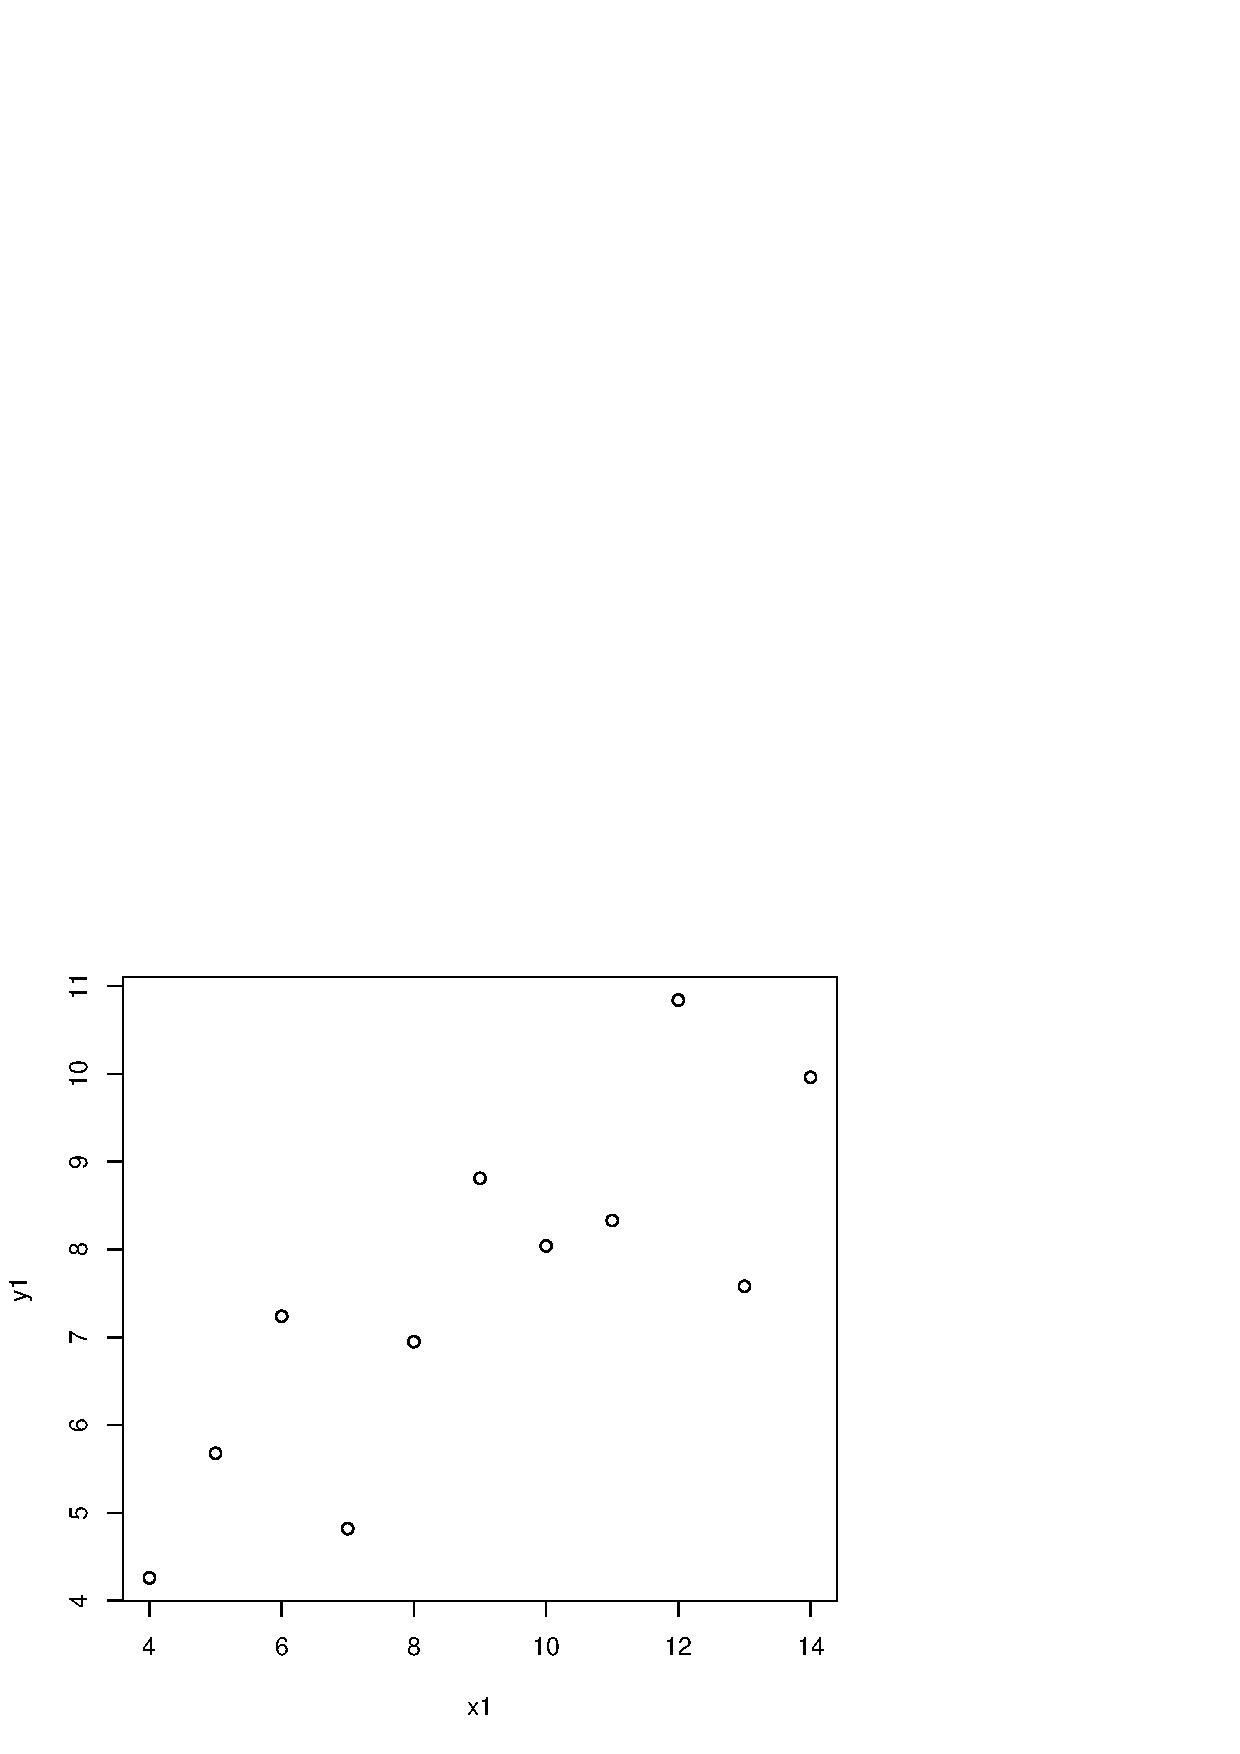
\includegraphics{regression-002}
  \caption{Relation entre \code{y1} et \code{x1} des donn�es
    \texttt{anscombe}}
  \label{fig:relation}
\end{figure}

Le graphique nous montre qu'il est raisonnable de postuler une
relation lin�aire entre les �l�ments de \code{y1} et \code{x1}. On
pose donc le mod�le
\begin{displaymath}
  y_i = \beta_0 + \beta_1 x_i + \varepsilon_i,
\end{displaymath}
o� $y_i$ et $x_i$, $i = 1, \dots, 11$ sont les �l�ments des vecteurs
\code{y1} et \code{x1}, respectivement, et $\varepsilon_i$ est le
terme d'erreur.

C'est avec la fonction \Fonction{lm} (pour \emph{linear model}) que
l'on calcule les estimateurs des coefficients de la r�gression
$\beta_0$ et $\beta_1$. De fa�on simplifi�e, cette fonction prend en
arguments une formule et un \emph{data frame} dans lequel se trouvent
les donn�es relatives aux termes de celle-ci. La fonction \code{lm}
retourne un objet de classe \classe{lm} pour laquelle il existe de
nombreuses m�thodes.
\begin{Schunk}
\begin{Sinput}
> (fit <- lm(y1 ~ x1, data = anscombe))
\end{Sinput}
\begin{Soutput}
Call:
lm(formula = y1 ~ x1, data = anscombe)

Coefficients:
(Intercept)           x1  
     3.0001       0.5001  
\end{Soutput}
\begin{Sinput}
> class(fit)
\end{Sinput}
\begin{Soutput}
[1] "lm"
\end{Soutput}
\end{Schunk}


\section{Analyse des r�sultats}
\label{regression:analyse}

Le r�sultat de la fonction \fonction{lm} est une liste dont on peut
extraire manuellement les diff�rents �l�ments (consulter la rubrique
d'aide). Gr�ce � quelques fonctions g�n�riques disposant d'une m�thode
pour les objets de classe \classe{lm}, il est toutefois facile et
intuitif d'extraire les principaux r�sultats d'une r�gression:
\begin{enumerate}
\item \fonction{coef} ou \fonction{coefficients} extraient les
  coefficients $\hat{\beta}_0$ et $\hat{\beta}_1$ de la r�gression;
\item \fonction{fitted} extrait les valeurs ajust�es $\hat{y}_i =
  \hat{\beta}_0 + \hat{\beta}_1 x_i$;
\item \fonction{residuals} extrait les r�sidus $y_i - \hat{y}_i$;
\item \fonction{deviance} retourne la somme des carr�s des r�sidus
  $\mathrm{SSR} = \sum_{i=1}^n (y_i - \hat{y}_i)^2$;
\item \fonction{df.residual} \R extrait le nombre de degr�s de libert�
  de la somme des carr�s des r�sidus (\textsf{R} seulement).
\end{enumerate}

La fonction g�n�rique \fonction{summary} pr�sente les informations
ci-dessus de mani�re facile � consulter. Plus pr�cis�ment, le sommaire
de la r�gression contient, outre le mod�le utilis� et les estimateurs
des coefficients de la r�gression: les r�sultats des tests $t$, la
valeur du coefficient de d�termination
\begin{displaymath}
  R^2 = 1 - \frac{\sum_{i=1}^n (y_i - \hat{y}_i)^2}{\sum_{i=1}^n
    (y_i - \bar{y})^2}
\end{displaymath}
et, dans \textsf{R} \R seulement, du coefficient de d�termination
ajust�
\begin{displaymath}
  R_a^2 = 1 - (1 - R^2) \frac{n - 1}{n - p - 1},
\end{displaymath}
ainsi que le r�sultat du test $F$ global.

La fonction \Fonction{confint} \R calcule les intervalles de confiance
des param�tres de la r�gression (\textsf{R} seulement).

D'autre part, le tableau d'analyse de variance (s�quentiel, en
r�gression multiple) est calcul� avec la fonction g�n�rique
\fonction{anova}.

Pour ajouter la droite de r�gression au graphique cr�� au d�but de
l'analyse, utiliser la fonction \fonction{abline}, qui dispose elle
aussi d'une m�thode pour les objets de classe \code{lm}.


\section{Diagnostics}
\index{regression@r�gression!diagnostics}
\label{regression:diagnostics}

Les statistiques servant � mesurer la qualit� d'un mod�le de
r�gression ($R^2$, $R^2$ ajust�, statistiques $t$ et $F$) sont
calcul�es par les fonctions \fonction{summary} et \fonction{anova}.

La m�thode de la fonction \fonction{plot} pour les objets de classe
\classe{lm} produit une s�rie de six graphiques (quatre dans
\textsf{R} avant la version 2.2.0) permettant de juger de la qualit�
d'une r�gression.  Consulter la rubrique d'aide de la fonction
\fonction{plot.lm} pour plus de d�tails.


\section{Mise � jour des r�sultats et pr�vision}
\index{regression@r�gression!pr�vision}
\label{regression:prevision}

Il peut arriver que, une fois la mod�lisation d'un ensemble de donn�es
effectu�e, il soit n�cessaire d'ajouter ou de modifier une ou
plusieurs donn�es ou variables. Plut�t que de reprendre toute la
mod�lisation avec la fonction \code{lm}, il peut alors s'av�rer plus
simple et �l�gant d'utiliser la fonction \fonction{update}.
\begin{Schunk}
\begin{Sinput}
> update(fit, ~. + x4)
\end{Sinput}
\begin{Soutput}
Call:
lm(formula = y1 ~ x1 + x4, data = anscombe)

Coefficients:
(Intercept)           x1           x4  
    4.33291      0.45073     -0.09873  
\end{Soutput}
\end{Schunk}

Le calcul de pr�visions et d'intervalles de confiance et de pr�vision
se fait avec la fonction g�n�rique \fonction{predict} et sa m�thode
pour les objets de classe \code{lm}. Par d�faut, \fonction{predict}
calculera les pr�visions pour les valeurs $x_i$, $i = 1, \dots, n$.
Par cons�quent, le r�sultat de \fonction{predict} sera le m�me que
celui de \fonction{fitted}:
\begin{Schunk}
\begin{Sinput}
> all.equal(predict(fit), fitted(fit))
\end{Sinput}
\begin{Soutput}
[1] TRUE
\end{Soutput}
\end{Schunk}
Comme on souhaite g�n�ralement pr�voir la r�ponse pour d'autres
valeurs de la variable ind�pendante, on sp�cifiera celles-ci par le
biais d'un \emph{data frame} pass� � \fonction{predict} avec l'option
\argument{newdata}.

Le calcul des intervalles de confiance et de pr�vision diff�re entre
S-Plus et \textsf{R}. Dans \Splus S-Plus, les intervalles de confiance
en chaque point seront calcul�s par \fonction{predict} avec l'option
\code{ci.fit = T}\indexargument{ci.fit}, alors que les intervalles de
pr�vision le sont avec \texttt{pi.fit = T}\indexargument{pi.fit}. Il
est par cons�quent possible de calculer en un seul appel �
\fonction{predict} les deux types d'intervalles. Le niveau de
confiance est sp�cifi� avec l'option \argument{conf.level} ($0,95$ par
d�faut).

Si un ou plusieurs intervalles de confiance sont calcul�s, le r�sultat
de \fonction{predict} est une liste nomm�e dont les �l�ments sont
\verb=$fit=, \verb=$ci.fit= et \verb=$pi.fit= (et ce peu importe le
nom de l'objet contenant le mod�le lin�aire).

Dans \R \textsf{R}, il n'est pas possible de calculer les deux types
d'intervalles en un seul appel � \fonction{predict}. Pour calculer les
intervalles de confiance, on utilisera l'option
\verb!interval="confidence"!\indexargument{interval}, alors que pour
les intervalles de pr�vision on utilise \verb!interval="prediction"!.
Le niveau de confiance est d�termin� avec l'option \argument{level}. Le
r�sultat est une matrice de trois colonnes dont la premi�re contient
les pr�visions et les deux autres les bornes inf�rieures
(\code{lwr}) et sup�rieures (\code{upr}) des intervalles de
confiance.

Les limites des intervalles de confiance peuvent �tre ajout�es au
graphique des donn�es avec les fonctions \fonction{matlines} ou
\fonction{matplot} \R (\textsf{R} seulement). Consulter les rubriques
d'aide et les exemples pour de plus amples d�tails.

\index{regression@r�gression|)}


\section{Exemples}
\label{regression:exemples}

\lstinputlisting{regression.R}


\section{Exercices}
\label{regression:exercices}

\begin{exercice}
  Importer dans S-Plus ou \textsf{R} l'ensemble de donn�es
  \texttt{steam.dat} se trouvant dans le site Internet
  \begin{quote}
    \url{http://vgoulet.act.ulaval.ca/pub/data/}
  \end{quote}
  � l'aide de la fonction \fonction{read.table}. Les trois premi�re
  lignes du fichier sont des lignes de commentaires d�butant par le
  caract�re \code{\#}. La quatri�me ligne contient les �tiquettes
  des colonnes.
\end{exercice}

\begin{exercice}
  Rendre les colonnes individuelles de l'ensemble de donn�es
  \texttt{steam} visibles dans l'espace de travail.
\end{exercice}

\begin{exercice}
  Faire (m�me � l'aveuglette) l'analyse de r�gression de la variable
  \code{Y} en fonction de la variable \code{X7} des donn�es
  \texttt{steam}.
  \begin{enumerate}
  \item �valuer visuellement le type de relation pouvant exister entre
    \code{Y} et \code{X7}.
  \item �valuer les coefficients d'une r�gression lin�aire entre
    \code{Y} et \code{X7} et ajouter la droite de r�gression ainsi
    obtenue au graphique cr�� en (a).
  \item R�p�ter la partie (b) en for�ant la droite de r�gression �
    passer par l'origine $(0, 0)$. Quel mod�le semble le plus
    appropri�?
  \item Le coefficient de d�termination $R^2$ mesure la qualit� de
    l'ajustement d'une droite de r�gression aux donn�es. Calculer le
    $R^2$ pour les mod�les en (b) et (c).  Obtient-on les m�mes
    r�sultats que ceux donn�s par \fonction{summary}? Semble-t-il y
    avoir une anomalie?
  \item Calculer les pr�visions de chaque mod�le pour quelques valeurs
    choisies de la variable ind�pendante.
  \item Calculer les intervalles de confiance et de pr�vision pour
    tous les points de \code{X7} (bref, ne pas utiliser
    \texttt{newdata}). Ajouter les limites inf�rieures et sup�rieures
    des intervalles au graphique cr�� pr�c�demment. Utiliser des types
    de lignes (option \code{lty}) et des couleurs (option
    \code{col}) diff�rents pour chaque ensemble de limites.
  \end{enumerate}
\end{exercice}

\begin{exercice}
  R�p�ter l'exercice pr�c�dent en ajoutant la variable \code{X5}
  � l'analyse, transformant ainsi le mod�le de r�gression lin�aire
  simple en un mod�le de r�gression multiple.
\end{exercice}

%%% Local Variables:
%%% mode: latex
%%% TeX-master: "introduction_programmation_S"
%%% End:

\include{ts}

\appendix
\chapter{GNU Emacs et ESS: la base}
\index{Emacs|(}
\label{ess}

Emacs est l'�diteur de texte des �diteurs de texte. Bien que
d'abord et avant tout un �diteur pour programmeurs (avec des modes
sp�ciaux pour une multitude de langages diff�rents), c'est �galement
un environnement id�al pour travailler sur des documents \LaTeX,
interagir avec \textsf{R}, S-Plus, SAS ou SQL, ou m�me pour lire son
courrier �lectronique.

L'auteur du pr�sent ouvrage donne acc�s � une version simple �
installer et augment�e de quelques ajouts de la plus r�cente version
de GNU Emacs pour Windows.  Consulter le site Internet
\begin{quote}
  \url{http://vgoulet.act.ulaval.ca/emacs/}
\end{quote}

Cette annexe passe en revue les quelques commandes essentielles �
con\-na�tre pour commencer � travailler avec GNU Emacs et le mode ESS.
L'ouvrage de \cite{LearningEmacs} constitue une excellente r�f�rence
pour l'apprentissage plus pouss� de l'�diteur.


\section{Mise en contexte}

Emacs est le logiciel �tendard du projet GNU (�\emph{GNU is not
  Unix}�), dont le principal commanditaire est la \emph{Free Software
  Foundation}.

\begin{itemize}
\item Distribu� sous la GNU \emph{General Public License} (GPL),
  donc gratuit, ou �libre�.
\item Le nom provient de �\emph{Editing MACroS}�.
\item La premi�re version de Emacs a �t� �crite par Richard M.\ 
  Stallman, pr�sident de la FSF.
\end{itemize}

\section{Configuration de l'�diteur}
\index{Emacs!configuration}

Une des grandes forces de Emacs est d'�tre configurable � l'envi.

\begin{itemize}
\item Depuis la version 21, le menu \texttt{Customize} rend la
  configuration ais�e.
\item Une grande part de la configuration provient du fichier
  \texttt{.emacs}:
  \begin{itemize}
  \item nomm� \texttt{.emacs} sous Linux et Unix, Windows 2000 et
    Windows XP;
  \item sous Windows 95/98/Me, utiliser plut�t \texttt{\_emacs}.
  \end{itemize}
\end{itemize}


\section{\emph{Emacs-ismes} et \emph{Unix-ismes}}

\begin{itemize}
\item Un \emph{buffer} contient un fichier ouvert (�\emph{visited}�).
  �quivalent � une fen�tre dans Windows.
\item Le \emph{minibuffer} est la r�gion au bas de l'�cran Emacs o�
  l'on entre des commandes et re�oit de l'information de Emacs.
\item La ligne de mode (�\emph{mode line}�) est le s�parateur
  horizontal contenant diverses informations sur le fichier ouvert et
  l'�tat de Emacs.
\item Toutes les fonctionnalit�s de Emacs correspondent � une commande
  pouvant �tre tap�e dans le \emph{minibuffer}.  \texttt{M-x} d�marre
  l'invite de commande.
\item Dans les d�finitions de raccourcis claviers:
  \begin{itemize}
  \item \texttt{C} est la touche \texttt{Ctrl} (\texttt{Control});
  \item \texttt{M} est la touche \texttt{Meta}, qui correspond � la
    touche \texttt{Alt} de gauche sur un PC;
  \item \texttt{ESC} est la touche \texttt{�chap} (\texttt{Esc}) et
    est �quivalente � \texttt{Meta};
  \item \texttt{SPC} est la barre d'espacement;
  \item \texttt{RET} est la touche Entr�e.
  \end{itemize}
\item Le caract�re \verb=~= repr�sente le dossier vers lequel pointe
  la variable d'environnement \texttt{\$HOME} (Unix) ou
  \texttt{\%HOME\%} (Windows).
\item La barre oblique (\texttt{/}) est utilis�e pour s�parer les
  dossiers dans les chemins d'acc�s aux fichiers, m�me sous Windows.
\item En g�n�ral, il est possible d'appuyer sur \texttt{TAB} dans le
  \emph{minibuffer} pour compl�ter les noms de fichiers ou de
  commandes.
\end{itemize}


\section{Commandes d'�dition de base}

Il n'est pas vain de lire le tutoriel de Emacs, que l'on d�marre avec
\begin{quote}
  \texttt{C-h t}
\end{quote}
  
Pour une liste plus exhaustive des commandes Emacs les plus
importantes, consulter la \emph{GNU Emacs Reference Card}, dans le
fichier
\begin{quote}
  \url{.../emacs-21.x/etc/refcard.ps}
\end{quote}

\enlargethispage{5mm}
\begin{itemize}
\item Pour cr�er un nouveau fichier, ouvrir un fichier n'existant
  pas.\index{Emacs!nouveau fichier}
\item Principales commandes d'�dition avec, entre parenth�ses, le nom
  de la commande correspondant au raccourci clavier:
  \begin{ttscript}{C-x C-w}
    \raggedright
  \item[\emacs{C-x C-f}] ouvrir un fichier (\texttt{find-file})
  \item[\emacs{C-x C-s}] sauvegarder
    (\texttt{save-buffer})\index{Emacs!sauvegarder}
  \item[\emacs{C-x C-w}] sauvegarder sous
    (\texttt{write-file})\index{Emacs!sauvegarder sous}
  \item[\emacs{C-x k}] fermer un fichier (\texttt{kill-buffer})
  \item[\emacs{C-x C-c}] quitter Emacs
    (\texttt{save-buffers-kill-emacs}) \\[\baselineskip]
  \item[\emacs{C-g}] bouton de panique: quitter!
    (\texttt{keyboard-quit})
  \item[\emacs{C-\_}] annuler (pratiquement illimit�); aussi
    \emacs{C-x u} (\texttt{undo}) \\[\baselineskip]
  \item[\emacs{C-s}] recherche incr�mentale avant
    (\texttt{isearch-forward})
  \item[\emacs{C-r}] Recherche incr�mentale arri�re
    (\texttt{isearch-backward})
  \item[\emacs{M-\%}] rechercher et remplacer
    (\texttt{query-replace})\index{Emacs!rechercher et remplacer}
    \\[\baselineskip]
  \item[\emacs{C-x b}] changer de \emph{buffer}
    (\texttt{switch-buffer})
  \item[\emacs{C-x 2}] s�parer l'�cran en deux fen�tres
    (\texttt{split-window-vertically})
  \item[\emacs{C-x 1}] conserver uniquement la fen�tre courante
    (\texttt{delete-other-windows})
  \item[\emacs{C-x 0}] fermer la fen�tre courante
    (\texttt{delete-window})
  \item[\emacs{C-x o}] aller vers une autre fen�tre lorsqu'il y en a
    plus d'une (\texttt{other-window})
  \end{ttscript}
\end{itemize}


\section{S�lection de texte}
\index{Emacs!s�lection}  
\label{ess:selection}

La s�lection de texte fonctionne diff�remment du standard Windows.

\begin{itemize}
\item Les raccourcis clavier standards sous Emacs sont:
  \begin{ttscript}{C-SPC}
    \raggedright
  \item[\emacs{C-SPC}] d�bute la s�lection (\texttt{set-mark-command})
  \item[\emacs{C-w}] couper la s�lection (\texttt{kill-region})
  \item[\emacs{M-w}] copier la s�lection (\texttt{kill-ring-save})
  \item[\emacs{C-y}] coller (\texttt{yank})
  \item[\emacs{M-y}] remplacer le dernier texte coll� par la
    s�lection pr�c�dente (\texttt{yank-pop})
  \end{ttscript}
\item Il existe quelques extensions de Emacs permettant d'utiliser les
  raccourcis clavier usuels de Windows (\texttt{C-c}, \texttt{C-x},
  \texttt{C-v}); voir
  \url{http://www.emacswiki.org/cgi-bin/wiki/CuaMode}.
\end{itemize}
\index{Emacs|)}

\section{Mode ESS}
\index{ESS|(}

Le mode ESS (\emph{Emacs Speaks Statistics}) permet d'interagir avec
des logiciels statistiques (S-Plus, \textsf{R}, SAS, etc.) depuis
Emacs. Ce mode est install� dans la version modifi�e de GNU Emacs
distribu�e dans le site Internet
\url{http://vgoulet.act.ulaval.ca/emacs/}

\begin{itemize}
\item Voir le fichier
  \begin{quote}
    \texttt{.../emacs-21.x/site-lisp/ess/doc/html/index.html}
  \end{quote}
  pour la documentation compl�te.
\item Deux modes mineurs: \texttt{ESS} pour les fichiers de script
  (code source) et \texttt{iESS} pour l'invite de commande.
\item Une fois install�, le mode mineur \texttt{ESS} s'active
  automatiquement en �ditant des fichiers avec l'extension \texttt{.S}
  ou \texttt{.R}.
\item Pour d�marrer un processus S et activer le mode mineur
  \texttt{iESS}, entrer l'une des commandes \texttt{S}, \texttt{Sqpe}
  ou \texttt{R} dans l'invite de commande de Emacs (voir aussi
  l'annexe \ref{s-plus_windows}). Par exemple, pour d�marrer un
  processus \textsf{R} � l'int�rieur m�me de Emacs, on fera
  \begin{quote}
    \ttfamily M-x R RET
  \end{quote}
\item Commandes les plus fr�quemment employ�es � la ligne de commande
  (mode \texttt{iESS}):
  \begin{ttscript}{C-c C-c}
    \raggedright
  \item[\ess{C-c C-e}] replacer la derni�re ligne au bas de la
    fen�tre (\texttt{comint-show-maximum-output})
  \item[\ess{M-h}] s�lectionner le r�sultat de la derni�re commande
    (\texttt{mark-paragraph})
  \item[\ess{C-c C-o}] effacer le r�sultat de la derni�re commande
    (\texttt{comint-delete-output})
  \item[\ess{C-c C-v}] aide sur une commande S
    (\texttt{ess-display-help-on-object})
  \item[\ess{C-c C-q}] terminer le processus S
    (\texttt{ess-quit})
  \end{ttscript}
\item Commandes les plus fr�quemment employ�es lors de l'�dition d'un
  fichier de script (mode \texttt{ESS}):
  \begin{ttscript}{C-c C-c}
    \raggedright
  \item[\ess{C-c C-n}] �value la ligne sous le curseur dans le
    processus S (\texttt{ess-eval-line-and-step})
  \item[\ess{C-c C-r}] �value la r�gion s�lectionn�e dans le
    processus S (\texttt{ess-eval-region})
  \item[\ess{C-c C-f}] �value le code de la fonction courante dans
    le processus S (\texttt{ess-eval-function})
  \item[\ess{C-c C-l}] �value le code du fichier courant dans le
    processus S (\texttt{ess-load-file})
  \item[\ess{C-c C-v}] aide sur une commande S
    (\texttt{ess-display-help-on-object})
  \item[\ess{C-c C-s}] changer de processus (utile si l'on a plus
    d'un processus S actif)
  \end{ttscript}
\item Raccourcis clavier utiles lors de la consultation des rubriques
  d'aide:
  \begin{ttscript}{m, m}
    \raggedright
  \item[h] ouvrir une nouvelle rubrique d'aide, par d�faut pour le mot
    se trouvant sous le curseur (\texttt{ess-display-help-on-object})
  \item[n, p] aller � la section suivante (\texttt{n}) ou pr�c�dente
    (\texttt{p}) de la rubrique (\texttt{ess-skip-to-next-section},
    \texttt{ess-skip-to-previous-section})
  \item[l] �valuer la ligne sous le curseur; pratique pour ex�cuter
    les exemples (\texttt{ess-eval-line-and-step})
  \item[r] �valuer la r�gion s�lectionn�e (\texttt{ess-eval-region})
  \item[q] retourner au processus ESS en laissant la rubrique d'aide
    visible (\texttt{ess-switch-to-end-of-ESS})
  \item[x] fermer la rubrique d'aide et retourner au processus ESS
    (\texttt{ess-kill-buffer-and-go})
  \end{ttscript}
\end{itemize}
\index{ESS|)}


\section{Session de travail type}
\label{ess:session_travail}

On d�crit, dans cette section, les diff�rentes �tapes et principaux
raccourcis claviers d'une session de travail type avec S-Plus ou
\textsf{R}, Emacs et ESS.

\begin{enumerate}
\item D�terminer le dossier de travail et le cr�er au besoin.
  Normalement, le dossier de travail pour S-Plus ou \textsf{R} sera le
  m�me que celui o� les fichiers de script sont sauvegard�s. Si l'on
  pr�voit sauvegarder des objets S, il est important de choisir un
  nouveau dossier pour le projet.
\item Lancer Emacs et d�marrer un processus S dans le dossier de
  travail d�termin� ci-dessus.
  \begin{itemize}
  \item \code{M-x R RET} ou \code{M-x Sqpe RET}
  \end{itemize}
\item Ouvrir un fichier de script dans lequel on sauvegardera le code
  source.
  \begin{itemize}
  \item \emacs{C-x C-f} pour ouvrir un fichier existant ou un nouveau
    fichier.
  \end{itemize}
\item Composer le code. Lors de cette �tape, on se d�placera souvent
  du fichier de script � la ligne de commande afin d'essayer diverses
  expressions. On ex�cutera �galement des parties seulement du code se
  trouvant dans le fichier de script.
  \begin{itemize}
  \item \emacs{C-x o} pour se d�placer de la fen�tre de script � la
    ligne de commande et vice-versa.
  \item \ess{C-c C-e} pour replacer le curseur � la ligne de commande
    et au bas de la fen�tre.
  \item \ess{C-c C-o} pour effacer le r�sultat de la derni�re
    commande, surtout s'il est tr�s long.
  \item \ess{C-c C-n} pour ex�cuter une ligne du fichier de script.
  \item \ess{C-c C-r} pour ex�cuter une r�gion du fichier de script
    (voir la section \ref{ess:selection} pour s�lectionner une r�gion).
  \item \ess{C-c C-f} pour d�finir une fonction.
  \end{itemize}
\item Sauvegarder le fichier de script. Les quatri�me et cinqui�me
  caract�res de la ligne de mode changent de \verb|**| � \verb|--|.
  \begin{itemize}
  \item \emacs{C-x C-s} pour sauvegarder le fichier de script.
  \end{itemize}
\item Il est �galement possible de sauvegarder le texte de la session
  interactive (la ligne de commande). Il est recommand� de nommer de
  telles transcriptions de la session de travail avec une extension
  \texttt{.St} ou \texttt{.Rt}. En effet, ESS poss�de un mode sp�cial
  pour les transcriptions. Consulter � cet effet le chapitre 5 de la
  documentation de ESS.
  \begin{itemize}
  \item \emacs{C-x C-s} pour sauvegarder le texte de la session.
  \end{itemize}
\item Quitter le processus S. Utiliser la commande ESS pour ce faire
  puisque ESS se chargera de fermer tous les fichiers associ�s au
  processus S. � moins qu'il ne contienne des objets importants,
  l'espace de travail \R en \textsf{R} n'est habituellement pas
  sauvegard�.
  \begin{itemize}
  \item \ess{C-c C-q} pour quitter le processus S.
  \end{itemize}
\end{enumerate}


%%% Local Variables: 
%%% mode: latex
%%% TeX-master: "introduction_programmation_S"
%%% End: 

\chapter{Utilisation de ESS et S-Plus sous Windows}
\index{Emacs!et S-Plus|(}
\label{s-plus_windows}

L'utilisation de \textsf{R} et S-Plus avec ESS dans Emacs est
virtuellement identique sous Unix. Sous Windows, la proc�dure est
exactement la m�me que sous Unix pour \textsf{R}, mais l'interface
avec S-Plus est l�g�rement plus compliqu�e.

Avant toute chose, il faut s'assurer d'avoir une installation de
Emacs, ESS et S-Plus fonctionnelle. L'installation de la version
modifi�e de Emacs distribu�es dans le site Internet
\begin{quote}
  \url{http://vgoulet.act.ulaval.ca/pub/emacs/}
\end{quote}
devrait permettre de satisfaire cette exigence rapidement.

Il y a deux fa�ons de travailler avec S-Plus depuis Emacs sous
Windows: tout dans Emacs ou une combinaison de Emacs et de l'interface
graphique de S-Plus.


\section{Tout dans Emacs}

Cette approche est similaire � celle favoris�e sous Unix ainsi qu'avec
\textsf{R}. Un processus S-Plus est d�marr� � l'int�rieur m�me de
Emacs, un fichier de script (habituellement avec une extension
\texttt{.S}) est ouvert dans Emacs et les lignes de ce fichier sont
ex�cut�es dans le processus S-Plus. La fen�tre Emacs est alors scind�e
en deux. C'est l'approche pr�n�e � la section
\ref{presentation:strategies}.

Le truc consiste ici � utiliser non pas l'ex�cutable
\texttt{splus.exe} (qui est l'interface graphique), mais plut�t
l'interface en ligne de commande, plus simple et rapide. L'ex�cutable
est \texttt{sqpe.exe}. Pour d�marrer une session S-Plus dans Emacs, on
fera donc

\begin{quote}
  \ttfamily M-x Sqpe RET
\end{quote}
Lorsque demand�, on sp�cifie le dossier de travail. Une fois l'invite
de commande S-Plus obtenue, on pourra ex�cuter des lignes du fichier
de script dans le processus S-Plus avec \texttt{C-c C-n}, \texttt{C-c
  C-f}, etc.

Il y a toutefois un os avec cette approche: aucun p�riph�rique
graphique n'est disponible. Sauf depuis la version 6.1 de S-Plus: on
peut utiliser un p�riph�rique graphique Java. Afin de pouvoir
l'utiliser, il faut ex�cuter les deux lignes suivantes \emph{avant} de
cr�er un graphique:
\begin{Schunk}
  \begin{Sinput}
> library(winjava)
> java.graph()
  \end{Sinput}
\end{Schunk}

Il est possible d'automatiser ce processus en sauvegardant ces deux
lignes dans un fichier nomm� \texttt{S.init} dans le dossier de
travail. Le contenu de ce fichier sera ex�cut� � chaque fois que
S-Plus sera d�marr� dans ce dossier.


\section[Combinaison Emacs et S-Plus GUI]{Combinaison Emacs et interface graphique de S-Plus}

Cette option est moins �l�gante que la pr�c�dente, mais certains
pourraient lui voir comme avantage d'utiliser l'interface graphique
(GUI) de S-Plus. En fin de compte, la proc�dure ci-dessous revient �
remplacer par Emacs la fen�tre d'�dition de script incluse dans
S-Plus.

En faisant
\begin{quote}
  \ttfamily M-x S RET
\end{quote}
� l'int�rieur de Emacs, une nouvelle session graphique de S-Plus sera
d�marr�e (il faut �tre patient, les n�gociations entre les deux
logiciels peuvent prendre du temps). On se retrouve donc avec deux
fen�tres: une pour Emacs et une pour S-Plus.

Ouvrir un fichier de script dans Emacs et ex�cuter les lignes de comme
ci-dessus. Les lignes de code seront ex�cut�es dans l'interface
graphique. En d'autres mots, le code source se trouve dans une fen�tre
(Emacs) et les r�sultats de ce code source dans une autre (S-Plus). Il
faut bien disposer les fen�tres c�te � c�te pour que cette strat�gie
se r�v�le minimalement efficace.

L'information ci-dessus se trouve dans la documentation de ESS.

\index{Emacs!et S-Plus|)}

%%% Local Variables: 
%%% mode: latex
%%% TeX-master: "introduction_programmation_S"
%%% End: 

\include{rng}
\include{simulation}
\include{fdl}
\chapter*{Réponses des exercices}
\label{reponses}
\addcontentsline{toc}{chapter}{Réponses des exercices}
\markboth{Réponses des exercices}{Réponses des exercices}

\input{solutions-bases}
\input{solutions-operateurs}
\input{solutions-exemples}
\input{solutions-fonctions}
\input{solutions-avance}
\input{solutions-optimisation}
\input{solutions-rng}

%%% Local Variables:
%%% mode: latex
%%% TeX-engine: xetex
%%% TeX-master: "introduction_programation_r"
%%% coding: utf-8
%%% End:


\bibliographystyle{agsm}
\bibliography{stat,informatique}

\cleardoublepage
\printindex

\cleardoublepage
\cleartoverso

\pagestyle{empty}
\vspace*{\fill}\hfill
\large\ttfamily ISBN \ISBN

\end{document}

%%% Local Variables: 
%%% mode: latex
%%% TeX-master: t
%%% End: 
